\documentclass[11pt,a4paper]{article}

%
% Dependencies
%

\usepackage[utf8]{inputenc}
\usepackage[T1]{fontenc}
\usepackage[ngerman]{babel}
\usepackage{lmodern}
\usepackage{ragged2e}
\usepackage{amsmath}
\usepackage{graphicx}
\usepackage{rotating}
\usepackage[export]{adjustbox}
\usepackage{placeins}
\usepackage{csquotes}
\usepackage[hidelinks]{hyperref}
\usepackage{ltablex}
\usepackage{booktabs}
\usepackage{caption}
\usepackage{fmtcount}
\usepackage{fancyhdr}
\usepackage{multirow}
\usepackage{afterpage}

\usepackage[
    backend = biber,
    style = alphabetic,
    citestyle = alphabetic,
    autocite = superscript,
]{biblatex}


%
% Configuration
%

% took the following from: https://bastian.rieck.ru/blog/posts/2016/biblatex_superscript_citations/
\DeclareCiteCommand{\supercite}[\mkbibsuperscript]{}{[\usebibmacro{citeindex}\usebibmacro{cite}\usebibmacro{postnote}]}{\supercitedelim}{}


\pagestyle{fancy}
\renewcommand{\headrulewidth}{0pt}
\fancyhf{}

% page number at foot center, suppress it for float pages
\fancyfoot[C]{\iffloatpage{}{\thepage}}

%\newcommand{\paragraphheader}[1]{\paragraph{#1}\mbox{}\\}
%\newcommand{\paragraphheader}[1]{\paragraph{#1}\mbox{}}
%\newcommand{\paragraphheader}[1]{\paragraph{#1}}


%
% Custom Commands
%

\newcommand{\highlight}[1]{\textit{\textbf{#1}}}

\newcommand{\refimg}[1]{\textit{\nameref{#1}}}
\newcommand{\refgoal}[1]{\textit{\nameref{#1}}}
\newcommand{\refsec}[1]{\textit{\nameref{#1}}}


\newcommand{\source}[1]{\caption*{\textit{(Quelle: {#1})}}}
\newcommand{\ownsource}{\source{eigens erstellt}}

% This command is an alias for newline and is used to break
% pages and "help tex".
% It is an alias so places where they are used are easier to find.
\newcommand{\helptex}{\newline}


%
% Bib Source
%

\addbibresource{projektarbeit.bib}

\begin{document}

    \begin{titlepage} % Suppresses displaying the page number on the title page and the subsequent page counts as page 1

    %\raggedright % Right align the title page

    \rule{1pt}{\textheight} % Vertical line
    \hspace{0.05\textwidth} % Whitespace between the vertical line and title page text
    \parbox[b]{0.97\textwidth}{ % Paragraph box for holding the title page text, adjust the width to move the title page left or right on the page
        \RaggedRight % Right align the title page

        {\fontsize{23pt}{23pt}\selectfont\textbf{Entwicklung einer verteilten agentenbasierten Simulationsplattform mithilfe des Java\-Script Ökosystems, am Beispiel einer Verkehrssimulation.}
        \par}
        \bigskip
        {\large\textit{Projektarbeit im Studiengang Software- und \\ Systemtechnik V. Softwaretechnik (BPO 2015)}\par} % Subtitle or further description
        \bigskip
        {\Large\textsc{Florian Völker 7102143}\par} % Author name, lower case for consistent small caps

        \vspace{0.25\textheight} % Whitespace between the title block and the publisher

        {\noindent Fachhochschule Dortmund} % Publisher and logo
        \bigskip
    }


    \afterpage{
        \null
        \thispagestyle{empty}
        \newpage
    }

\end{titlepage}



    \tableofcontents
    \newpage

    \setlength{\parindent}{0em}
    \setlength{\parskip}{1em}


    \section{Einleitung}


    \subsection{Motivation}

Agentenbasierte Systeme sind in der heutigen Forschung und Softwareentwicklung allgegenwärtig.
Diese Art der Modellierung findet sowohl in der Wirtschaft\autocite{Levy2009} und der Erforschung von sozialem Verhalten\autocite{fang2016} als auch schon in der frühen Verkehrsplanung\autocite{wiedermann1974} Anwendung.

Agentenbasierte Modellierung besticht dabei vor allem durch ihre realitätsnahe Konzipierung.
Ähnlich zu objektorientierter Programmierung werden hier reale Entitäten als Softwarekomponenten spezifiziert.
Dabei stehen bei der agentenbasierten Modellierung der Akteur als \textbf{Agent} und sein Handeln in einem \textbf{System} im Vordergrund.
Die agentenbasierte Modellierung beschreibt allerdings nur das Konzept dieser beiden Komponenten.

Im Kontext der Wirtschaftssimulation ist das Wirtschaftssystem das \textbf{System} und die \textbf{Akteure} beispielweise Käufer, Verkäufer oder Produ-\linebreak zenten\autocite{agenteco2015}.
Im Falle einer Verkehrssimulation wäre dies das Verkehrssystem mit Autofahrern, Fußgängern und Radfahrern\autocite{fujii2017}.

In beiden Fällen hängen die implementierten Akteure stark von dem Ziel der Simulation ab.
Sollte man beispielweise Micro-Verhalten eines Verkehrssystems simulieren wollen, um zu ermitteln, welche Gründe es für Stau gibt, könnte es vorteilhaft sein, den Autofahrer nicht zu verallgemeinern, sondern spezielle Ausprägungen seines Verhaltens wie beispielweise Sonntags-Fahrer, Pendler oder Raser zu implementieren.

Der Agent ist dabei ein Typ von Akteuren, die durch ihr Verhalten im System zusammengefasst werden könne.
Er definiert primär das Verhalten in Form der Auswahl einer Aktion im System auf Grundlage der wahrgenommenen Umgebung und seines inneren Zustands.
Das System definiert hingegen die Realität und spezifiziert damit, welche möglichen Aktionen ein Agent und welches Resultat eine Handlung hat, und definiert gleichzeitig damit implizit die Relation von Agenten\autocite{salamon2011}.

Besonders wichtig dabei ist, dass ein Agent nur auf Grundlage von lokalem, beschränktem Wissen agiert.
Sein Verhalten ist oft sehr einfach gehalten und definiert häufig einen diskreten Übergang von einem zu einem anderen Zustand.\autocite{salamon2011}

Der große Vorteil dieser Art der Modellierung besteht darin, dass diese einfachen Regeln dann durch ihre Wechselwirkungen ein komplexes, sogenanntes \textbf{emergentes Verhalten} erzeugen.

Dieses emergente Verhalten ist dann auch oft der Untersuchungsgegenstand, wobei es dann das Ziel sein kann, es zu erkennen, zu erzeugen oder zu vermeiden.\autocite{chen2007}
So könnte bei einem Verkehrssystem versucht werden das emergente Verhalten \textit{Stau} zu vermeiden oder zu verringern.

Da dieses Verhalten jedoch nicht explizit definiert ist, gelingt dies nur, indem das System angepasst (Menge der Spuren, Geschwindigkeitsbegrenzungen etc.) oder das Verhalten der Agenten modifiziert wird (Abstandseinhaltung, Beschleunigung etc.).

Jedoch ist der Prozess, von einer Ausgangsdefinition zu einer Definition für das System bzw.\ dessen Agenten zu gelangen, die das gewünschte Verhalten zeigen, nicht trivial und lässt sich im Regelfall nur iterativ approximie-\linebreak ren.\autocite{nikolic2011}

Bei dieser iterativen Konzipierung und Entwicklung kann eine entsprechend darauf ausgerichtete Plattform stark unterstützen.

Viele solcher Plattformen wurden mithilfe von C/C++ oder Java ent-\linebreak wickelt\autocite{abar2017}, was zum einen erfordert, dass diese Plattformen und ihre Abhängigkeiten installiert werden müssen, und zum anderen, dass die Agenten mit dieser oder einer kompatiblen Sprache erstellt werden.

Dies resultiert in einer Einstiegshürde, die sich durch die Verwendung eines Webbrowsers und damit der Sprache JavaScript für die Programmierung verringern ließe.

Deshalb soll durch diese Arbeit überprüft werden, ob mit den Technologien des JavaScript Ökosystems eine solche Simulationsplattform geschaffen werden kann, die erweiterbar ist und sich zur performanten Darstellung des Simulationszustandes eignet.

Dies soll anhand einer exemplarisch abstrakten Verkehrssimulation geschehen.

%\begin{itemize}
%\item Interaktionen von lokal agierenden Verkehrsteilnehmern führen zu emergentem Verhalten welches für den einzelnen Autofahrer schwer zu greifen ist.
%\item Wechselwirkungen können zu Kaskaden und damit zum Zusammenbruch des Verkehrsflusses führen, die eigentlichen Ursachen sind allerdings meist schwer nachzuvollziehen.
%\item Diese Phänomäne sind für mich sehr spannend, insofern sie dem Verkehr eine Eigendynamik geben, welche nicht direkt durch einzelne Teilnehmer gesteuert werden.
%\item Mit Simulationssoftware lassen sich solche Phänomäne leichter veranschaulichen und die Ursachen bzw. die Auswirkungen besser nachvollziehen.
%\end{itemize}

%Als Softwareentwickler interessierte ich mich schon immer für komplexe Systeme, Vor allem solche welche viele Beteiligten haben.
%
%Gerade Systeme welche dezentral wirken und keiner übergeordnete Kontrolle unterliegen waren dabei spannend.
%Solche Systeme funktionieren zumeist weil die beteiligten Akteure lokal aber nicht unabhängig voneinander agieren.
%
%Ein Beispiel sind hier Ameisen.
%Sie haben keine Anführer oder Befehlsstrukturen und trotzdem arbeiten tausende von Akteuren zielgerichtet und gemeinschaftlich auf ein Ziel hin.
%
%Dies ist dadurch möglich das alle Akteure auf andere Akteure, Umgebungseigenschaften und Signale achten.
%Da Akteure, in diesem Kontext Ameisen, auf andere Akteure achten, und ihr Verhalten an diese anpassen, entstehen Wechselwirkungen.
%
%Diese Wechselwirkungen lassen die gesamte Ameisenkolonie als eine intelligente Einheit erscheinen.
%Dieses Phänomen nennt man auch emergentes Verhalten.
%Emergent nennt man das System dann, wenn das Verhalten der Akteure auf \textit{lokalen impulsen} basiert, wenn  \textit{nahe andere Akteure} ihr Verhalten beeinflussen, sie untereinander gleichberechtigt sind bzw. es keine Hierarchie gibt und ihr Verhalten mit Regeln modelliert werden kann.
%
%Emergente Systeme haben mich schon immer fasziniert, weil ihr Verhalten intelligent erscheint aber nicht zentral kontrolliert wird.
%Dadurch ist ihre Definition verhältnismäßig einfach, insofern nur die einfachen lokalen Verhaltensweisen der Akteure bestimmt werden müssen, jedoch ist die Abschätzung, welchen Zustand das System nach einer bestimmten Zeit hat, nahezu unmöglich.
%
%Auch in unserer Gesellschaft wirken solche emergenten Systeme.
%Ein klassischen ist die Wirtschaft, welche durch lokal agierende, mit relativ einfachen Regeln definierte Akteure beschrieben werden kann.
%Deren Aktionen im System wirken sich auf andere Akteure aus und erzeugen dadurch kaskadierende Wechselwirkungen.
%
%Conway's Game of Life ist ein anderes, etwas einfacheres System.
%Auch wenn die Regeln des Systems auf weniger als eine DIN A4 Seite passen, ist es fast unmöglich den Endzustand des Systems zu bestimmen.
%
%Ein anderes System, welches Menschen erzeugt haben und welches emergentes Verhalten zeigt ist der Straßenverkehr.
%Auch hier erzeugen lokale Akteure, welche relativ einfache Regeln befolgen, ohne eine übergeordnete Kontrollstruktur zu haben, ein komplexes System, bei dem es so wirkt als hätte es ein gesamtheitliches Verhalten.
%
%Diese Agenten beeinflussen sich gegenseitig, so kann man beispielweise auf seiner aktuellen Spur nur so weit fahren wie es das Auto vor einem erlaubt.
%Auch bei diesem System ist es nahezu unmöglich abzuschätzen welchen Zustand das System nach einer gewissen Zeitspanne hat.
%
%Deshalb möchte ich in dieser Arbeit eine Simulationsplattform schaffen welche es dem Nutzer erlaubt, durch definition dieser einfachen Regeln, abzuschätzen inwieweit selbst kleine Änderungen das Gesamtverhalten des System gravierend verändern kann und dadurch das komplexe Verhalten erfahrbarer zu machen.
%
%\iffalse
%Der Straßenverkehr ist ein äußerst spannendes System.
%Er wird durch strenge Regeln welche alle Teilnehmer einhalten müssen abschätzbar, wird jedoch im Detail durch lokal agierende Beteiligte ausgestaltet.
%Letztere sorgen dafür, dass, in Kombination mit den Wechselwirkungen zwischen den Fahrern, der Straßenverkehr zu einem emergenten System wird.
%Dadurch ist der Verkehrsfluss schlecht abzuschätzen und vor allem nur sehr bedingt zu kontrollieren.
%
%Wenn also beispielweise ein abrupter Spurwechsel zu einem abruptem Bremsmanöver führt, welches dann zu einem Stau ohne Staugrund führt und dieses Stauende sich in einer Kurve befindet, in welche ein anderer Fahrer kollidiert und bei dem Auffahrunfall sein Leben verliert, dann ist es nicht offensichtlich, dass der unbedachte Spurwechsel an dem Unfall beteiligt war.
%
%Diese Art von Phänomene interessieren mich bei dem Straßenverkehr sehr, sie demonstrieren sehr anschaulich wie komplex etwas so alltägliches sein kann.
%Sicherlich helfen solche Erkenntnisse nicht bei dem alltäglichen Verwenden weiter, können jedoch durchaus dabei helfen Straßenabschnitte zu planen oder Gesetzmäßigkeiten anzupassen.
%
%Sollte in der Realität man ein Problem mit diesem System vermuten, dann bedarf es langer Untersuchungen, um die Ursache zu finden.
%Nicht selten lassen sie sich gar nicht finden, da die Umstände nicht wieder hergestellt werden können.
%Auch ist selten der Aufwand in einem angebrachten Verhältnis zu dem eigentlichen Problem.
%Oft könnte schon durch eine einfache Anpassung der Ampelschaltung der Verkehrsfluss stark verbessert werden wodurch indirekte Konsequenzen vermieden werden können.
%
%Selbst wenn dann eine Ursache gefunden worden ist, muss dann noch eine Anpassung geplant werden.
%Dessen Folge lässt sich allerdings so gut wie gar nicht bestimmen außer sie wurde an anderer Stelle bereits erprobt, da es sich hier um ein emergentes System handelt.
%Dieses kann, wenn überhaupt, nur stochastisch abgeschätzt werden.
%Das Straßenverkehrssystem lässt aber selbst das nicht zu.
%
%Aus diesem Grund soll eine Software schaffen, welche es möglich machen soll, diese Phänomene modellhaft nachzustellen und dann die Ursache zu ergründen.
%Im Anschluss an die Findung soll es möglich sein eine Lösung iterativ zu erproben, wodurch es einfacher sein soll reale Auswirkungen abzuschätzen und somit effektiver Lösungen anwenden zu können.
%
%\fi


    \subsection{Ziel}

Das Ziel dieser Arbeit soll es sein, zu ermitteln, ob mithilfe des JavaScript Ökosystems eine Anwendung in einer Client Server Architektur erstellt werden kann, die performant mehrere tausend Fahrzeuge, die durch eine agentenbasierte Modellierung kontrolliert werden, vom Server zum Client übertragen und dreidimensional darstellen kann.

Dafür soll eine solche Test-Anwendung entwickelt und im Anschluss ihre Performanz eingeschätzt werden.
Diese Anwendung soll dafür dem Nutzer die Möglichkeit bieten, mithilfe einer einfachen Schnittstelle einen Agenten zu spezifizieren und innerhalb der Plattform betreiben zu lassen.
Zusätzlich soll der Nutzer in der Lage sein, über eine einfache grafische Schnittstelle ein Straßennetz zu definieren, das er mit dem Agenten zusammen zu einer laufenden Instanz kombinieren kann.
Diese soll dann in Echtzeit anschaulich und plastisch dargestellt werden können.


    \subsection{Verwandte Arbeiten}

Das Feld der agentenbasierten Simulation erstreckt sich über die unterschiedlichsten wissenschaftlichen Bereiche, wie beispielweise von der evolutionären Entwicklung von Organismen über Lieferketten-Optimierung bis hin zu Stadtplanungs-Auswirkungen.
Dabei werden unterschiedliche Geltungsbereiche betrachtet.
Auch unterscheidet sich der Anpassungs-, Konfi\-gurations- oder Implementationsaufwand drastisch\autocite{abar2017}.

Für den Bereich der Verkehrssimulationen gibt es verschiedenste Anwendungen, je nachdem, welche Abstraktionshöhe gewünscht ist.
Eine der weitverbreitetsten für die Simulation von autonomen Verkehrsteilnehmern\autocite{jing2020} ist die MATSim Simulationsplattform, die sich vor allem dadurch auszeichnet, dass sie mehrere Agenten synchron und unabhängig voneinander in der gleichen Simulation betreibt.\autocite{axhausen2016}
Sie kann verwendet werden, um Interaktionen im Kontext weniger Fahrer und ihrer Entscheidungen innerhalb einiger Millisekunden zu berechnen, aber auch dafür eingesetzt werden, den gesamten Verkehr in ganz Deutschland zu simulieren\footnote{\url{https://matsim.org/gallery/germany}}.
Beides gelingt mit den gleichen Agenten.

Andere Anwendungen wie MatLab\footnote{\url{https://de.mathworks.com/products/matlab.html}}, AnyLogic\footnote{\url{https://www.anylogic.com/}} oder NetLogo\footnote{\url{https://ccl.northwestern.edu/netlogo/}} sind generischer werden allerdings auch für die Verkehrssimulation eingesetzt\autocite{jing2020}.

Für die professionelle Stadtplanung kommen viele weitere Anwendungen hinzu, die weniger auf die Fahrer bzw. deren Verhalten abzielen, sondern Aspekte wie den Durchsatz, die Unfallquote, die entstehende Lautstärke, die Funkabdeckung etc. untersuchen wollen.

Diese Anwendungen werden allerdings oft mit anderen Ansätzen oder Agen\-ten-Mischkonzepten entwickelt.
So wird beim Fraunhofer VMC ein stochastischer Ansatz verfolgt, um Informationen über die Belastung eines einzelnen Fahrzeuges bei einer gegebenen Route zu bestimmen\autocite{burger2021}.
Dafür können Routen und konkrete Fahrzeugdetails via Parameter angepasst werden.

DLRs SUMO\footnote{\url{https://www.eclipse.org/sumo/}}, Calipers TransModeler\footnote{\url{https://www.caliper.com/TransModeler/}}, TransCad\footnote{\url{https://www.caliper.com/tcovu.htm}}, PTVs Visum\footnote{\url{https://www.ptvgroup.com/en/solutions/products/ptv-visum/}} und die neu erworbene Produktpalette von Bentley\footnote{\url{https://www.bentley.com/en/products/product-line/mobility-simulation-and-analytics}} mit CUBE, Emme und Dynameq sind Anwendungen, die sich auf die Modellierung von Verkehrsflüssen konzentrieren und für die Infrastrukturplanung verwendet werden.

Diese Arbeiten tangieren diese allerdings nur in der Simulationsdomäne, da die hier zu entwickelnde Anwendung nicht primär den Verkehr modellieren soll, sondern erproben soll, ob sich solch eine Anwendung mit den JavaScript Technologien umsetzen lässt.
Somit verfolgen diese Arbeiten sehr unterschiedliche Entwicklungsziele.

In eine ähnliche Richtung geht die Arbeit von Jozef Méry\autocite{mery2020}, der im Gegensatz dazu eine ähnliche Anwendung im JavaScript Ökosystem entwickelte.
Diese ist jedoch nicht verteilt, sondern wird vollständig im Browser betrieben und konzentriert sich auf die Modellierung durch das Konzept von Predator und Prey\footnote{\url{https://en.wikipedia.org/wiki/Lotka\%E2\%80\%93Volterra_equations}}.
Die Arbeiten von Zehe et al.\autocite{zehe2013} demonstrieren im Kontrast dazu welche weiteren Möglichkeiten sich durch eine verteilte JavaScript-Plattform ergeben würden.



    \subsection{Struktur der Arbeit}

Die hier folgende Arbeit soll die aufgebrachte Zielsetzung und deren Umsetzung beschrieben.
Dafür ist sie in drei Arbeitsschritte bzw. deren Kapitel geteilt.

Begonnen wird bei der Definition der Anforderungen.
Dabei wird zwischen den Funktionalen- und nicht Funktionalen-Anforderungen unterschieden.

Im Anschluss folgt die Beschreibung der Umsetzung in Form des angestrebten Konzeptes.
Dieses untergliedert sich zuerst in die Lösungsstrategie, die grundsätzlich beschreiben soll, welche Struktur die übergeordnete Lösung haben soll.

Darauf folgen die querschnittlichen Konzepte, welche sich vor allem auf die eingesetzten Technologien, ihre Auswahlkriterien so wie deren Eigenschaften beziehen.
Die sich daran anschließende Machbarkeitsvalidierung half dabei einschätzen zu können, ob die Plattform überhaupt machbar war.

Die sich dem anschließenden drei Kapitel gehen dann ins Detail und stellen erst aus Sicht der Bausteine, dann aus dem Blick der Laufzeit und schlussendlich im Sinne der Verteilung die Komponenten und deren Interaktionen dar.
Sie sollen durch sukzessive präzisierung dabei helfen nachvollziehen zu können wie die Anwendung strukturiert ist, wie sie intern funktioniert und welche Überlegungen dabei angestellt worden sind.

Schlussendlich soll innerhalb der Konzipierung noch der Beispielagent und sein Verhalten dargestellt werden.
Als Beispiel wird er hier aufgeführt damit durch ihn erschlossen werden kann, wie strukturell auch dieser Bestandteil funktionieren kann, welche Aspekte dabei zu beachten sind aber auch wie einfach dessen Implementation sein kann.

Die Resultatsbetrachtung stellt dann den Abschluss dar und erlaubt eine gute Übersicht über die Anwendung.
In diesem Kapitel werden dann die Anforderungen evaluiert und eingeschätzt welche Leistungsmerkmale die Plattform nun tatsächlich aufweist um damit auch die Beantwortung der initialen Fragestellung bzw. die Zielerfüllung abschätzen zu können.

Der Ausblick soll danach aber auch aufzeigen, welche Aspekte diese Plattform noch nicht bereitstellt und durch welche Erweiterungen sie noch an Funktionalität bzw. Leistung gewinnen könnte.
Das Fazit fasst dann das Arbeitsergebnis noch einmal zusammen und beantwortet die eingehende Frage abschließend.



    \section{Anforderungserhebung}

Die folgenden Anforderungen wurden für die Anwendung definiert.


    \subsection{Funktionale Anforderungen}

Die hier folgenden Anforderungen wurden für die Test-Implementation spezifiziert, um eine Mindestbenutzbarkeit herzustellen.

\textit{FNC – functional requirement – Funktionale Anforderungen}

\subsubsection{FNC\#01 – Definition eines Straßenlayouts} \label{fnc:define_layout}

Der Nutzer soll in der Lage sein, eine Repräsentation eines Straßenlayouts zu modellieren.
Dieses Modell soll verschiedene signifikante Elemente eines Straßensystems wie beispielweise Geraden, Kurven oder (T-)Kreuzungen beinhalten.

Die Modellierung soll sowohl nachvollziehbar und einfach verwendbar für den Nutzer als auch gut verarbeitbar für den Agenten sein.
Um dafür die Grundlage zu schaffen, soll die Modellierung durch ein gleichmäßiges Raster beschränkt sein.
In jeder Zelle des Rasters kann dann ein Element des Straßennetzes, wie beispielweise eine Kurve, platziert werden.

Damit die Modellierung für den Nutzer zusätzlich vereinfacht wird, soll diese über einen 3D-Editor, wie in \refgoal{fnc:configure_layout} beschrieben, erfolgen.

Nach der Erstellung, bei der noch ein Name und eine optionale Beschreibung vergeben werden können, ist dieses dann für die weitere Verwendung im System hinterlegt.

\subsubsection{FNC\#02 – Inspektion eines Straßenlayouts} \label{fnc:inspect_layout}

Das Straßenlayout soll in einer 3D-Darstellung erfolgen.
Der Nutzer soll dabei in der Lage sein, mithilfe der Maus die Position und die Orientierung der Kamera zu verändern.

Die Modellierung der Darstellung soll an die Realität angelehnt sein und wiedererkennbare Merkmale aufweisen.
Damit ist gemeint, dass ein blauer bzw. himmelähnlicher Hintergrund gezeichnet werden soll, dass eine Grundebene vorhanden sein soll und dass Kachelelemente als Kurven, Geraden etc. wiedererkennbar sein sollen.

Durch die Kombination der beiden erstgenannten wird dann ein Horizont erkennbar und damit eine grundlegende Orientierung gegeben.
Die Kacheln, die das Layout repräsentieren, sollen dann auf dieser Grundebene dargestellt werden.

\subsubsection{FNC\#03 – Platzierung von Kacheln} \label{fnc:configure_layout}

Diese Anforderung basiert auf der Funktionalität, die in \refgoal{fnc:inspect_layout} beschrieben worden ist.

Diese Darstellung soll um ein 2D-Element erweitert werden, das eine Liste von platzierbaren Kacheln beinhaltet.
Aus dieser kann der Nutzer dann eine auswählen, wodurch dann bei der Bewegung der Maus über die Grundebene eine Vorschau-Kachel an dieser Stelle im Raster dargestellt wird.

Wenn der Nutzer dann klickt, soll diese Kachel an der Stelle, an der sich die Maus befindet, im Layout platziert werden.
Durch dieses Vorgehen kann der Nutzer auch Kacheln ersetzen.

Die Benutzerschnittstelle soll dem Nutzer auch die Möglichkeit geben, einzelne Kacheln aus dem Layout zu lösche.

\subsubsection{FNC\#04 – Spezifikation eines Agenten} \label{fnc:specification_agent}

Der Nutzer soll in der Lage sein, zu erfahren, welche Schnittstellen die Simulationsplattform von einem Agenten erwartet und welche Daten diese dann darüber bereitstellt bzw. bezieht.

Der Nutzer soll dann dazu fähig sein, einen Agenten als eine Sammlung von Quellcodedateien zu definieren, die er dem System über eine Benutzerschnittstelle übergeben kann.

Diese liest das System dann ein und prüft, ob es diese verarbeiten kann bzw. ob er eine Instanz dieses Agenten erstellen kann.
Sollte das nicht gelingen, verwirft er den Agenten und gibt eine Fehlermeldung aus.

Andernfalls nimmt er, nachdem der Nutzer noch einen Namen und eine optionale Beschreibung vergeben hat, den Agenten auf und stellt ihn von da an für neue Simulationsinstanzen bereit.

\subsubsection{FNC\#05 – Betrieb einer Simulation} \label{fnc:running_simulation}

Der Nutzer soll in der Lage sein, einen Agenten und ein Layout zu kombinieren um daraus eine Simulationsinstanz zu erschaffen.
Diese Simulation beinhaltet dann einen konkreten Zustand der Welt, der die Kacheln sowie die Fahrzeuge umfasst.

Dafür soll das System eine neue Instanz des Agenten erzeugen und ihm den aktuellen Zustand übergeben.
Dieser erzeugt dann aus diesem einen Folgezustand, also beispielweise die veränderte Position von Fahrzeugen, welchen er dann an das System zurückliefert.

Das System verwaltet diesen dann und erlaubt es dem Nutzer, diesen abzurufen.

Das System soll diese Simulationsinstanz isolieren, um besser gegen Fehler innerhalb des Agenten gesichert zu sein und ihn bei Bedarf abzuschalten.

\subsubsection{FNC\#06 – Inspektion einer Simulation} \label{fnc:inspecting_simulation}

Das System soll es ermöglichen, dass ein Nutzer den aktuellen Simulationszustand einsehen kann.
Diese Darstellung soll, ähnlich wie in \refgoal{fnc:inspect_layout} über eine 3D-Darstellung erfolgen, die in diesem Fall dann nicht nur die Kacheln, sondern auch die Fahrzeuge darstellen kann.

Der Nutzer soll auch hier dazu fähig sein, durch Mausbewegungen die Kameraposition zu verändern, um so bestimmte Teilbereiche der Simulation besser betrachten zu können.

Hinzu kommt, dass der Nutzer in der Lage sein soll, Informationen, die der Agent zusätzlich für die eine Entität bereitstellt, einsehen kann und genauso wie die Simulation selbst in Echtzeit aktualisiert werden.

Darüber hinaus soll das Voranschreiten der Simulation pausiert werden können.
Dies erlaubt es Nutzern, einen konkreten Zustand besser inspizieren zu können.

Die Pausierung gilt dann für alle Nutzer, die diese Simulation betrachten.


    \subsection{Nicht funktionale Anforderungen}

Zusätzlich zu diesen funktionalen Anforderungen sollen hier noch nicht funktionale oder auch Qualitätsanforderungen definiert werden.
Diese beschreiben im Gegensatz zu den oben genannten nicht Anforderungen an den Funktionsumfang, sondern an die Charakteristika der Bereitstellung dieser.

In dem Kontext dieses Projektes sind sie von großer Bedeutung, da sie Aufschluss darüber geben, ob sich das JavaScript Ökosystem für solch eine Anwendung eignet.
Auch würde eine gute Performance es einfacher machen, diese Anwendung für das Erproben von Agenten zu verwenden, da die Menge der Fahrzeuge in direkter Relation zu der Offensichtlichkeit von emergenten Verhalten steht.

%Für alle Qualitätsanforderungen soll zur Überprüfung eine Instanz mit keinen Kacheln erzeugt werden, welche mit einem Agenten betrieben wird, welcher mindestens 5000 Fahrzeuge bewegt.
%Dieser Agent soll dabei keine Kollisionsregeln oder andere Logiken verarbeiten sondern die Bewegung der Fahrzeuge intrinsisch aus der aktuellen Simulationszeit ableiten.
%
%Bei dieser Instanz sollen dann, bei einem Gerät mit mindestens 8GB Arbeitsspeicher, mindestens einem AMD FX 8320 (oder vergleichbar) und einer Nvidia GeForce 1060 3G (oder vergleichbar), 30 Bilder die Sekunde, mit allen Fahrzeugen und Kacheln, nicht später als eine Sekunde nach ihrer Errechnung erzeugt werden können.

\textit{QLT – quality requirements – Qualitätsanforderung}

\subsubsection{QLT\#01 – Verarbeitungseffizienz} \label{qlt:processing_efficiency}

Die Anwendung muss in der Lage sein, eine große Menge an Fahrzeugen (mindestens 5000) bzw. Kacheln (mindestens 1000) zu verwalten.
Diese Verwaltung umfasst sowohl das Übergeben dieser Informationen an den Agenten als auch das Laden dieser und das Übertragen an die darstellenden Komponenten.

Effizient meint dabei, dass die Anwendung einen Fokus darauf legen soll, die Daten kompakt im Speicher abzulegen, doppelte Daten zu vermeiden und dafür Sorge zu tragen das Umwandlungen/Versendungen von Daten nur dann bzw. nur in dem Ausmaß stattfinden, wie es inhaltlich notwendig ist.

\subsubsection{QLT\#02 – Darstellungseffizienz} \label{qlt:rendering_efficiency}

Die Anwendung soll in der Lage sein, den aktuellen Zustand, den der Agent produziert hat, in Echtzeit darzustellen.
Dafür soll darauf geachtet werden, dass die Darstellung möglichst effizient aus den gegebenen Daten erzeugt wird.

\subsubsection{QLT\#03 – JavaScript Ökosystem} \label{qlt:js_ecosystem}

Die Anwendung soll mit Technologien aus dem JavaScript Ökosystem umgesetzt werden, da dies der Untersuchungsgegenstand ist.
Dieses Ökosystem inkludiert die Laufzeitumgebungen wie Node.js oder Google Chrome, aber auch die Bibliotheken, die aus dem npm Repository bezogen werden können, so wie die Standardbibliotheken der Laufzeitumgebungen.

\subsubsection{QLT\#04 – Erweiterbarkeit} \label{qlt:extendability}

Die Anwendung soll durch den Anwender erweitert und angepasst werden können.
Dies beinhaltet nicht nur die durch die Benutzerschnittstelle definierbaren Layouts und Agenten, sondern auch die Möglichkeit, weitere Kacheln und deren Spuren spezifizieren zu können.
Zusätzlich soll diese Anwendung die Ergänzung anderer Agent-Handler, die den Agenten betreiben und den Zyklus aufrechterhalten, erlauben, sodass Agenten beispielweise nicht nur auf dem gleichen Rechner, sondern verteilt auf mehreren physikalischen Systemen betrieben werden können.

Die Anwendung soll insgesamt so aufgebaut werden, dass Teile ausgetauscht werden können und damit die Anwendung erweitert werden kann.

\iffalse
%\begin{itemize}
%\item Es soll eine Software geschaffen werden, welche die Simulation von verschiedensten Computer gesteuerten Verkehrsteilnehmern erlaubt.
Es soll eine Software geschaffen werden, welche die Simulation von verschiedensten Computer gesteuerten Verkehrsteilnehmern erlaubt.
Der Fokus soll auf den Wechselwirkungen zwischen diesen Teilnehmer liegen.

%\item Hierbei ist vor allem die Interaktion dieser relevant. Das System soll dafür diskrete Simulationszustände iterativ, in festen Zeitschritten, determenistische und wiederholbare berechnen.
Um dies zu ermöglichen, soll das System die eingesetzten Agenten zur transformation eines diskreten Zustandes in einen neuen verwenden.
Dabei soll das System die Berechnung in festen Zeitabständen neu beginnen.
Der Agent muss so konzipiert sein, das er nur den internen Zustand, so wie den aktuellen Weltzustand verwendet, um den nachfolgenden Zustand zu berechnen.
Somit soll der neue Zustand deterministisch aus dem vorangegangenen Zustand errechnet werden.
Beide Zustände müssen dabei so gegeben sein das sie serialisiert werden können, was dann die Unterbrechung und Verschiebung in eine andere Ausführungsgruppe erlaubt.

%\item Die Software soll vor allem zum iterativen Erproben genutzt werden, in dem man kleinere inkrementelle Änderungen an den Agenten oder dem Layout des Straßennetzes vornimmt und dann Anhand der Resultate gegebenenfalls weitere Änderungen plant. Dieser Zyklus von Überlegung, Veränderung und Beobachtung soll es möglich machen auch indirekte Folgen einfacher zu manipulieren.
Der Kernfokus der Software liegt hierbei auf dem iterativen Erproben.
Der Nutzen soll in der Lage sein mit dieser Software iterativ Änderungen an einem Agenten und dem Straßennetz vornehmen zu können, um dann die Auswirkung dieser Änderungen zu beobachten.
Das soll es dem Nutzer erlauben auch komplexe Folgen besser einordnen zu können, was dem Problem entgegen wirkt, welches in der Motivation beschrieben ist.
Die iterative Erprobung soll dabei in einem Zyklus geschehen, welcher aus den folgenden Schritten besteht:

\begin{enumerate}
    \item Erstellung des Agenten und des Straßennetzes.
    \item Beobachtung des Verhaltens.
    \item Ermittlung der Differenzen zu dem gewünschten Verhalten.
    \item Planung von Veränderungen an dem Agenten und an dem Straßennetz um das gewünschte Verhalten zu erzeugen.
    \item Anwendung der Änderungen, fortsetzung bei Schritt 2.
\end{enumerate}
Durch diesen Zyklus schwächt man das Problem der fehlenden Vorhersehbarkeit des Straßenverkehrs ab und ermöglicht somit eine zielgerichtete Entwicklung.

% TODO Think about if this should be included
%\item Auch wenn der Fokus auf den Fahrzeugen liegen soll, soll die Software ebenso andere Teilnehmer wie Beispielweise Ampeln oder Schranken inkludieren können oder zumindest das hinzufügen solcher begünstigen.


%\item Diese Teilnehmer sollen durch Agenten mit einer einfachen API gesteuert werden, so das hier auch leicht Anpassungen von Nutzern vorgenommen werden können, welche Softwareentwicklung als solche nicht vordergründig betreiben oder die System Struktur nicht tiefer gehend kennen.
Das Straßennetz soll dafür durch einen intuitiven Editor angelegt werden können.
Das Netz selbst soll hierbei aus einzelne quadratisch Bausteine bestehen, welche der Nutzer in einem regelmäßigen Raster definieren kann.
Dieses Vorgehen bieten eine gute Grundlage welche einfach um komplexere Bausteine erweitert werden kann, welche besser zu dem gewünschten Szenario passen, jedoch gleichzeitig in einem angebrachtem Verhältnis zu dem angedachtem Arbeitsvolumen einer Projektarbeit steht.
Die Agenten sollen durch ein Programm gegeben sein welches der Nutzer mit Hilfe von Beispielen und einer entsprechenden Dokumentation anfertigt oder einen gegebenen Agenten anpasst.
Dieses Programm wird dann vom System aufgerufen und welches dabei die notwendigen API Schnittstellen übergibt.

%\item Es soll eine große Anzahl von Teilnehmern berechnet werden können um auch komplexe Interaktionen simulieren zu können.
Das zentrale Ziel des Systems liegt hierbei auf dem effizienten Verarbeiten der Daten und der Ermöglichung der Interaktion mit diesen.
Die Effizienz des Systems sollte hoch sein, damit viele Verkehrsteilnehmer simuliert werden können.
Das erst würde die Darstellung von emergenten Verhalten ermöglichen.
%\item Die Berechnung sollte in Echtzeit möglich sein damit Interaktionsmöglichkeiten für den Nutzer bestehen, welche ihm erlauben Informationen über die Teilnehmer im aktuellen Simulationsschritt zu erhalten und Nutzer schnell die Folgen ihrer eingesetzten Veränderungen erkennen können. Erst dadurch wird eine praktische iterative Erprobung möglich.
Hinzukommt die Notwendigkeit das die Anwendung in der Lage sein soll viele Verkehrsteilnehmer in Echtzeit zu berechnen.
Sonst ließe dieses System keine iterative Erprobung zu beziehungsweise würde diese stark erschweren.

%\item Die Darstellung der Simulation soll zwar modellhaft sein aber auch von Leihen identifiziert werden können, was hier durch simplifiziert Modelle von Autos in einer 3D Welt realisiert werden soll. Durch die plastische Darstellung lassen sich auch einfacher Muster im Verkehr erkennen, als das der Fall wäre wenn man Beispielweise die Daten nur in Form von Diagrammen ausgeben würde.
Ebenfalls soll die Software den aktuellen Simulationszustand anschaulich, wenn auch modellhaft, darstellen können.
Das erlaubt nicht nur eine bessere Zugänglichkeit, sondern ermöglicht auch eine bessere Erkennung von Mustern durch den Nutzer.
Diese Darstellung sollte also Fahrzeuge als solche darstellen und nicht den Zustand über Tabellen oder ähnliche Mittel ausgeben.

% TODO Metriks where removed
%\item Es sollen Auswertungen über verschiedenste Metriken erstellen werden können damit man sicherstellen kann das seine eingesetzten Veränderungen auch tatsächlich die gewünschten Ergebnisse zur Folge haben.
%\end{itemize}


\fi



    \section{Konzipierung}


    \subsection{Lösungsstrategie}

%    So nach dem Motto, eine A4 Seite mit dem technischen Kern der Anwendung.
%    Warum Client Server, Warum Browser, usw.

Um die aufgestellten Anforderungen zu erfüllen, soll eine Plattform erschaffen werden, die eine Reihe von Basisobjekten verwaltet.
Zentral sind dabei die drei Grundentitäten.

Es wird mit dem Layout \highlight{Layout} begonnen, das ein konkretes Straßennetz repräsentiert.
Dieses umfasst die \highlight{Kacheln} und die \highlight{Markierungen}.
Erste stellen die eigentlichen Spuren bzw. deren Repräsentationen dar und letztere spezielle semantische Bereiche, wie beispielweise die Positionen, an denen neue Fahrzeuge erzeugt werden sollen bzw. an denen sie die Welt wieder verlassen.

Die zweite ist der \highlight{Agent}, der durch eine Sammlung von JavaScript Code repräsentiert wird.
Er wird durch den Nutzer definiert und dazu verwendet, eine Simulation zu betreiben.

Die letzte ist eine tatsächliche \highlight{Simulationsinstanz}, die dann entsteht, wenn ein Agent und ein Layout kombiniert werden.
Diese umfasst dann den konkreten Zustand des Agenten und die \highlight{Welt}.
Diese Welt wiederum umschließt sowohl das statische Layout als auch die dynamischen Fahrzeuge.

Das Layout soll durch ein gleichmäßiges Raster beschränkt werden, die Kacheln und die Markierungen sind dann einzelne quadratische Zell-Elemente dieses Rasters.
Das Raster, in dem die Kacheln und die Markierungen gesetzt werden können, erlaubt zum einem eine einfache Handhabung für den Nutzer sowie einen einfachen Zugriff für den Agenten und zum anderen auch bedeutend simplere Bauelemente.
Gerade der letzte Aspekt ist auch wichtig für die Erweiterbarkeit, da so nur definiert werden muss, wie diese quadratische, immer gleich große Kachel aussieht und welche Spuren auf ihr, in diesem 1 x 1 großen Feld, existieren, um eine neue im System zu hinterlegen.

Diese Anwendung soll nur ein kleines Repertoire an vorbereiteten Kacheln mitliefern.
Diese sollen vor allem ausreichen, um darstellen zu können, dass die Anwendung voll funktionstüchtig ist.
Zusätzlich liefert die Anwendung viele, noch nicht mit Spuren versehene, Kachel-Modelle mit, die eine große Bandbreite an Anwendungsfällen abdecken sollten und damit es zusätzlich erleichtern, diese Anwendung anzupassen.

Dies ist allerdings nur eine zusätzliche Möglichkeit, die Anwendung anzupassen, die beiden zentralen Erweiterbarkeiten sind jedoch die Agenten und die Layouts.
Die Erstellung bzw. die Anpassung des Layouts soll durch die Anwendung möglichst komfortabel über einen 3D-Editor erfolgen.
Die Agenten können ähnlich einfach über die Benutzerschnittstelle als JavaScript Dateien eingefügt und dann bei der Instanz Erstellung ausgewählt werden.

Die Instanz, die aus der Welt und dem Agenten besteht, soll via einer 3D-Darstellung ähnlich wie bei der Erstellung des Layouts dargestellt werden können.
Dies erhöht die Zugänglichkeit und erleichtert es die Ergebnisse zu analysieren.


    \subsection{Querschnittliche Konzepte}

%    Warum JavaScript, warum NodeJS bzw. Browser.
%    Argumentation dieser

\subsubsection{Architektur}

Die gesamte Anwendung wird als Client Server Anwendung strukturiert, bei der der Client die Darstellung der Simulation und die Interaktion über eine Benutzerschnittstelle ermöglicht.
Der Server betreibt indes die Instanz bzw. dessen Agenten und verwaltet die Entitäten.

Dies erlaubt es, die Instanz unabhängig von dem für die Darstellung verwendeten Computer zu betreiben.
Zusätzlich kann der Client dadurch auf einem leistungsschwächeren System eingesetzt werden, da er nur die Darstellung der Welt und die Nutzerschnittstelle betreiben muss, die unabhängig von dem Rechenaufwand des Agenten ist.

Zusätzlich eignet sich eine solche Struktur auch für die Zusammenarbeit, da mehrere Clients die gleiche Instanz zeitgleich und in Echtzeit inspizieren können.

Ebenso soll bei der Entwicklung des Clients ein Augenmerk darauf gelegt werden, dass dieser auch gut für Nutzer verwendbar ist, die keinen beruflichen Schwerpunkt in der Softwareentwicklung haben.

\subsubsection{Server Technologien}

Als Server soll für diese Anwendung Node.js verwendet werden, da sie die weitverbreitetste Runtime ist, die für JavaScript verwendet wird\autocite{stateofjsRuntimes2021}.

Sie eignet sich ausgezeichnet für diese Anwendung, insofern sie für die Bereitstellung eines HTTP Servers ausgelegt ist\autocite{nodejsabout2022} und es durch ihre weite Verbreitung viele Quellen und Bibliotheken gibt, um etwaige Probleme zu lösen.
Für diese Anwendung soll jedoch kein klassischer HTTP-Server damit erstellt werden, sondern WebSocket Tunnel verwendet werden, um an den Client kontinuierlich die neuen Frames übertragen zu können.

Deshalb wurde für den Server das Paket \textit{ws}\footnote{\url{https://www.npmjs.com/package/ws}} verwendet, um solche Tunnel in Node.js erschaffen zu können.
Im Gegensatz zu anderen WebSocket Bibliotheken, überzeugt sie mit einer fast hundertprozentigen Testabdeckung\footnote{\url{https://coveralls.io/github/websockets/ws}}, einer kontinuierlichen Entwicklung seit 2012, durch mehr als 176 Contributors\footnote{\url{https://github.com/websockets/ws}} und mehr als 50 Millionen wöchentlichen Downloads\footnote{\url{https://www.npmjs.com/package/ws}}.
Zusätzlich werden auf dem Server die Standard-Bibliotheken \textit{worker\_threads}\footnote{\url{https://nodejs.org/docs/latest-v14.x/api/worker_threads.html}} und \textit{fs}\footnote{\url{https://nodejs.org/docs/latest-v14.x/api/fs.html}} verwendet.

Die \textit{worker\_threads} werden verwendet, um die Simulationsinstanzen bzw. die Agenten zu betreiben.
Die Bibliothek \textit{fs} erlaubt es, die hochgeladenen JavaScript-Dateien abzulegen, um sie später als Module zu importieren.

Alle anderen signifikanten Anteile des Servers wurden individuell erstellt.
Dazu gehören auch die zwei ausgelagerten Anteile, welche als eigene Pakete formuliert worden sind.

Der erste ausgelagerte Anteil ist das \textit{serialization-generator}\footnote{\url{https://www.npmjs.com/package/serialization-generator}} npm-Paket.
Dieses erlaubt es, JavaScript-Werte in einer sehr effizienten binären Form zu serialisieren.
Auf dieser Grundlage werden die Frames und alle weiteren Kommandos vom Client zum Server und zwischen dem Server und dem Worker gesendet.
%    Der Vorteil dieser Bibliothek wird im Kapitel genauer beleuchtet.

Der zweite ist die Bibliothek \textit{event-emitter-typesafe}\footnote{\url{https://www.npmjs.com/package/event-emitter-typesafe}}, die es erlaubt, typsicher Events zu erstellen und auf diese zu warten.
Diese Bibliothek orientiert sich dabei an dem DOM-Standard\footnote{\url{https://dom.spec.whatwg.org/\#interface-eventtarget}}, stellt allerdings eine Typsicherheit her und erlaubt die Verwendung dieser auch in Umgebungen, die den DOM-Standard nicht implementieren, wie beispielweise Node.js.

Beide wurden erstellt und verwendet, da bestehende Lösungen nicht alle Funktionen boten, die notwendig waren, oder diese nicht performant genug bereitstellten.

%    \begin{itemize}
%        \item In diesem Unterkapitel soll vor allem die Wahl der Runtime und des Transportweges erläutert werden aber auch das multithreaden soll hier kurz angeschnitten werden.
%    \end{itemize}

\subsubsection{Client Technologien}

Der Client basiert zentral auf dem Browser und damit auf den Technologien, die dieser mit sich bringt.
Der Browser wurde ausgewählt, weil keine andere Runtime, wie beispielweise Electron\footnote{\url{https://www.electronjs.org/}}, die Verwendung des HTML-Standards\footnote{\url{https://html.spec.whatwg.org/multipage/}} erlaubt, ohne dafür typischerweise weitere Software installieren zu müssen.

Zu diesen Technologien zählen vor allem das \textit{Document Object Model}\footnote{\url{https://developer.mozilla.org/en-US/docs/Web/API/Document_Object_Model}}, die \textit{Cascading Style Sheets}\footnote{\url{https://developer.mozilla.org/en-US/docs/Web/CSS}}, die \textit{WebSocket API}\footnote{\url{https://developer.mozilla.org/en-US/docs/Web/API/WebSockets_API}} und die \textit{WebGL API}\footnote{\url{https://developer.mozilla.org/en-US/docs/Web/API/WebGL_API}}.
Der Browser stellt darüber hinaus noch 72 weitere APIs bereit\footnote{\url{https://developer.mozilla.org/en-US/docs/Web/API}}, einige von diesen wurden zusätzlich verwendet.

In jedem Fall wird vor allem der Aspekt genutzt, dass der Browser auf Grundlage der CSS-Angaben und der DOM-Struktur eine Benutzerschnittstelle generieren kann, die skaliert, durch Layouting organisiert wird, interaktiv ist und leicht manipuliert werden kann.
Die deklarative Form der Beschreibung des UIs durch den Komponenten Baum ist besonders vorteilhaft, weil sie sehr einfach ist, viele Fehler einer imperativen Definition vermeidet und sich leicht anpassen und verarbeiten lässt.

Zusätzlich zu diesen Browser-Technologien wurden vier weitere Bibliotheken verwendet.
Zentral ist dabei \textit{Redux}\footnote{\url{https://redux.js.org/}}, as als Flux-Implementation eine der fehleranfälligsten Aspekte der Webentwicklung behandelt\autocite{flux2022}, durch seine Regeln drastisch vereinfacht und es erlaubt, viele Fehler direkt auszuschließen bzw. Fehler im Betrieb viel einfacher zu finden\autocite{garreau2018}.

Daran schließt sich \textit{React}\footnote{\url{https://reactjs.org/}} als Bibliothek an, die elementar ist, um aus dem Anwendungszustand von Redux, einen DOM zu erschaffen.
React wurde ausgewählt, weil bereits viel Erfahrung mit der Bibliothek vorlag, sie mit 80 \% das weitverbreitetste Frontend Framework ist\autocite{stateofjsfef2021} und der Funktionsumfang im Verhältnis zu anderen Frontend Frameworks genau für diese Anwendung geeignet ist.

Um diese durch React erzeugten DOM-Elemente zu stylen, wird wegen des HTML-Standards, CSS verwendet.
Um die Erstellung dieser Styling-Vorgaben zu vereinfachen und den Code lesbarer und einheitlicher zu halten, soll \textit{SASS}\footnote{\url{https://sass-lang.com/}} verwendet werden.
Diese Sprache erweitert CSS und bildet ein Superset, ähnlich wie es bei TypeScript und JavaScript der Fall ist.
Der Vorteil von SASS ist, dass hier Variablen, Selektor-Hierarchien und Compilezeit-Funktionen verwendet werden können, was zu einem übersichtlicheren CSS-Code führt.
SASS wurde hier Less und weiteren Alternativen vorgezogen, um Werkzeugkompatibilität herzustellen.

Als letzte zusätzliche Client Technologie wurde \textit{three.js}\footnote{\url{https://threejs.org/}} verwendet.
Diese Bibliothek umschließt die WebGL und Canvas Schnittstelle und erlaubt es, 3D-Szenen als Szenengraph zu formulieren.
Zusätzlich liefert diese Bibliothek viele Shader mit, die verwendet werden können, um unterschiedliche Materialien darzustellen.

Auch wenn es viele WebGL Wrapper und Frameworks gibt\footnote{\url{https://www.khronos.org/webgl/wiki/User_Contributions\#Frameworks}}, ist die eigentliche Auswahl beschränkt.
Viele der aufgelisteten Projekte werden schon lange nicht mehr gepflegt, haben noch nicht den benötigten Reifegrad erreicht, besitzen keine aktuelle Dokumentation, haben eine sehr kleine Nutzerschaft (wenig beantwortete Fragen), inkludieren nicht die benötigten Funktionen oder sind nicht performant genug.

Projekte wie BabylonJS haben all diese Eigenschaften und kämen in Frage, jedoch liegt nicht wie bei three.js bereits Erfahrung mit der Verwendung vor.
Beide Projekte sind sich im Funktionsumfang ähnlich, jedoch ist three.js etwas näher an den WebGL-Schnittstellen dran, ein wenig ressourceneffizien-\linebreak ter\autocite{karlsson2018}, hat eine größere Nutzerschaft\autocite{npmtrends2022} und erlaubt eine feinere Steuerung.

three.js hat für diese Anwendung einen sehr hohen Stellenwert, insofern war es erst durch diesen Wrapper möglich, in angemessener Zeit eine effiziente 3D-Darstellung der Simulationswelt zu erschaffen.
Gerade die integrierte Speicherverwaltung von three.js sowie deren Abstraktion haben es ermöglicht, den Implementationsaufwand drastisch zu senken und viele Optimierungen zu nutzen, die die Bibliothek enthält.


\subsubsection{JavaScripts Parallelitätsmodell}

Ein übergreifender und wichtiger Aspekt ist, dass JavaScript eine single threaded Sprache ist und sie dadurch keine klassischen Threads besitzt, die auf die gleichen Objekte zugreifen können.
Als ähnliches Konzept stellt JavaScript Worker bereit, allerdings sind auch diese keine echten Threads und erlauben keine klassische Parallelität wie Threads das tun.

Diese Worker haben ihren eigenen JavaScript Realm\footnote{\url{https://tc39.es/ecma262/\#realm}}.
Realms sind Kontexte, die alle Informationen und Objekte einer Script Ausführung beinhalten, im Grunde sind es eigene Runtimes.
Jeder Worker bzw. der Main-Thread agieren also faktisch als eigene Anwendung.

Um Informationen und Objekte von einem Realm in einen anderen zu übertragen, wurde der Cloning-Algorithmus\footnote{\url{https://html.spec.whatwg.org/multipage/structured-data.html\#safe-passing-of-structured-data}} spezifiziert, der die Daten in ein Realm unabhängiges Binärformat serialisiert und sie dann wieder in Java-\linebreak Script-Werte des anderen Realms deserialisiert.
Dieses Kopieren simuliert allerdings nur, dass zwei Worker auf die gleichen Daten Zugriff haben.

Dadurch entsteht eine starke Isolation und somit auch eine Hierarchie, an die die Bausteine für diese Anwendung angelehnt worden sind.

Übergeordnet sind die zwei \textbf{Applications} (Front- und Backend), welche eigenständige ausführbare Programme sind.
Sie umfassen ein oder mehrere \textbf{Realms}.
Diese Realms sind nicht eigenständig betriebsfähig und werden durch die Application in die Runtime geladen.
Sie wiederrum nutzen \textbf{Realm Components}.
Realm Components sind ähnlich zu Bibliotheken enthalten also keine vollständige Fachlogik.
Diese wurden bei der Entwicklung als isolierte Pakete implementiert und beinhalten selbst nur Logik-Fragmente.
Erst durch ihre komposition im Realm entsteht die eigentliche Anwendungslogik und durch die Verknüpfung von Realms bzw. schlussendlich den Applications dann die eigentliche Plattform.


    
\subsection{Machbarkeitsvalidierung}

%    Einfach sieben Sätze was die wichtigsten nicht funktionalen Anforderungen sind.
%    Beispielweise: isolation der Agenten, performante Übertragung.
%    Nicht erklörung der erfolgreichen Umsetzung sondern die definition der Ziele
%    Nicht zu detailiert sonst wird das zu viel.

Für diese Anwendung gab es mehrere sehr zentrale Qualitätsziele.
Diese sind besonders relevant, insofern sie für diese Anwendung ausschlaggebend für die Zweckerfüllung bzw. die Nutzbarkeit sind.
Gleichzeitig ist die Erfüllung dieser für diese Anwendung schwerer als es für klassische Web-Anwendungen der Fall wäre, was nicht zuletzt an den hohen Datenmengen und der Echtzeit-Anforderung liegt.

Um diese Anforderungen zumindest abschätzen zu können, wurde vor der Planung der Anwendung ein technischer Durchstich realisiert, der ermitteln sollte, wie viele Fahrzeuge sich maximal darstellen lassen und welche Framerate dies nach sich ziehen würde.

Dabei wurden Frames durch einen sehr einfachen Generator auf dem Server erstellt und an den Client gesendet, der diese ohne Nachbearbeitung darstellte.
Bei diesem Test ließen sich in etwa 15.000 Fahrzeuge mit 30 Hz bei 1920 px mal 1080 px auf einem System mit einem AMD FX 8320 und einer Nvidia GForce 1060 darstellen bzw. übertragen.

Interessanterweise war zu diesem Zeitpunkt die De-/Serialisierung der Aspekt, der limitierend wirkte.

%    Die hier zu entwickelnde Anwendung soll eine Simulationsplattform sein.
%    Diese soll primär die Grundlagen, also den Betrieb von Agenten, die Definition von Straßensystemen und die Darstellung des aktuellen Zustandes beinhalten.
%
%    Dafür soll ein Client geschaffen werden welcher dem Nutzer erlaubt ein Straßennetz via eines 3D-Editors zu definieren und Agenten durch das Auswählen von Dateien zu definieren.
%    Der Client lädt dann dies an den Server hoch, welcher daraus eine Instanz erzeugt.
%    Diese Instanz besitzt einen gewissen Zustand welchen der Server verwaltet, diesem Zustand übermittelt der Server an den Client welcher diesen darstellt und an den Agenten, welcher aus diesem zusammen mit einen gewissen Zeitschritt einen neuen Zustand erzeugt.
%
%    \begin{figure}[htb]
%        \centering
%        \label{fig:top-down-betrieb}
%        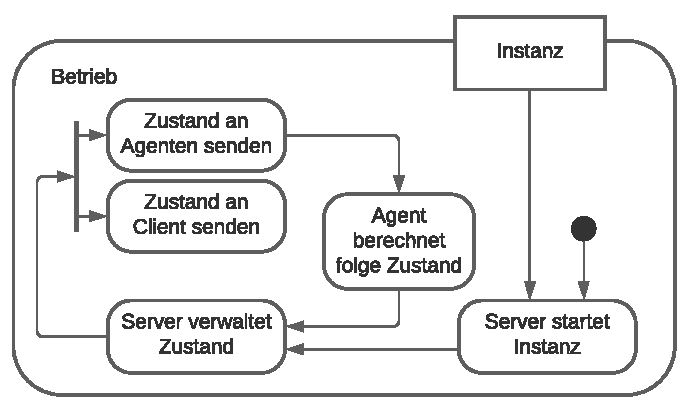
\includegraphics[scale=.65,center]{medien/top-down-betrieb}
%        \caption{Betrieb Ablauf Übersicht}
%        \ownsource
%    \end{figure}
%
%    Mit letzterem ergibt sich dann ein Zyklus, welcher für eine Echtzeit darstellung verwendet werden kann.
%    Durch diese Darstellung kann dann der Nutzer sowohl die Auswirkungen des Straßennetztes als auch das Verhalten des Agenten erkennen.
%
%    Die Anwendung soll als Client-Server Anwendung aufgeteilt werden damit der Server lange laufen kann, mehrer Nutzer auf die gleiche Instanz zugreifen können und Hardware verwendet werden kann welche besonders CPU-Leistungsstark ist.
%    Der Client kann hingegen nach Belieben gestartet werden und mit einer Instanz verbunden werden, dieser Client benötigt, im Gegensatz zu dem Server, eine GPU um die Darstellung des Zustandes zu beschleunigen.
%
%    Der Server ist dabei so zu konstruieren, dass er sich problemlos erweitern lässt, um mehrere Server-Instanzen auf unterschiedlichen Geräten zu nutzen und so die Berechnung zu beschleunigen.
%
%    Hinzu kommt das die gesamte Anwendung so konstruiert werden soll das man sehr leicht weitere Elemente für die Straßenmodellierung hinzufügen kann, so das sich die verschiedensten Szenarien modellieren lassen.

%    Darüber hinaus soll sie leicht erweiterbar sein in den folgendenen drei Aspekten.
%
%    Die Straßen Kacheln. Das


    \subsection{Bausteinsicht}

Durch die hier folgenden Kapitel soll eine Übersicht über die implementierten Komponenten, ihre Funktionalität und ihre Verbindung zueinander gegeben werden.

Diese ist allerdings nur als abstrakte konzeptionelle Übersicht zu verstehen und stellt nicht die vollständige Realität dar.
Die Notwendigkeit ergibt sich, da für die tatsächliche Implementation 44 Komponenten mit insgesamt 212 TypeScript Quellcode-Dateien erstellt worden sind, die sich hier unmöglich alle darstellen lassen.

Zusätzlich zu diesen sind noch drei externe Pakete entstanden, die auf grund der Übersichtlichkeit hier ebenfalls ausgelassen worden sind.

Für einen vollständigen Überblick sollte das Git Code Repository aufgesucht werden.
Einen Verweis zu diesem ist in Kapitel \refsec{sec:artefacts} zu finden.

Die nachfolgenden Kapitel sind anhand der unterschiedlichen Arten von Komponenten im Kontext der Parallelität von JavaScript gruppiert.
Zusätzlich wird diese Klassifizierung auch für die Komponenten-Diagramme benutzt.

Diagramm-Boxen repräsentieren Runtimes oder Worker bzw. den Main-Thread der Runtime.
Diagramm-Komponenten können Applications, Realms oder Realm Componentes darstellen, festgestellt werden kann dies über den Kontext des Abschnittes.

Die Diagramm-Komponenten in einem Application Kapitel, stellen Realms dar, in einem Realm Kapitel sind es dann wiederrum Realm Components und in einem Realm Components Kapitel können sie Dateien oder Klassen sein.

Das bedeutet auch, dass die Namen der Diagramm-Komponente aus den Application Kapiteln in Realm Kapiteln und die aus den Realm Kapiteln in Realm-Component Kapiteln beschrieben werden und durch sie assoziiert werden.

\subsubsection{Client Server Architektur}
\label{sec:client-server-arch}

Wie bereits in der Lösungsstrategie beschrieben, soll diese Anwendung als Client Server Anwendung realisiert werden.
Dadurch unterteilt sich diese Anwendung in zwei übergeordnete Komponenten.


\begin{figure}[htb]
    \centering
    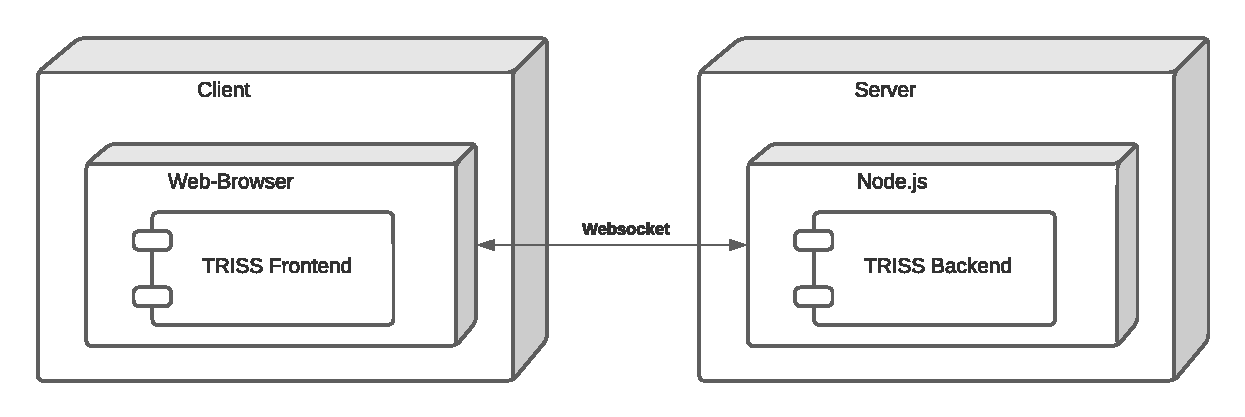
\includegraphics[scale=.65,center]{medien/client-server-start.pdf}
    \caption{Abstrakte Client Server Architektur}
    \ownsource
    \label{fig:abstract-client-server}
\end{figure}

\FloatBarrier

Der Client ist dabei das physikalische System, mit dem der Nutzer interagiert.
Auf diesem System muss ein moderner Webbrowser installiert sein, mit dem er das \highlight{TRISS Frontend} bezieht.
Das Frontend stellt dem Nutzer die Möglichkeit bereit, Server-Entitäten anzulegen und einzusehen.
Ebenfalls erlaubt er es, das Layout bzw. die Instanz via einer 3D-Darstellung zu erstellen und einzusehen.
Das Frontend Artefakt wird dabei durch einen statischen HTTP-Server bereitgestellt.

Das zweite Artefakt, das über den Server bereitgestellt wird, ist das \highlight{TRISS Backend}, das alle dynamischen Aktionen des Clients ermöglicht und gleichzeitig die Simulation bereitstellt.

Das Backend wird dabei im Gegensatz zu dem Frontend nicht via HTTP, sondern über das WebSocket-Protokoll angesprochen.
Der Vorteil besteht darin, dass dadurch das Backend nicht nur angesprochen werden kann, sondern auch Nachrichten ohne Anfrage an den Client senden kann.
Zusätzlich kommt die WebSocket-Verbindung, im Gegensatz zu HTTP oder Long-Polling\footnote{\url{https://javascript.info/long-polling}}, mit nur einer permanenten TCP-Verbindung aus\footnote{\url{https://datatracker.ietf.org/doc/html/rfc6455\#section-1.1}}.
Das reduziert nicht nur die Roundtrip-Zeit, sondern senkt auch zusätzlich den Berechnungs-Overhead, kontinuierlich neue TCP-Verbindungen aufzubauen.

Eine relevante Eigenschaft dieser Architektur ist, dass der Nutzer außer einem modernen Webbrowser keine weitere Software auf dem Gerät installiert haben muss, mit dem er die Anwendung verwalten will.
Es müssen nur das \highlight{TRISS Frontend} und das \highlight{TRISS Backend} vorher auf einem Server installiert worden sein.

Um die Inbetriebnahme weiter zu vereinfachen, werden beide Server Artefakte bzw. deren respektive Runtimes in zwei Docker Container verpackt.
Diesbezüglich folgen genauere Informationen im Kapitel \refsec{sec:distribution-view}.

\subsubsection{Application – TRISS Backend}
\label{sec:triss-backend-component}

Das TRISS Backend ist in drei Realms aufgeteilt.
Die zentrale Komponente ist die \highlight{Backend Server} Komponente, die als Single Source of Truth agiert und eingehende WebSocket-Verbindungen annimmt, Instanzen erstellt, deren Zustand verwaltet, die Erstellung von Agenten und Layouts erledigt und Frames zum Client schickt.

Allerdings produziert sie keine neuen Frames oder betreibt die Simulation, das erledigt die zweite Komponente, die \highlight{Worker Simulation Instance}.
Diese hat ein vergleichbar einfaches Interface, über das man die Welt und den Agenten setzen, die aktuelle Fahrzeugposition abfragen und die Simulation einen Schritt weiter laufen lassen kann.

Die dritte Komponente ist die \highlight{Worker Agent Sandbox} welche vom Backend Server dafür verwendet wird, um die Syntax und Interface Korrektheit eines neu erstellten Agenten zu prüfen.

Diese klare Aufteilung der Funktionen erlaubt es dann die \highlight{Worker Simulation Instance} als eigenen Worker auszuführen.
Dies wiederum hat einige Vorteile.
Der zentrale Vorteil ist, dass der Worker eine echte parallele Ausführung der Komponenten erlaubt und es somit möglich macht, eine Multicore CPU effizient zu verwenden.
Zusätzlich dazu, ist der Worker vom Server isoliert, wodurch der Agent schwerer den Server abstürzen lassen kann.
Auch kann der Worker so eigene globale Bibliotheken importieren und verwenden, ohne darauf achten zu müssen, dass diese nicht mit anderen Agenten oder dem Server kollidieren.

\begin{figure}[htb]
    \centering
    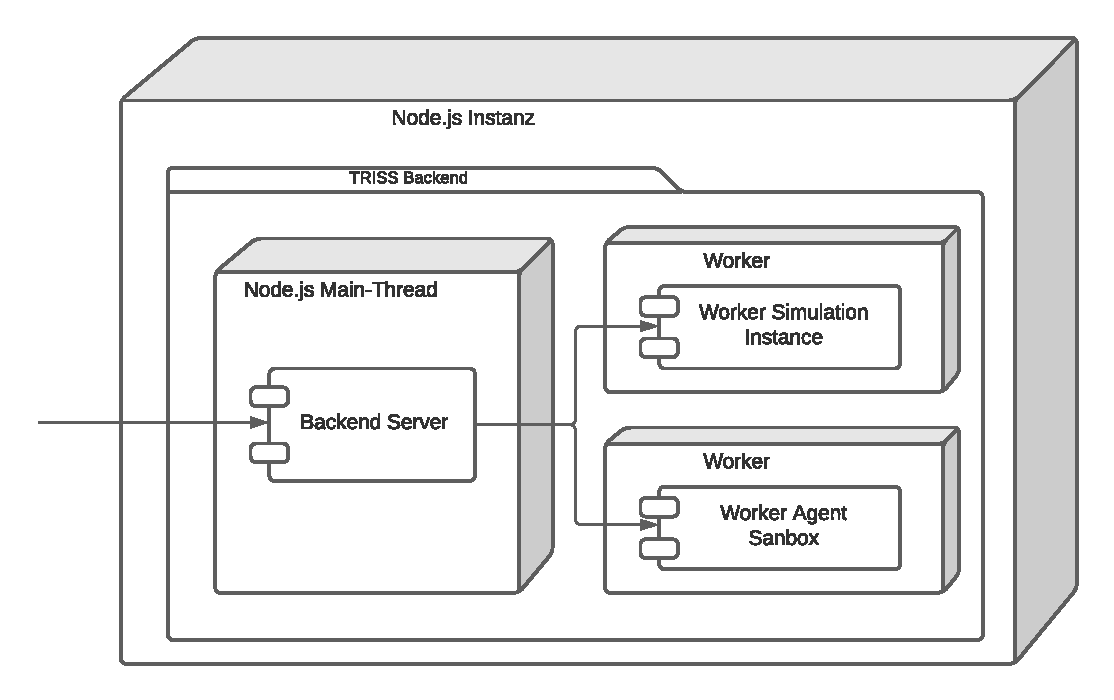
\includegraphics[scale=.65,center]{medien/triss-backend.pdf}
    \caption{Abstrakter Backend Server}
    \ownsource
    \label{fig:triss-backend}
\end{figure}

\FloatBarrier

Wie bereits beschrieben, hat JavaScript keine klassischen Threads, welche auf die gleichen Objekte zugreifen können.
Dieser Aspekt ist für diese Anwendung sehr relevant.
Denn damit ist die Isolation zwischen zwei Realms programmiertechnisch identisch zu der zwischen dem Node.js Server und der JavaScript Runtime des Browsers.
Das erlaubt es, alle Übertragungen gleichartig durchzuführen, ohne dabei unnötig Performance-Einbußen in Kauf zu nehmen.

Zusätzlich lassen sich die Komponenten identisch ansprechen, egal ob sie nun auf dem gleichen physischen System betrieben werden oder nicht.
Das bedeutet auch, dass sich der Server ohne größeren Auffand so erweitern lässt, dass er in einem Hardware-Cluster die Rechenlast verteilen könnte.
Es könnten aber auch beispielweise Agenten in einem Worker der Browser JavaScript Runtime ausgeführt werden, wenn dieser nicht Node.js spezifische Bibliotheken bzw. Schnittstellen braucht.

Dies bringt einen weiteren Vorteil mit sich, der hier ausgenutzt wird.
Dadurch kann nämlich der gleiche Serialisierungs-Algorithmus für alle Realm Übergänge verwendet werden sei es nun vom Backend Server zum Worker, vom Backend zum Frontend oder auch vom Backend zum Massenspeicher.
Dadurch ergibt sich ein weiterer sehr bedeutender Vorteil, so können Daten \enquote{getunnelt} werden, was hier durch die Worker bzw. durch den Backend Serve angewendet wird.

Wenn die Worker einen Frame, also einen diskreten Zustand, erzeugt haben, serialisieren sie diesen, mit dem Frame Serializer und schicken die Daten verpackt in ein Message Objekt an den Server.
Dieser packt das Message-Objekt aus, deserialisiert allerdings den Frame nicht, sondern verpackt diesen nur erneut in ein anderes Message-Objekt, das er an den Client schickt.
Dieser deserialisiert das vollständige Message-Objekt samt dem enthaltenen Frame und kann dann dort auf die hinterlegten Fahrzeuge zugreifen.

Für diese Aufgabe wurde im Kontext der Projektarbeit eine Bibliothek entwickelt, die vorgegebene Datenstrukturen in ein Binärformat um- und zurück wandelt.
Dieses Paket wurde \textit{serialization-generator}\footnote{\url{https://www.npmjs.com/package/serialization-generator}} genannt und via npm öffentlich zur Verfügung gestellt.
Auch wenn es andere Lösungen zur Serialisierung gegeben hätte, ist diese besonders an diese Verwendung angepasst, insofern sie auf die Benutzung mit TypeScript mit statischen Datenmodellen optimiert ist.

\subsubsection{Realm – Backend Server}

Der Backend Server ist die zentrale Komponente des TRISS-Backends.
Ihre Hauptaufgabe besteht darin, Verbindungen und Entitäten zu verwalten.

Zu diesen Verbindungen zählen die zu den Frontend Clients und den Worker Simulation Instances.
Die Menge der Entitäten enthält vor allem solche, die die Welt, den Agenten oder den aktuellen Simulationszustand in Form von Fahrzeugen repräsentieren.

\begin{figure}[htb]
    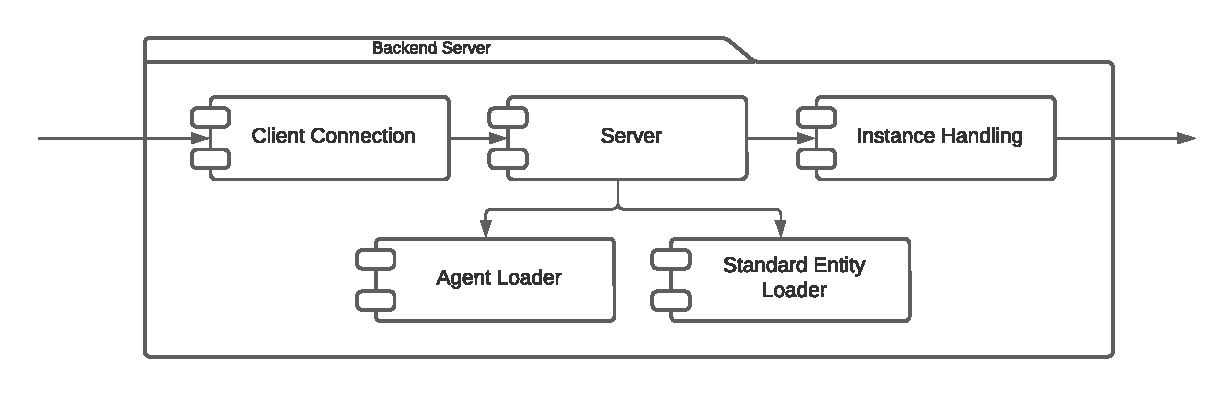
\includegraphics[scale=.65,center=\linewidth]{medien/backend-server.pdf}
    \caption{Backend Server}
    \ownsource
    \label{fig:backend-server}
\end{figure}

\FloatBarrier

Der Backend-Server ist der Realm, der alle Programmbestandteile zusammenbringt, Nachrichtenaustausch ermöglicht und Worker verwaltet.
Er leitet Nachrichten an die Clients weiter und ermöglicht Operationen auf den Entitäten auszuführen.

Dafür teilt er sich in fünf Komponenten, wobei alle bis auf den Server für die Kommunikations-Herstellung bzw. Entitäts-Bereitsstellung verantwortlich sind, und der Server diese nur verwaltet.
Dies repräsentiert sehr deutlich die Aufgabe dieses Realms.

\subsubsection{Realm – Worker Simulation Instance}

Der Worker Simulation Instance Realm beinhaltet die eigentliche Simulation und betreibt den dazugehörigen Agenten.
Um diese zu erledigen, besteht er aus drei Paketen.

\begin{figure}[htb]
    \centering
    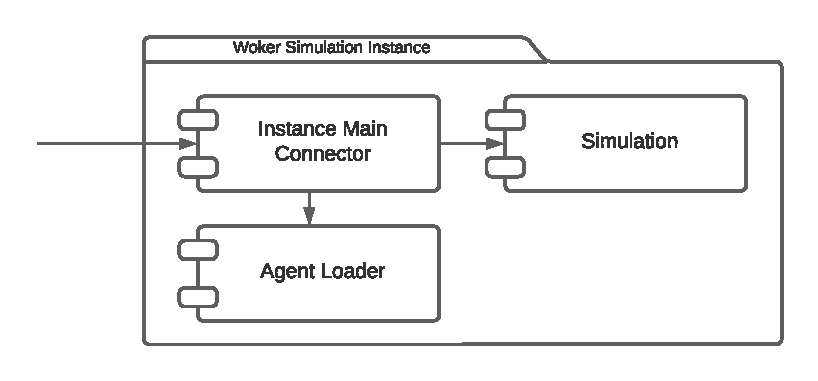
\includegraphics[scale=.65,center]{medien/worker-simulation-instance.pdf}
    \caption{Worker Simulation Instance}
    \ownsource
    \label{fig:worker-simulation-instance}
\end{figure}

\FloatBarrier

Der Realm ist insgesamt relative einfach gehalten und besitz ein kleines Interface um die Welt und die Agenten ID entgegenzunehmen, und diese dann weiterzuleiten bzw. zu laden und dann in Betrieb zu nehmen.

Die Worker Simulation Instance Komponente repräsentiert immer genau eine Simulationsinstanz und bleibt für die Komplette dauer der Lebenszeit der Instanz bestehen.

Sie wird durch Nachrichten gesteuert und übersetzt diese auf die Simulation.
Im Gegensatz zum Backend Server Realm hat sie eine bedeutend höhere CPU Auslastung, da sie nicht nur durch den Agenten die eigentliche Simulation errechnet, sondern auch die Frames serialisiert.

\subsubsection{Realm – Worker Agent Sandbox}

Die Sandbox wird dafür eingesetzt, neu erstellte Agenten, die vom Frontend empfangen worden sind, auf Syntax-Korrektheit und auf ihre Interface-Konformität zu prüfen.

Dies geschieht in einem eigenen Realm, damit bei Syntaxfehlern nicht der gesamte Server abstürzt.

\begin{figure}[htb]
    \centering
    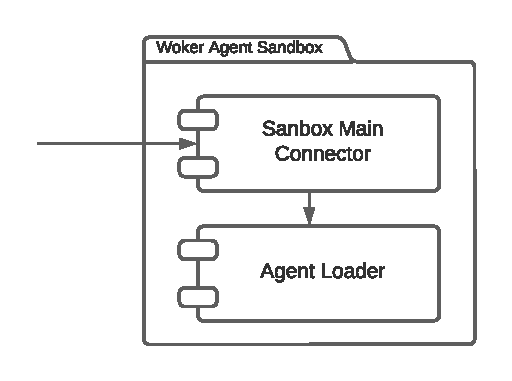
\includegraphics[scale=.65,center]{medien/worker-agent-sandbox.pdf}
    \caption{Worker Agent Sandbox}
    \ownsource
    \label{fig:worker-agent-sandbox}
\end{figure}

\FloatBarrier

Dafür benötigt er ebenfalls den Agent Loader, den er nach der Initialisierungsnachricht direkt verwende um den Agenten Testweise zu laden und so direkt prüfen zu können, ob das Laden erfolgreich ist, also alle Importpfade korrekt sind und die Syntax des JavaScript-Codes korrekt ist.

Wenn das gelungen ist, prüft er, ob alle Schnittstellen implementiert worden sind und liefert das Resultat wieder an den Main-Thread zurück.
Daraufhin wird er von außen wieder heruntergefahren.

\subsubsection{Realm Component – Server}

Die Server Komponente ist für den Backend Server Realm die verwaltende Kraft, alle anderen werden entweder von ihr angesprochen oder sprechen diese an.

\begin{figure}[htb]
    \centering
    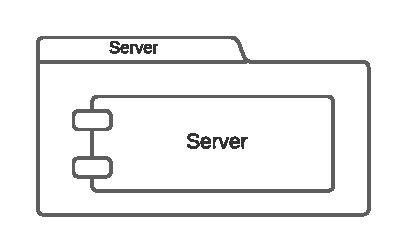
\includegraphics[scale=.65,center]{medien/server.pdf}
    \caption{Server}
    \ownsource
    \label{fig:server}
\end{figure}

\FloatBarrier

Sie verwaltet die Simulations-Instanzen, die Agenten und die Entitäten.
Diese Komponente wird bei der Ausführung des Servers als Singleton erstellt und bleibt bis zum Ende der Ausführung bestehen.

\subsubsection{Realm Component – Agent Loader}

Der Agent Loader ist von besonderer Bedeutung für den Server.
Er erlaubt es neue Agenten anzulegen und sie zu verwalten.

\begin{figure}[htb]
    \centering
    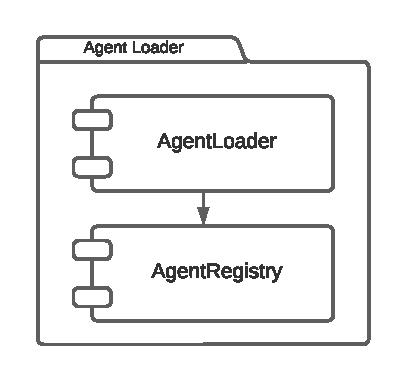
\includegraphics[scale=.65,center]{medien/agent-loader.pdf}
    \caption{Agent Loader}
    \ownsource
    \label{fig:agent-loader}
\end{figure}

\FloatBarrier

Durch die bereits aufgezeigte Eigenschaft, dass Realms vollständig voneinander getrennt sind, wird sie vor allem dafür eingesetzt, um den Agenten in dem Backend Server Realm zu speichern und dann im Worker Agent Sandbox und Worker Simulation Instance Realm wieder zu laden.
Deshalb muss sie gespiegelt in allen Realms des TRISS Backends erzeugt werden, jedoch werden jeweils unterschiedliche Funktionen von ihr verwendet.

Für die Bereitstellung hält er intern ein Register, was es ihm erlaubt Anfragen bezüglich der Liste von Agenten direkt zu beantworten, anstatt auf den Massenspeicher zugreifen zu müssen.

Nach dem Speichern liefert er eine ID zurück, welche dann vom Server verwendet wird, um auf diesen Agenten zu verweisen.

Geladen werden die JavaScript Sourcecode-Dateien über das ES-Module-System, als dynamischer import.
Dies erlaubt eine robuste und spezifikationskonforme Verwaltung und macht die Verwendung bzw. Implementation für den Nutzer vorhersehbarer und einfacher.

\subsubsection{Realm Component – Client Connection}

Die Client Connection Komponente bündelt alle Aspekte welche benötigt werden, damit der Client mit dem Server über das WebSocket Protokoll interagieren kann.

Eine der ersten Komponenten, die der Server dafür instanziiert, ist die WebSocket Server Klasse, die dann über den beigefügten TCP-Port auf neue Verbindungen wartet und dann, sollte er eine empfangen, eine Individual WebSocket Handler Komponente dafür erzeugt.

\begin{figure}[htb]
    \centering
    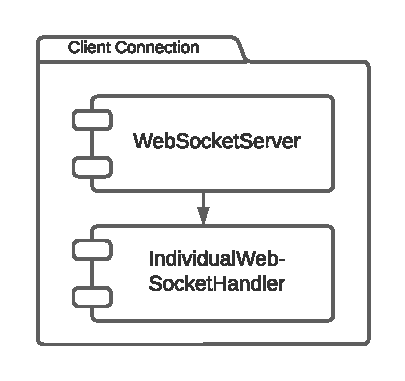
\includegraphics[scale=.65,center]{medien/client-connection.pdf}
    \caption{Client Connection}
    \ownsource
    \label{fig:client-connection}
\end{figure}

\FloatBarrier

Diese Komponente repräsentiert den individuellen Zustand der Client-Ver\-bindung, wie zum Beispiel welche aktuelle Instanz betrachtet wird.
Sie ordnet zentral die Anfrage-Nachrichten entsprechende Methoden Aufrufe zu und erzeugt die dazugehörigen Antwort-Nachrichten.

\subsubsection{Realm Component – Instance Handler}

\begin{figure}[htb]
    \centering
    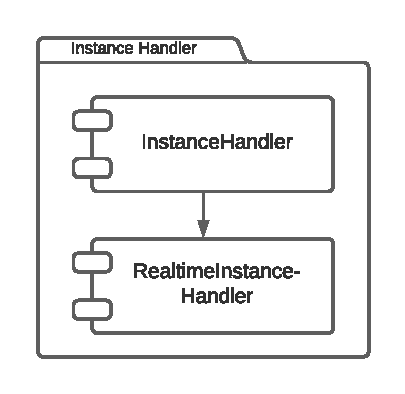
\includegraphics[scale=.65,center]{medien/instance-handler.pdf}
    \caption{Instance Handler}
    \ownsource
    \label{fig:instance-handler}
\end{figure}

\FloatBarrier

Der Simulation Instance Realtime Handler, ist die Komponente, die die Worker Simulation Instance Komponente verwaltet und als Repräsentant im Backend Server dafür einsteht.
Sie agiert ähnlich zu der Individual Web Socket Handler Komponente und übersetzt Methoden-Aufrufe zu Message-Objekten, die sie serialisiert und überträgt.
Zusätzlich beinhaltet sie Caches, damit beispielweise mehrere Individual WebSocket Handler auf den aktuellen Frame zugreifen können.

\subsubsection{Realm Component – Standard Entity Loader}

Der Standard Entity Loader wird vom Backend Server verwendet um dem Nutzer direkt eine kleine Auswahl an vorbereiteten Layouts und Agenten zur Verfügung zu stellen.

\begin{figure}[htb]
    \centering
    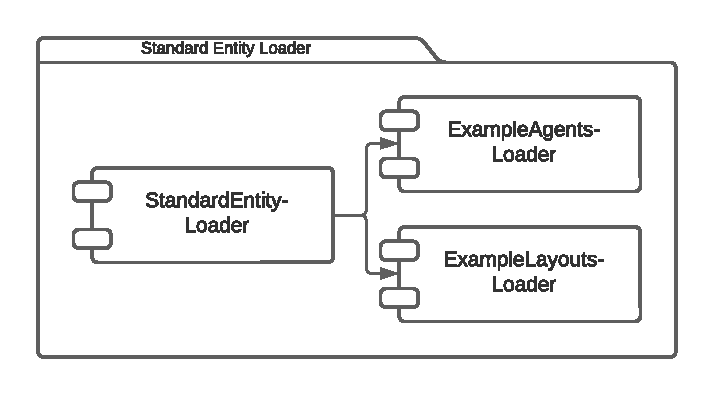
\includegraphics[scale=.65,center]{medien/standard-entity-loader.pdf}
    \caption{Standard Entity Loader}
    \ownsource
    \label{fig:standard-entity-loader}
\end{figure}

\FloatBarrier

Dafür wurden die Komponente so konfiguriert, dass sie eine statische Liste mit Einträgen laden und an den Server zur Registrierung übermittelt.

Besonders wichtig ist dabei das Laden des Random Exit Drivers, der als Beispiel Agent viele Aspekte für die Implementierung eines solchen demonstriert.

Die Standard-Layouts umfassen von einfachen manuell erstellen Layouts, welche die besonders groß sind, viele Routen zulassen, viele Kreuzungen beinhalten, viele Erzeugungs- und Zerstörungs-Punkte beinhalten und eines das Leer ist.

Diese sollen dabei unterstützen noch schneller mit der Entwicklung und dem Experimentieren beginnen zu können.
Zusätzlich können sie als Beispiel für die Entwicklung von komplizierteren Layouts benutzt werden und deren Implementationen inspirieren.

So wurde beispielweise ein auf dem Wave-Function-Collapse-Algorith-\linebreak mus\autocite{wfca2019} basierter Layout Generator erstellt, welcher ein guter Startpunkt sein kann, um eine organischeres Layout in der Größenordnung einer kleineren Ortschaft zu erzeugen.

\subsubsection{Realm Component – Simulation}

Die eigentliche Simulation besteht aus zwei Komponenten, die unabhängig vom Kontext, also ob sie nun von einem Worker verwendet werden oder nicht, so angesprochen werden sollten.
Dabei nimmt die Simulation Instance die verwaltende und kapselnde Rolle bezüglich der Simulation ein und abstrahiert welche Engine verwendet wird und wie diese konkret angesprochen wird.
Sie beinhaltet auch Meta-Informationen, wie beispielweise den Namen oder die ID der Simulation.

\begin{figure}[htb]
    \centering
    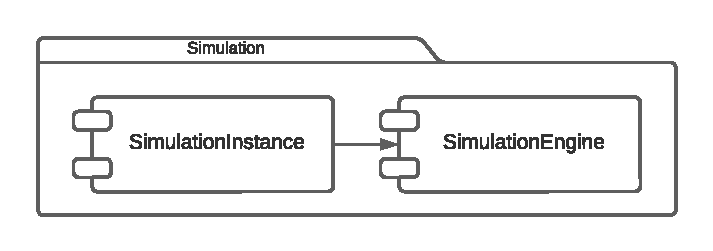
\includegraphics[scale=.65,center]{medien/simulation.pdf}
    \caption{Simulation}
    \ownsource
    \label{fig:simulation}
\end{figure}

\FloatBarrier

Die Engine ist das eigentliche ‚Herzstück‘, das die Simulation an sich vorantreibt.
Sie erhält über die Simulation Instance von dem Instance Main Connector den Agenten, den sie verwenden soll, um die Simulation zu betreiben.
Sie verwaltet intern alle notwendigen Zustände und spricht den Agenten mit diesen an.
Für den Agenten stellt sie die Schnittstelle zu dem restlichen System dar, insofern sie die einzige Referenz ist, die an den Agenten übergeben wird.

Hier bestünde die Möglichkeit, die Software zu erweitern, in dem andere Varianten der Engine entwickelt werden.
Diese könnte dann beispielweise eine andere Art von Agenten unterstützen, welcher lokal auf nur einem Fahrzeug agiert und dadurch direkt von der Engine multithreaded werden könnte.
Eine weitere Option wäre eine Engine, die andere Prozessschritte inkludiert, wie beispielweise eine Kollisionsberechnung als Validierungsschritt.

\subsubsection{Realm Component – Instance Main Connector}

\begin{figure}[htb]
    \centering
    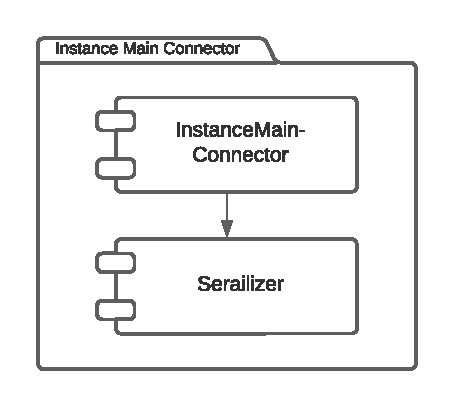
\includegraphics[scale=.65,center]{medien/instance-main-connector.pdf}
    \caption{Instance Main Connector}
    \ownsource
    \label{fig:instance-main-connector}
\end{figure}

\FloatBarrier

Das Instance Main Connector Paket stellt die Abstraktion bezüglich der Verwendung in einem Worker bereit und erlaubt die Verwendung der Simulation in dieser Konstellation.
Er stellt das Gegenstück zu dem Simulation Instance Realtime Handler aus dem Backend Server dar und tauscht mit diesem Nachrichten aus.
Er ist die einzige semantische Verbindung zum Gesamtsystem.

Er verwendet wie auch die anderen Realm-Übergänge die entsprechenden Serialisierer.


\subsubsection{Realm Component – Sandbox Main Connector}

Diese Komponente hat die gleiche Rolle wie der Instance Main Connector, nur für die Sandbox.

\begin{figure}[htb]
    \centering
    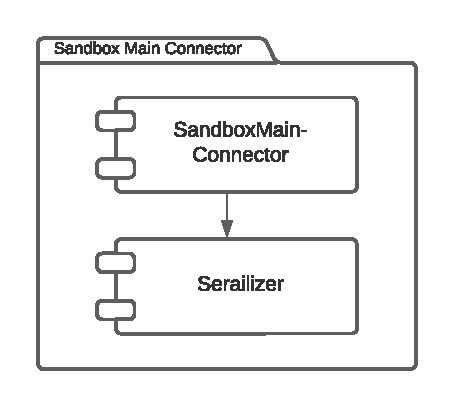
\includegraphics[scale=.65,center]{medien/sandbox-main-connector.pdf}
    \caption{Sandbox Main Connector}
    \ownsource
    \label{fig:sandbox-main-connector}
\end{figure}

\FloatBarrier

Im Gegensatz zu ihr, besitzt dieser jedoch andere Kommandos und verwendet selbst andere Komponenten.
Zusätzlich ist er anders gegen Fehler geschützt und liefert diese zurück an den Main-Thread, damit dieser diese Fehlermeldung wiederum an den Client geben kann und somit der Nutzer nachvollziehen kann, warum der Agent ggf. abgelehnt worden ist.

\subsubsection{Application – TRISS Frontend}
\label{sec:triss-frontend-component}

Das TRISS Frontend ist das zweite eigenständige Element der TRISS Anwendung.
Sie ist ein rein passives Element und enthält keine Anwendungslogik, sondern dient lediglich der Ansteuerung der Anwendung und Visualisierung der Simulation.

\begin{figure}[htb]
    \centering
    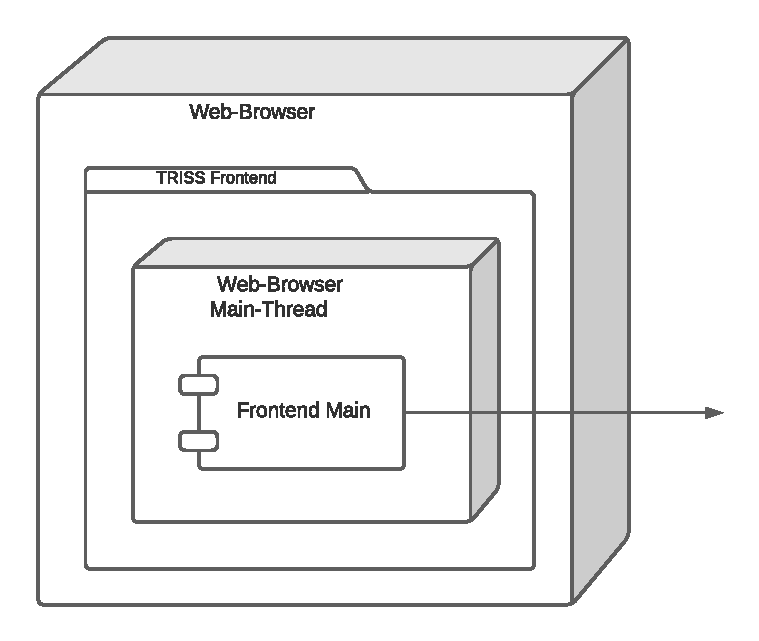
\includegraphics[scale=.65,center]{medien/triss-frontend.pdf}
    \caption{TRISS Frontend}
    \ownsource
    \label{fig:triss-frontend}
\end{figure}

\FloatBarrier

Sie besteht aus einem einzigen Realm, welcher die komplette Anwendung umschließt.
Neben dem JavaScript Realm betreibt das Frontend, wie im weiteren Verlauf erläutert, durch three.js eine WebGL Kontext, der hier jedoch nicht mit eingezeichnet ist.

\subsubsection{Realm – Frontend Main}

Der Frontend Main Realm, ist sehr umfangreich und teilt sie sich in vier Hauptkomponenten.

\begin{figure}[htb]
    \centering
    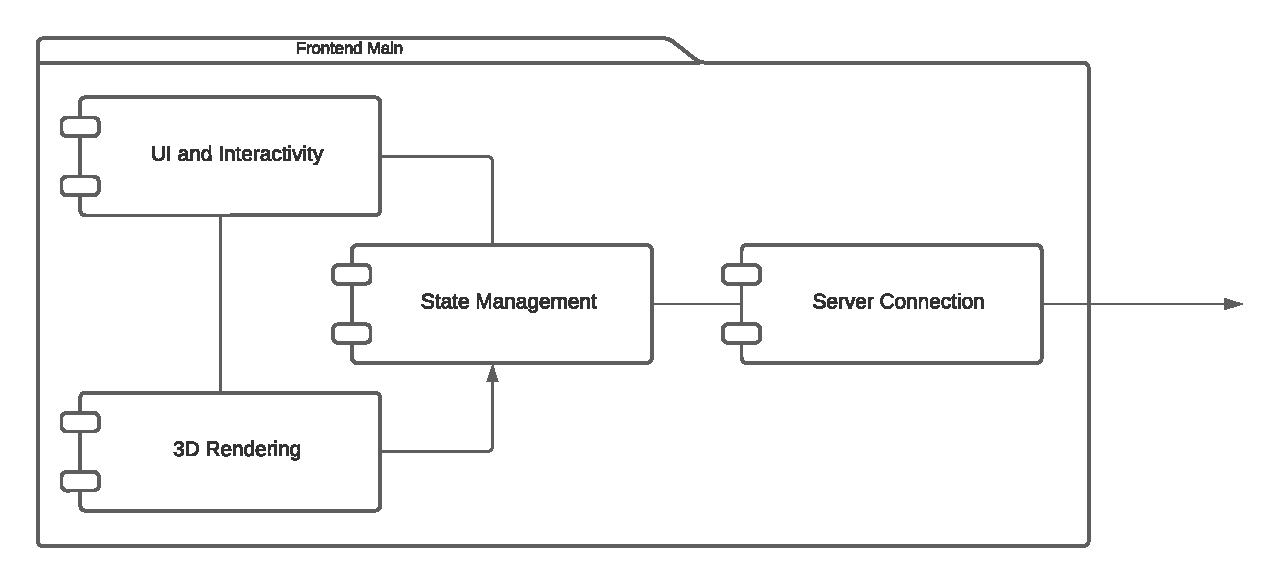
\includegraphics[scale=.65,center]{medien/frontend-main.pdf}
    \caption{Frontend Main}
    \ownsource
    \label{fig:frontend-main}
\end{figure}

Das zentrale Element dabei ist die State Management Komponente.
Sie vereint alle Aspekte rund um die Spiegelung der Server-Status als auch die Speicherung des UI-Zustands.
Sie dient als Single Source of Truth bzw. dessen Spiegelung.
Mit bzw. über diese Komponente kommunizieren alle anderen.
Es wurde versucht, die Anwendung so zu entwickeln, dass alle anderen Komponenten zustandslos sind.

Die Server Connection Komponente ist dabei der Counterpart der Individual WebSocket Connection Komponente und vereint ähnlich wie diese die De-/Serialisierung und das Abbilden von Methoden auf Nachrichten und umgekehrt.
Darüber hinaus ist sie auch dafür zuständig vom, HTTP-Server die Assets zu laden, da dies programmatisch und nicht vom Browser gesteuert wird.
Sie gibt alle erhaltenen Informationen an das State Management weiter und wird durch dieses bzw. dessen Events beauftragt, Daten einzuholen.

UI and Interactivity umfasst all die Aspekte des Frontends, mit denen der Nutzer interagieren und welche er sehen kann.
Sie stellt den Zustand dar, welchen das State Management aktuell hat, und meldet Ereignisse an dieses.
Diese Komponente befindet sich in einer Koexistenz mit dem 3D-Rendering, das auf Grundlage seiner Komplexität nicht mehr Teil der UI ist.
Diese Komponente bettet das 3D Rendering ein, liefert ihm den UI-Kontext und verarbeitet Events.

Die letzte, jedoch sehr zentrale Komponente, ist die 3D-Rendering-Kompo\-nente.
Diese umfasst, wie der Name andeutet, alle Aspekte bezüglich der drei dimensionalen Darstellung der Welt.
Sie ist als eine einzelne Komponente gefasst, da sie nur auf dem Parameter Welt beruht und somit ohne weiteres anderweitig verwendet werden könnte.
Des Weiteren ist sie bedeutend komplizierter und anders in ihrer Programmierung als die UI.

Die 3D-Rendering-Komponente ist, genauso wie die Datenübertragung und die Agenten, eine der Flaschenhälse, da sie direkt und in Abhängigkeit zur Menge der Fahrzeuge die Performance beeinflusst.
Deshalb wurde hier besonders auf die Implementation und deren Laufzeitverhalten Wert gelegt.

\FloatBarrier

\subsubsection{Realm Component – State Management}

Die Frontend Anwendung beruht zentral auf der Verwaltung des UI Zustandes.
Die größte Herausforderung, die bei der Entwicklung von Frontend Anwendungen anzutreffen ist, ist die Verwaltung des Zustandes der UI, der fachlichen Informationen und des Server Zustands.
Die Herausforderung tritt vor allem dann zutage, wenn versucht wird bei einer Frontend Anwendung Fehler zu finden, welche keinen Schwerpunkt auf die Zustandsverwaltung gelegt hat.
Diese Verwaltung hat demzufolge einen hohen Stellenwert erhalten und wurde in diesem Kontext zentral behandelt.

\begin{figure}[htb]
    \centering
    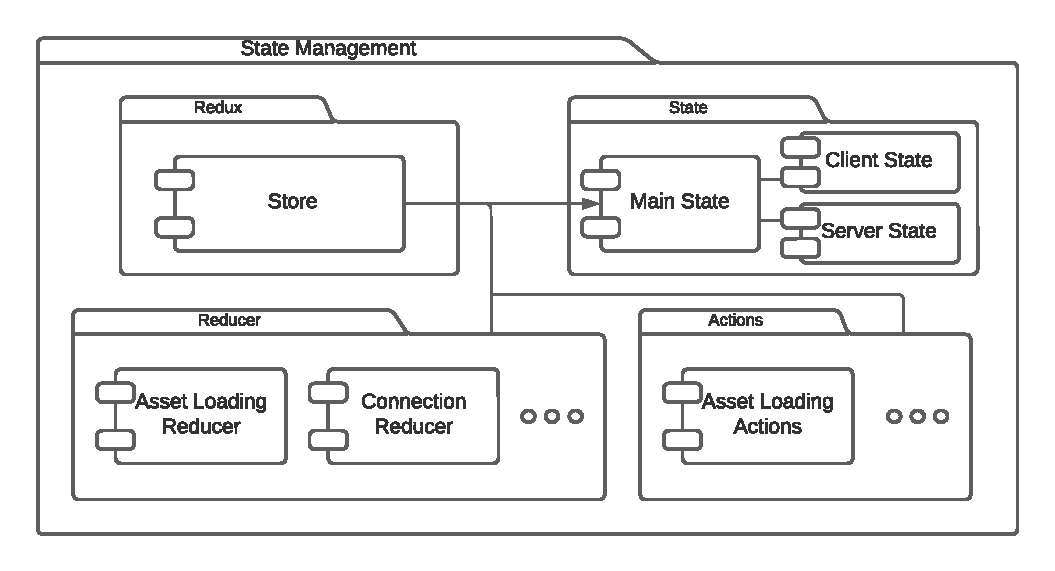
\includegraphics[scale=.65,center]{medien/state-management.pdf}
    \caption{State Management}
    \ownsource
    \label{fig:state-management}
\end{figure}

% \FloatBarrier

Da diese Aufgabe so zentral und typisch für das Frontend ist, bestehen dafür auch Standardlösungen.
Für diese Anwendung wurde sich für eine der am \helptex häufigsten verwendeten Lösungen\footnote{\url{https://2020.stateofjs.com/en-US/technologies/datalayer/\#datalayer_experience_ranking} (Es muss auf den \enquote{Usage} Reiter geklickt werden.)} entschieden, Redux.

Redux wird in dieser Anwendung als die zentrale Instanz für die Zustandsverwaltung verwendet.
Es handelt sich hierbei um eine verhältnismäßig einfache Bibliothek, die eher als Programmierkonzept anstatt als eine hoch komplexe technische Lösung angesehen werden sollte.
Es schreibt gewisse Verhaltensweisen bezüglich der Zustandsverwaltung vor, die, wenn man sie einhält, den Code bedeutend einfacher macht, viele Fehler vermeidet und es einem erlaubt die Anwendung bzw. deren Zustand über Werkzeuge zu analysieren und Fehler zu finden.

Diese Konzepte, die Redux vorschreibt, beziehen sich dabei konkret auf drei Arten von Komponenten, in die auch diese State Management Komponente aufgeteilt ist.
Das erste, das auch initial definiert werden muss, ist der Zustand der hier im Paket State enthalten ist.
Dabei handelt es sich um die Definition eines Objekt-Baumes, der für TRISS mit einem Main State als Wurzelknoten beginnt und dann den Client und den Server State beinhaltet.
Der Client State ist dabei der UI State und der Server State umfasst alle gespiegelten Daten vom Server, wie beispielweise welche Instanzen zur Verfügung stehen und welchen Frame als letztes von einer dieser erhalten worden ist.

Dieser Zustand wird von dem Redux Store gespeichert und verwaltet.
Der Zustand gilt als unveränderlich und wird nicht angepasst, sondern ersetzt, was im Kontext von JavaScript viele Fehler im Vorhinein verhindert und bedeutende Debugging-Möglichkeiten erschafft.
Um diesen Zustand zu ersetzen bedarf es sogenannte Reducer, die den aktuellen Zustand und die Action (ein Ereignis des Systems) als Parameter entgegen nehmen.
Aus diesen beiden Informationen erzeugt diese pure function\footnote{\url{https://en.wikipedia.org/wiki/Pure_function}} dann einen neuen Zustand, der den vorangegangenen ersetzt.

Diese Reducer enthalten also die UI bzw. Anwendungslogik.
Dadurch, dass sie pure sein müssen, der initiale Zustand bekannt ist und alle Events einfache Objekte sind, die man aufzeichnen kann, kann genau nachvollzogen werden, was zu dem aktuellen Anwendungszustand geführt hat.
Es lassen sich die Events auch wieder abspielen bzw. man kann auch zu einem vorangegangenen Zustand zurückspringen, wenn wie gefordert alle anderen Komponenten zustandslos sind und ihren Zustand im Store haben.

Die Actions sind die Ereignisse, die andere Komponenten senden können um eine Zustandsänderung herbeizuführen.
Diese Aktionen werden meist symmetrisch zu den Reducern definiert, insofern diese nur auf spezielle Actions reagieren.

\subsubsection{Realm Component – Server Connection}

Der Server Connector agiert ähnlich zu den anderen, bereits aufgezeigten Komponenten, die die Realm-Übergänge ermöglichen.
Der Server Connector des TRISS-Frontends unterscheidet sich allerdings insofern, dass er nicht nur die durch den serialization-generator erzeugten Nachrichten verarbeitet, sondern zusätzlich dazu noch HTTP-Nachrichten mit dem HTTP-Server austauscht, damit weitere Assets, wie beispielweise weitere Kacheln, geladen werden können.

\begin{figure}[htb]
    \centering
    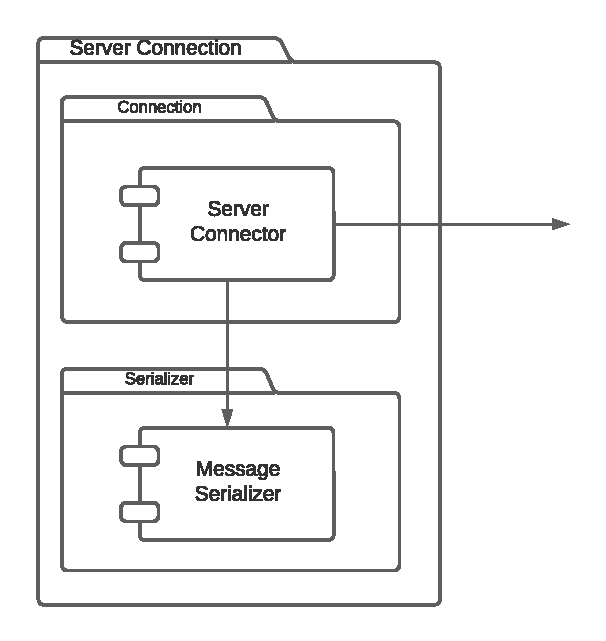
\includegraphics[scale=.65,center]{medien/server-connection.pdf}
    \caption{Server Connection}
    \ownsource
    \label{fig:server-connection}
\end{figure}

% \FloatBarrier

Er verwendet den gleich konfigurierten Serialisierer wie das TRISS Backend und verbindet sich mit diesem über das WebSocket Protokoll.
Das erlaubt es dem Backend, Frames zum Client zu übertragen, ohne dass dieser diese erst anfragen muss und automatisch über Änderungen am Server informiert wird, wie beispielweise, dass ein neuer Agent erstellt worden ist.

Diese Informationen leitet er via Actions an den Redux Store weiter.
Angesprochen wird er durch Reducer, die bei bestimmten Actions Anfragen an das Backend senden wollen.

\subsubsection{Realm Component – UI and Interactivity}

Die Komponente UI and Interactivity umfasst primär die React Komponenten.
Dadurch ist für diese React\footnote{\url{https://reactjs.org/}} die tragende Technologie.
Mit ihr lassen sich Funktionen definieren, die als Abbildungsfunktionen aufgefasst werden können, die einen konkreten Zustand in einen (Teil-)DOM übertragen.

Ein großer Vorteil von React ist, dass man die Benutzeransicht in einzelne deklarative Komponenten aufteilt, die man für sich genommen entwickeln und testen kann.
Übergeordnete Komponenten verwenden dann untergeordnete auf die gleiche Art und Weise wie man auch native HTML-Elemente gebrauchen würde.
Hinzu kommt das React durch den JSX bzw. TSX Syntax eine ausgesprochen übersichtliche programmierung erlaubt.

\begin{figure}[htb]
    \centering
    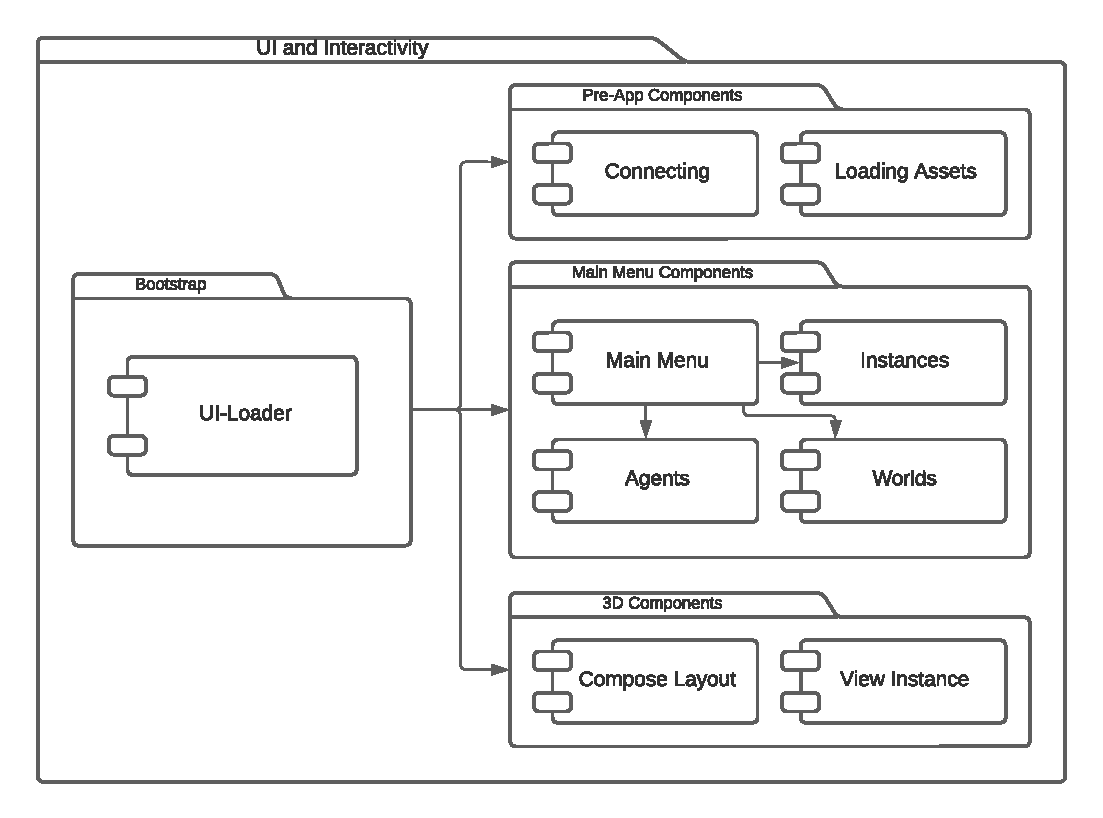
\includegraphics[scale=.65,center]{medien/ui-and-interactivity.pdf}
    \caption{UI and Interactivity}
    \ownsource
    \label{fig:ui-and-interactivity}
\end{figure}

% \FloatBarrier

Die Komponenten sind für die Darstelung in drei Gruppen unterteilt, welche ihren jeweiligen Schwerpunkt repräsentieren.
Zusammengebracht werden sie vom UI-Loader, der durch den im Store hinterlegten Pfad entscheidet, welche Komponenten aktuell geladen werden sollen.
Diese hängt er dann im DOM ein.
Dadurch rendert dann React diese Komponenten, wodurch dann via den React Hooks\footnote{\url{https://reactjs.org/docs/hooks-intro.html}} der aktuelle Zustand aus dem Redux Store gelesen wird und der Komponente zur Verfügung steht.

Diese erzeugt dann daraus den Pseudo DOM, der React mit dem realen abgleicht und wenn notwendig synchronisiert.
Nutzerinteraktionen werden via Events der Komponenten gemeldet, die diese in eine Action umwandelt und diese an den Store weitergibt.
Dieser verarbeitet dann, wie bereits beschrieben, diese Action mit Reducern, wodurch sich mit hoher Wahrscheinlichkeit der Zustand des Stores ändert und dadurch React die UI neu erzeugt.

Diese Komponenten haben also selbst keinen Zustand sondern spiegeln immer nur den Zustand wider, der im Redux Store enthalten ist.
Für die 3D-Components gilt zusätzlich das sie nur das UI für die 3D-Darstellung liefern, die 3D-Darstellung allerdings nicht übernehmen, sondern nur die DOM-Komponente für das Rendering in den DOM hängen.

\subsubsection{Realm Component – 3D Rendering}

Der 3D-Renderer ist das Herzstück des Frontends und hauptsächlich dafür verantwortlich, die von dem Server übertragenen Entitäten anschaulich darzustellen.
Um dies zu ermöglichen, wird hier sehr zentral mit der WebGL Schnittstelle des Browsers über die Bibliothek three.js gearbeitet.

Die Rendering Architektur ist dabei als Pipeline aufgebaut, da die Entitäten für die Darstellung mehrmals erweitert, zusammengefasst und gefiltert werden müssen.
Der Pipeline-Ansatz erlaubt es auch, neue Schritte einfach einzufügen und ganze Gruppen von Objekten zwischenzuspeichern, sollte sich herausstellen, dass sich die Eingabedaten in diesem Schritt nicht geändert haben.

So können neue Daten einfach am Anfang der Pipeline angelegt werden und die Änderungen kaskadieren dann bis zur eigentlichen Szenebildung mit Objekten, die three.js wiederum in Speicherstrukturen umformt, die durch WebGL verarbeitet werden können.

Zusätzlich erlaubt diese Struktur es, diese 3D-Darstellung in Zukunft einfacher zu parallelisieren,
auch wenn dafür vorher sichergestellt werden muss, dass der Overhead der De-/Serialisierung der Daten nicht größer ist als die eigentliche Umformung.

\begin{figure}[htb]
    \centering
    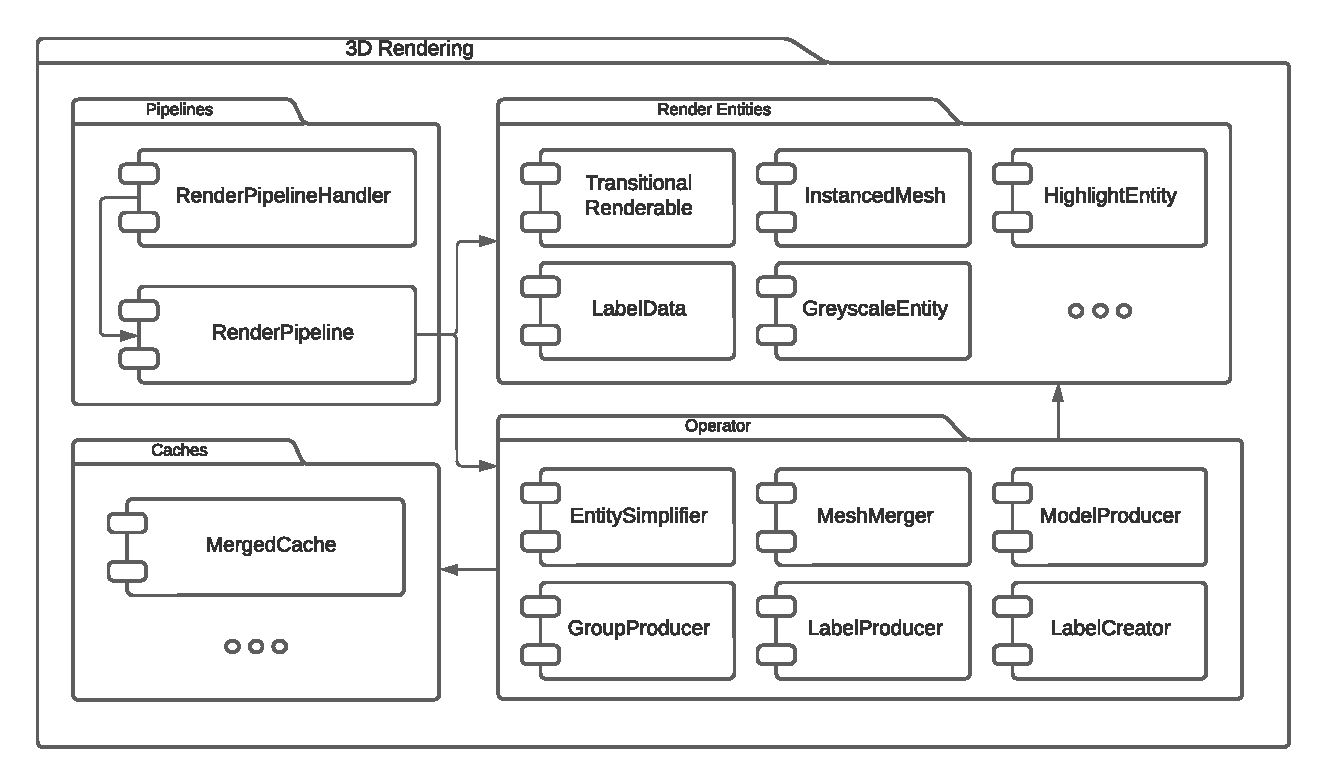
\includegraphics[scale=.65,center]{medien/3d-rendering.pdf}
    \caption{3D Rendering}
    \ownsource
    \label{fig:3d-rendering}
\end{figure}

% \FloatBarrier

Die 3D-Darstellung teilt sich dabei konkret in vier Pakete auf.
Das Operator Paket ist dabei das, das die eigentliche Funktionalität ermöglicht, indem es atomare Aktionen der Verarbeitung bereitstellt.
Diese Schritte umfassen Aufgaben, bei denen aus einer oder mehreren Eingabemengen eine oder mehrere Ausgabemengen erzeugt werden.

Beispielweise wird durch den Entity Simplifier aus der Positionsangabe, seiner Rotation und dem Typen der Entität das eigentliche 3D-Modell geladen bzw. erzeugt
und die Welt-Matrix berechnet, die seine Position widerspiegelt.

Der Mesh Merger hingegen ist dafür zuständig, aus einer Menge von Transitional Renderable Objekten Instanced Meshes zu erzeugen, die vom Shader Programm, das three.js bereitstellt, verarbeitet werden können und besonders effizient sind.

Alle Operatoren greifen dabei auf unterschiedlichste, auch teilweise verkettete Caches zu.
Diese Caches erlauben die Wiederverwendung von bereits erzeugten Objekten bzw. deren konkreten Konfigurationen.

Als Beispiel ist hier der Marked Cache anzuführen, der sich vor allem dadurch auszeichnet, dass er Einträge markiert, die in diesem Renderzyklus noch nicht verwendet worden sind.
Das erlaubt es, den Cache auch wieder zu entleeren, sodass dieser auch bei langanhaltender Verwendung nicht vollläuft und die Anwendung zum Absturz bringt.

Die Operatoren werden jedoch nicht direkt verwendet, da sie so noch keinen Nutzen haben.
Ihre eigentliche semantische Funktionalität wird erst durch die Render Pipeline erzeugt.
Diese nutzt die atomaren Operatoren, verknüpft sie und definiert, welche Daten in welchen Operator und in welchem Schritt geleitet werden sollen.

Diese Pipeline ist dafür gedacht, die dynamischen Entitäten, die durch den Agenten bzw. den Server definiert werde, in ihre respektiven (Teil-)Szenen\-graphen zu überführen.
Dies allein reicht jedoch nicht aus, um sie darstellen und mit ihnen interagieren zu können.
Diesen Anteil stellt der RenderPipelineHandler bereit.
Dieser erzeugt neben der Bodenplatte, dem Sonnenlicht und dem Firmament auch die Controller, die Nutzereingaben wie panning, zoom und click ermöglichen.

Zusätzlich macht er es sehr einfach, den Zustand der Welt zu aktualisieren.
Er ist die primäre und im Rahmen dieser Anwendung die einzige Komponente, die außerhalb des 3D-Moduls verwendet wird.


    \subsection{Laufzeitsicht}

In dem hier folgenden Kapitel soll dargestellt werden, welche Aktionen das System ausführt, um seine Funktionen bereitzustellen.
Dies erlaubt es, einen anderen Blickwinkel und damit ein besseres Verständnis für diese Anwendung zu erlangen.

Zu diesem Zweck wurden drei konkrete Abläufe ausgewählt.

\subsubsection{Anlegen eines neuen Agenten}

Der erste hier aufgeführte Fall soll beschreiben, welche Aktionen durchgeführt werden, um einen neuen Agenten anzulegen.

\begin{figure}[htb]
    \centering
    \includegraphics[scale=.65,center]{plant-diagrams/agent-creation-client-start.pdf}
    \caption{Client seitige Aktionen zum Anlegen eines Agenten}
    \ownsource
    \label{fig:agent-creation-client-start}
\end{figure}

Dabei beginnt der Ablauf mit dem Nutzer, der die Dateien auswählt, die seinen Agenten umfassen.
Die Dateien, die der Nutzer bereitstellt, sollen im Format eines npm-Paketes\footnote{\url{https://docs.npmjs.com/about-packages-and-modules}} sein.
Dies meint konkret, dass es im Wurzelverzeichnis eine package.json-Datei gibt, die neben der Version, dem Namen und der Beschreibung auch den Pfad zur Einstiegsdatei definiert.
Die dadurch festgelegte Einstiegsdatei ist der zweite erforderliche Bestandteil und muss eine kleine, aber zwingend erforderliche API implementieren.
Näheres dazu folgt in Kapitel \refsec{sec:artefacts}.

Zusätzlich kann er durch die package.json-Datei auch noch externe Abhängigkeiten definieren, die der Agent benötigt.
Diese werden dann bei der Installation mit installiert.

Alle bereitgestellten Dateien werden in Schritt \textbf{2.1} dann als Nachricht gebündelt.
Im Anschluss wird diese Nachricht dann an den Server gesendet.

\begin{figure}[tbp]
    \centering
    \includegraphics[scale=.65,center]{plant-diagrams/agent-creation-server.pdf}
    \caption{Der Server prüft den Agenten }
    \ownsource
    \label{fig:agent-creation-server}
\end{figure}

%\FloatBarrier

Dabei beginnt dieser mit der Prüfung der Daten und der Struktur in Schritt \textbf{3.1}.
In diesem Schritt wird vor allem sichergestellt, dass alle Informationen vorhanden und korrekt sind.
So wird beispielweise sichergestellt, dass der Name eine Mindestlänge hat und die angegebene Einstiegsdatei vorhanden ist.

Im Anschluss wird das Paket installiert.

Dafür werden im Zuge von Schritt \textbf{3.2} die mitgelieferten Dateien im Dateisystem abgelegt.
Dies ist notwendig, weil der ECMAScript-Standard in diesem Kontext keine synthetischen (in memory) Imports erlaubt und somit diese Dateien nur als ES Modules geladen werden können, wenn sie als Dateien vorhanden sind.

Idealerweise könnte man hier in der Zukunft einen, für diesen Zweck angepassten, ES Module Loader schreiben, welcher die Datei Inhalte im Arbeitsspeicher hält und diese direkt aus diesem laden kann.

Nach dem Schreiben ins Dateisystem wird er via Yarn im Schritt \textbf{3.3} installiert.
Damit sind dann seine Abhängigkeiten vorhanden und andere Pakete, wie der Agent Loader, können ihn referenzieren.

Hiernach wird versucht, den Agenten zu laden.

Dabei wird erst im Schritt \textbf{3.4} durch den Agent Loader eine Test-Sandbox (als Worker) mit dem Prüfscript geladen.
Diese erhält in \textbf{3.5} als Parameter die für den zu testenden Agenten vergebene ID.

%\FloatBarrier

Die Sandbox verhindert, dass der Server durch geladene Scripte oder durch Syntaxfehler leicht zum Absturz gebracht werden kann, und isoliert zusätzlich Fehlerquellen.

Durch das Installieren des Paketes kann dies hier nun durch die Namensreferenz aufgelöst werden und die Einstiegsdatei lässt sich durch einen asynchronen ES-Module import laden.

Durch das Laden prüft die Runtime implizit, ob der JavaScript-Code Syntaxfehler beinhaltet und ob alle Abhängigkeiten vorhanden sind.
Ebenso wird dadurch jeglicher Code ausgeführt, der nicht als Funktion verpackt worden ist.

Anschließend wird, falls das erfolgreich ist, im Schritt \textbf{3.11} geprüft, ob der Agent die notwendigen API Exports aufweist.
Dies soll vor allem dabei helfen, schnell strukturelle Fehler aufzudecken.

Sollte es hierbei zu Problemen gekommen sein, wird eine entsprechende Fehlermeldung generiert und an den Server bzw.
den Agent Loader zurückgegeben.

Im Diagramm wird der positive Fall dargestellt und das Erstellen eines Agenten ist somit mit \textbf{4.1} abgeschlossen.
In einem Fehlerfall würden nach \textbf{3.9} noch die umgekehrten Schritte bezüglich \textbf{3.2} und \textbf{3.3} folgen.

\begin{figure}[htb]
    \centering
    \includegraphics[scale=.65,center]{plant-diagrams/agent-creation-client-end.pdf}
    \caption{Der Client erhält die Antwort und stellt diese dar}
    \ownsource
    \label{fig:agent-creation-client-end}
\end{figure}

Durch den Socket wird dann die Rückmeldung an den Client gesendet.
Diese stellt der Client dann für den Nutzer dar.
In dem Diagramm \refgoal{fig:agent-creation-client-end} ist der positive Fall dargestellt.

Hierbei ist es wichtig, dass der Client durch diese Rückmeldung ebenfalls die Übersicht über die Agenten erweitert und dem Nutzer so darstellt, dass das Anlegen erfolgreich war.

\subsubsection{Erzeugung einer Instanz}

Als zweiten Anwendungsfall soll dargestellt werden, wie eine Instanz erzeugt wird, da dieser Ablauf zusätzlich hilft, ein besseres Verständnis hinsichtlich der Funktionsweise der Anwendung zu erlangen.

Das Erzeugen einer Simulationsinstanz besteht im Kern aus drei Abschnitten, bei denen vor allem Abschnitt eins uns drei nahezu identisch zu denen aus dem vorangegangenen Ablauf sind und deshalb hier nicht noch einmal wiederholt werden sollen, sondern nur kurz beschrieben werden.

Abschnitt eins beinhaltet auch hier die Nutzerinteraktion, bei der dieser das Straßennetz und den Agenten auswählt.
Zusätzlich vergibt er auch hier einen Namen und optional eine Beschreibung.
Der Client erzeugt dann daraus eine Nachricht, serialisiert diese und sendet sie an den Server.

Abschnitt drei verhält sich ebenfalls ähnlich und stellt das Erzeugungsresultat dem Nutzer dar.

Der zweite Abschnitt unterscheidet sich jedoch und beinhaltet die eigentliche Aktion des Systems, wie in dem folgenden Diagramm gezeigt werden soll.

\begin{figure}[htb!]
    \centering
    \includegraphics[scale=.65,center]{plant-diagrams/create-sim-main.pdf}
    \caption{Erstellung Simulationsinstanz, Server Thread}
    \ownsource
    \label{fig:create-sim-main}
\end{figure}

%\FloatBarrier

Beginnend mit dem Erhalt der Nachricht, fängt der Server an, die Aufforderung zur Erzeugung zu verarbeiten.
Um diese zu beantworten, beginnt der Server damit eine Liste aller Agenten und dann aller verfügbaren Layouts zu erzeugen.

Danach prüft er, ob er die IDs für das Layout und den Agenten in diesen Listen findet.
Sollte das der Fall sein, erzeugt er eine Simulation Instance, die in diesem Fall einen Realtime Handler hat.

Dieser Handler beinhaltet in seinem Konstruktor die Anweisung, einen neuen Node.js Worker zu erzeugen.
Sobald dieser erzeugt worden ist, wird eine Nachricht gesendet, die diesen Einstiegspunkt anweist, die eigentliche Instanz zu erstellen.

Schritt \textbf{4.1} ist also nur für die Node.js Worker verantwortlich und \textbf{4.2} beinhaltet die notwendigen Informationen für die eigentliche Simulationsinstanz.

Darunter befindet sich vor allem die Konfiguration des Agent Loaders, die ID des Agenten und das initiale Layout, das nicht als ID, sondern als World Objekt übertragen wird.

Auch diese Nachricht wird, wie auch die Nachrichten, die an den Client gesendet werden, mit den gleichen Werkzeugen serialisiert.
Dies wird hier zur Übersichtlichkeit nicht gezeigt, ist aber für die Anwendung relevant, um die notwendige Geschwindigkeit aufrechtzuerhalten.

Danach beginnt der Instance Main Connector mit der Verarbeitung, was in der folgenden Abbildung dargestellt werden soll.

\begin{figure}[htb]
    \centering
    \includegraphics[scale=.65,center]{plant-diagrams/create-sim-worker.pdf}
    \caption{Erstellung Simulationsinstanz, Worker Thread}
    \ownsource
    \label{fig:create-sim-worker}
\end{figure}

%\FloatBarrier

Hierbei wird der Instance Main Connector durch die Erzeugung des Workers automatisch instanziiert.
Im Anschluss wartet dieser auf das Instanzerzeugungs-Kommando, das die oben genannten Informationen enthält.

Durch diese kann er dann den Agent Loader erzeugen und mit diesem dann den Agenten anhand seiner ID laden.

Im Anschluss wird aus den Informationen, die übertragen worden sind, eine Welt erzeugt.
Diese Erstellung inkludiert vor allem die Instanziierung der Klassen, denn die übertragenen Objekte haben keine Assoziationen mehr mit diesen.

Danach wird in Schritt \textbf{5.7} die tatsächliche Simulations-Instanz erzeugt.
Sie steuert den Agenten an und verwaltet den Weltzustand.

Durch sie kann später ein neuer Frame angefragt werden.
Die Instance Main Connector Klasse so wie die Simulation Instance Realtime Handler Klasse könnte beide vernachlässigt werden und die Simulation Instance könnte direkt von dem Server angesprochen werden, sollte man keine Isolation oder Multithreading verwenden wollen.

Sollte diese Erzeugung funktioniert haben, dann meldet der Instance Main Connector nun den Ready Status zurück.
Daraufhin trägt der Server diese Instanz in seinem Register ein und meldet die neue ID der Instanz an den Client zurück.

In diesem Zustand könnten nun Frames von dem Handler bzw. der Simulation Instance angefragt werden.

\FloatBarrier

\subsubsection{Der Frame-Passthrough}

\newcommand{\processbegin}[2]{\item[$\mapsto$] \textbf{\textit{#1} #2:}}
\newcommand{\processstep}[2]{\item[$\rightarrow$] \textbf{\textit{#1} #2:}}

Der Frame-Passthrough umfasst alle Schritte, die notwendig sind, um durch das initiale Zeitgeber-Signal einen Pixel-Buffer zu füllen.

Für diesen sollen die übergreifenden Prozesse nur kurz textuell beschrieben und ausschließlich der Entitätsumformungsprozess im Detail beleuchtet werden.

Zentral zu beachten ist, dass der Prozess der Darstellung und der Berechnung der Frames bei dieser Anwendung voneinander getrennt sind und parallel zueinander laufen.
Verbunden sind diese Prozesse durch die Synchronisation des Zustandes der Welt sowie die zeitliche Synchronisation durch die Bildwiederholrate.

Somit muss unterschieden werden, welcher Prozess betrachtet wird.
Sie werden daher hier auch getrennt voneinander beschrieben.

Begonnen werden soll mit dem des Servers.
Dieser hat im Grunde einen sehr einfachen Zyklus, der hier Schritt für Schritt aufgelistet werden soll.

Jeder Stichpunkt repräsentiert einen Schritt und dieser ruft den nächsten auf bzw. leitet an ihn Daten weiter.

\textit{SR} = Backend Server Realm, \textit{WR} = Worker Simulation Instance Realm

\begin{itemize}
    \processbegin{SR}{Frame Loop 60 Hz Signal} Begonnen wird bei der Frameloop, die 60 Mal die Sekunde ein Signal sendet.

    \processstep{SR}{Simulation Instance Realtime Handler} Der Realtime Handler, der auch den Timer beinhaltet, woher auch sein Name stammt, nimmt dieses Signal auf und leitet es an seinen Worker weiter.
    Zusätzlich erneuert er interne Caches und benachrichtigt im Anschluss zu der Frameerzeugung alle Event Listener.

    \processstep{SR}{Simulation Instance Message Serializer} Diese Serialisierungs-Einheit formt die JavaScript-Werte und Objekte in ein Binärformat um, damit sie transferiert werden können.
    Dieser Schritt wäre nicht gezwungenermaßen notwendig, insofern der interne Serialisierer dies sonst machen würde, jedoch erlaubt dieser, die Werte direkt serialisiert weiter an den Client zu reichen und nicht im SR später erneut serialisieren zu müssen.

    \processstep{WR}{Simulation Instance Message Serializer} Dieser Serialisierer ist das entsprechende Gegenstück und wird vor allem zum Serialisieren der Frames benötigt.

    \processstep{WR}{Instance Main Connector} Die Komponente ist in dem Kontext der Verwendung des Workers geschrieben worden.
    Sie baut die Verbindung zu dem Server Thread auf und verwendet den Serialisierer.
    Nach der Instanziierung erwartet sie die Initialiserung-Nachricht und erlaubt im Anschluss das Anfragen neuer Frames.
    Sie schirmt den Verwendungskontext bezüglich der Simulation Instance ab.

    \processstep{WR}{Simulation Instance} Diese Komponente ist die Fassade für die eigentliche Simulation.
    Sie beinhaltet Methoden, die das Verwalten vereinfachen und erhält das durch den Instance Main Connector erhaltene Signal in Form von Aufrufen der \textit{calculateNextFrame} und \textit{getCurrentFrame} Methoden.

    \processstep{WR}{Simulation Engine} Die Simulation Instance hat das Ziel die Verwendung für den Client bzw.
    deren kumulierte Anfragen zu beantworten.
    Im Gegensatz dazu ist die Simulation Engine mehr low level und hat im Grunde nur Getter und Setter so wie die Frame Iterationslogik.
    Sie verwalten auch den Agenten und sie ist der beabsichtigte Weg diesen zu verwenden.

    \processstep{WR}{Agent} Der Agent ist die Instanz, die durch die Simulation Instance erzeugt worden ist.
    Der Agent wird durch den Konstruktor, der in den Agenten-Dateien definiert worden ist, erzeugt und erhält dabei Kontextinformationen sowie eine Referenz zu der Simulation Instance, die ihn erzeugt hat.
\end{itemize}

Ab dem Agenten lässt sich die Nachverfolgung des Frame Signals nicht fortführen, da sich die nach folgenden Schritte nicht generalisieren lassen.
Im Fall des Beispielagenten, der im Rahmen dieser Arbeit entwickelt worden ist, werden innerhalb des Agenten dann zuerst alle freien Spawn Plätze belegt und dann im Anschluss alle Fahrzeuge synchron, wenn möglich, bewegt.

Unabhängig von diesem internen Ablauf wird, wenn der Agent eine neue Welt zurückgeliefert hat, dieser Ablauf rückwärts ausgeführt.
Der Realtime Handler benachrichtigt dann alle eingetragenen Listener.
Diese stammen aus Clients, die über den aktuellen Zustand dieser speziellen Instanz benachrichtigt werden möchten.

Der Client als solcher läuft zu diesem Ablauf parallel.
Dieser hat dafür einen eigenen Zeitgeber, damit die Darstellung für den Nutzer flüssig bleibt.

Sollte ein Client registriert sein, erhält er durch den folgenden Ablauf den aktuellen Weltzustand.

\textit{SR} = Backend Server Realm, \textit{MR} = Frontend Main Realm, \textit{GT} = Graphics Thread

\begin{itemize}
    \processbegin{SR}{Instance Changed Event} Dies ist das Event, das durch die Rückmeldung vom Worker Thread zustande kam.

    \processstep{SR}{Simulation Instance Realtime Handler} Es wird vom Simulation Instance Realtime Handler angenommen und für Caches verarbeitet.
    Im Anschluss ruft dieser alle auf ihm registrierten Listener auf.

    \processstep{SR}{Individual WebSocket Handler} Dieser Handler hatte sich, durch die Client Nachricht cm-start-sending-frames bei der Simulations-Instanz für Veränderungen angemeldet.
    Er formt das Event nun um und sendet es weiter.
    Dabei muss der Frame nicht erneut serialisiert werden, da er noch serialisiert im Speicher liegt.
    Er kann bei allen WebSocket Handlern einfach in eine entsprechende Nachricht verpackt werden was enorm Ressourcen spart und den Server Thread responsiv hält.

    \processstep{SR}{Client-Server Partial Serialiser} Der Partial Serialiser, so genannt, weil er den Frame nicht serialisiert, serialisiert auch hier die Nachricht und sendet sie in einem minimal Binärformat an den Client über das WebSocket Protokoll.
    Dieses erlaubt einen bidirektionalen Nachrichtenaustausch und hilft somit bei der latenzarmen Frameübermittlung.

    \processstep{MR}{Client-Server Serialiser} Der Client Serialiser entpackt die Nachricht nun vollständig samt dem Frame und erzeugt wieder JavaScript Values.
    Diesen neuen Frame hängt er einer Redux Action an und dispatched diese auf dem Store.

    \processstep{MR}{Redux Store/Reducer} Der Store leitet diese dann weiter an den received-frame Reducer, der einen neuen Store-Zustand erzeugt, was wiederum alle Store-Subscriber benachrichtigt.

    \processstep{MR}{Simulation State Controller} Der State Controller ist die Einheit, die durch das React Element erzeugt wird und die übergeordnete Verbindung zwischen React, Redux und der Render-Pipeline herstellt.
    Er wird bei Frame-Änderung benachrichtigt und gibt den Frame an den Renderer weiter.
    Zusätzlich wird er auch in die Animation Loop eingebunden und erlaubt das Selektieren von Entitäten.

    \processstep{MR}{Render Pipeline Handler} Dies ist der Handler, der das eigentliche Rendering übernimmt.
    An ihn wird der Frame übergeben, den er speichert und dann die Frame dirty Flag setzt.
\end{itemize}

Nun sind der aktuelle Frame sowie alle weiteren notwendigen Informationen im Renderer hinterlegt.
Dieser hat, wie bereits angemerkt, seinen eigenen Zeitgeber, der von der Bildwiederholrate des Bildschirms so wie dem Betriebssystem abhängt.

Er wird durch den Browser in Form eines Events bereitgestellt.

\begin{itemize}
    \processbegin{MR}{Animation Frame Event} Dieses Event wird vom Browser erzeugt und an JavaScript weitergereicht. Es erlaubt eine Bildschirm abhängige Bildwiederholrate einzuhalten.

    \processstep{MR}{Show Simulation Controller \textit{(Clicks/Hover verarbeiten)}} Der Show Simulation Controller nimmt das Signal an und beginnt damit den Interaction Event Buffer zu verarbeiten und die Interaktionen auf die Entitäten anzuwenden.

    \processstep{MR}{Render Pipeline Handler \textit{(Weltzustand anwenden)}} In diesem Schritt nutzt der Handler den hinterlegten Frame und die Pipeline und wendet die Pipeline auf den Frame an.
    Dies ist der integrale Schritt, in dem aus den TRISS Entitäten der three.js\footnote{\url{https://threejs.org/}} (Teil-)Szenengraph erzeugt wird.
    Er ist ein sehr zeitintensiver Schritt, der für jeden Frame von dieser Anwendung ausgeführt werden muss.

    \processstep{MR}{Render Pipeline Handler \textit{(Resizing)}} Der Resizingschritt synchronisiert jeden Frame die Größe des Canvas, den Platz, der zur Verfügung steht, und die Seitenverhältnisse der three.js Kamera.

    \processstep{MR}{3D Rendering} In diesem Schritt werden die neuen Entitäten in den three.js Szenengraphen übergeben und three.js angewiesen, diese mit der hinterlegten Kamera auf den eingesetzten Canvas zu zeichnen.
    Er stößt bibliotheksinterne Prüfprozesse an und transferiert im Anschluss alle Informationen über den Graphen in GL\_Buffer Instanzen, die zum Informationsaustausch mit der GPU genutzt werden.

    \processstep{GT}{OpenGL Shader Ausführung} Im Anschluss wird der OpenGL Shader ausgeführt, der durch three.js erzeugt und verwaltet wird.
    Er erhält Informationen wie beispielsweise Matrix4 Arrays und Geometry Buffer der Szene und erzeugt daraus eine Pixel Array, die dann durch den Browser als Inhalt für die Canvas DOM Node verwendet wird womit dann repräsentative Pixel für die Szene durch die Anwendung dargestellt werden.

    \processstep{MR}{CSS Rendering} Ein weiterer Schritt ist es, three.js mit den gleichen Informationen wie für den 3D-Rendering-Schritt anzuweisen, die 2D-Elemente zu \enquote{rendern}.
    Dabei werden durch diesen Schritt nur die Elemente des Szenengraphs durch three.js verarbeitet, die von der CSS2DObject\footnote{\url{https://threejs.org/examples/\#css2d_label}} Klasse erben.
    Diese Elemente können dann auch im Szenen World Space (genauso wie Kacheln und Fahrzeuge) platziert werden.
    Die auf den View Space umgeformten Koordinaten werden dann auf ein HTML Wrapper angewendet, wodurch die Illusion entsteht, dass ein HTML Element im 3D platziert worden ist.
    Dies wird in dieser Anwendung für Metainformationen der Entitäten verwendet, die durch React erzeugte DOM Fragmente repräsentieren und durch three.js in respektive zur Kamera positioniert werden.

    \processstep{GT}{OpenGL DOM Rendering} Im Anschluss fügt der Browser den Buffer des Canvas und seine Positionierung zusammen und stellt ein Bild der Webseite bzw.
    der Anwendung dar.
\end{itemize}

Auch wenn der Server, angewiesen durch seinen eigenen Zeitgeber, mehr oder weniger Frames sendet als die Menge, die durch den Client potenziell verarbeitet werden kann, hat das keinen direkten Einfluss auf die Framerate des Clients.
Dies wird dadurch behandelt, dass die Pipeline, also der aufwendige Verarbeitungsprozess, nur dadurch angestoßen wird, wenn der Browser tatsächlich ein neues Bild benötigt.
Die Pipeline verwendet dafür immer den aktuellsten Zustand, den der Client erhalten hat.

Dieser wird im Schritt \textit{Weltzustand anwenden} von seiner übertragenen Form in eine Form umgewandelt, die an OpenGL übertragen werden kann.

Zwei dieser Abläufe sind dabei für die Funktionsweise dieser Anwendung integral.

Der erste ist, dass der von dem Agenten erzeugte Frame nach seiner ersten Serialisierung im WR nicht wieder komplett im SR deserialisiert wird, sondern dort nur neu verpackt wird.
Das erlaubt es dem SR, hier bedeutend Ressourcen zu sparen und responsiv für andere Kommandos bzw. Verbindungen zu bleiben.

Ebenso ermöglicht das ihn auch, ohne nennenswerten Mehraufwand, mehrere Clients mit dem gleichen Zustand einer Simulation zu beliefern, oder diesen abzuspeichern.

Der zweite relevante Aspekt ist die Umformungsoperation, die notwendig ist um aus den Positions- und Orientierungsinformationen, die der Server als Weltzustand liefert, Buffer und Meshes zu erzeugen, die durch die GPU in einen Pixel Buffer umgeformt werden können.

Dabei wurde bei der Entwicklung Inspiration von den Nodes\footnote{\url{https://docs.blender.org/manual/en/3.2/compositing/introduction.html}} \footnote{\url{
https://docs.blender.org/manual/en/3.2/render/shader_nodes/index.html}} der Blender Suite bezogen.

Diese stellen Funktionen und deren Aufrufe als Fluss von Daten dar, bei denen die Funktionen als Knoten in einem Graphen dargestellt werden und deren Eingabeobjekte auf der linken und die Ausgabe der Funktion auf der rechten Seite der Knoten angebracht sind.
Diese Darstellung erlaubt einen guten Überblick und impliziert eine gute Modularität sowie Erweiterbarkeit.

Nicht zuletzt stellt dieser Ansatz die Daten und deren Fluss durch Verarbeitungsschritte in den Vordergrund und priorisiert dadurch auch die Entwicklung anders.

Interessanterweise gibt es mittlerweile auch bei three.js die Bestrebung, einen Node Renderer zu erschaffen, der eine Alternative zu dem klassischen auf einem Szenengraphen basierenden 3D-Renderer darstellt.
Ein Beispiel seiner Verwendung kann in dem three.js example \enquote{node/playground}\footnote{\url{https://threejs.org/examples/?q=node\#webgl\_nodes\_playground}} gefunden werden.

Dieser soll jedoch primär Low-Level-Daten und -Strukturen verwalten und verwendet werden, um dynamisch Shader Programme zu erzeugen.
Dies ist in diesem Programm nicht der Fall, es wird hier nach wie vor der Szenengraph von three.js verwendet, die dafür notwendigen Entitäten werden allerdings via diesem Ansatz erzeugt.

Der durch die Stichpunkte beschriebene Ablauf ist der generelle Frame Passthrough.
Nun soll im Folgenden konkreter dargestellt werden welche Knoten bzw. Funktionen im Umformungsprozess von TRISS Entitäten zu three.js Entitäten Verwendung finden und welche Rolle sie spielen.

Exemplarisch sollen dafür die Knoten dienen, welche für die Darstellung der Kacheln einer laufenden Instanz benötigt werden.

Dieses Data-Flow-Diagram\footnote{\url{https://www.lucidchart.com/pages/data-flow-diagram}} ist dabei von links nach rechts zu lesen.
Die Nummerierungen der Aktionen definieren die Reihenfolge, wobei die Aktionen mit gleichem Ganzzahl-Anteil unabhängig voneinander stattfinden.

\begin{sidewaysfigure}[htbp]
    \centering
    \label{fig:render-pipeline-dfd}
    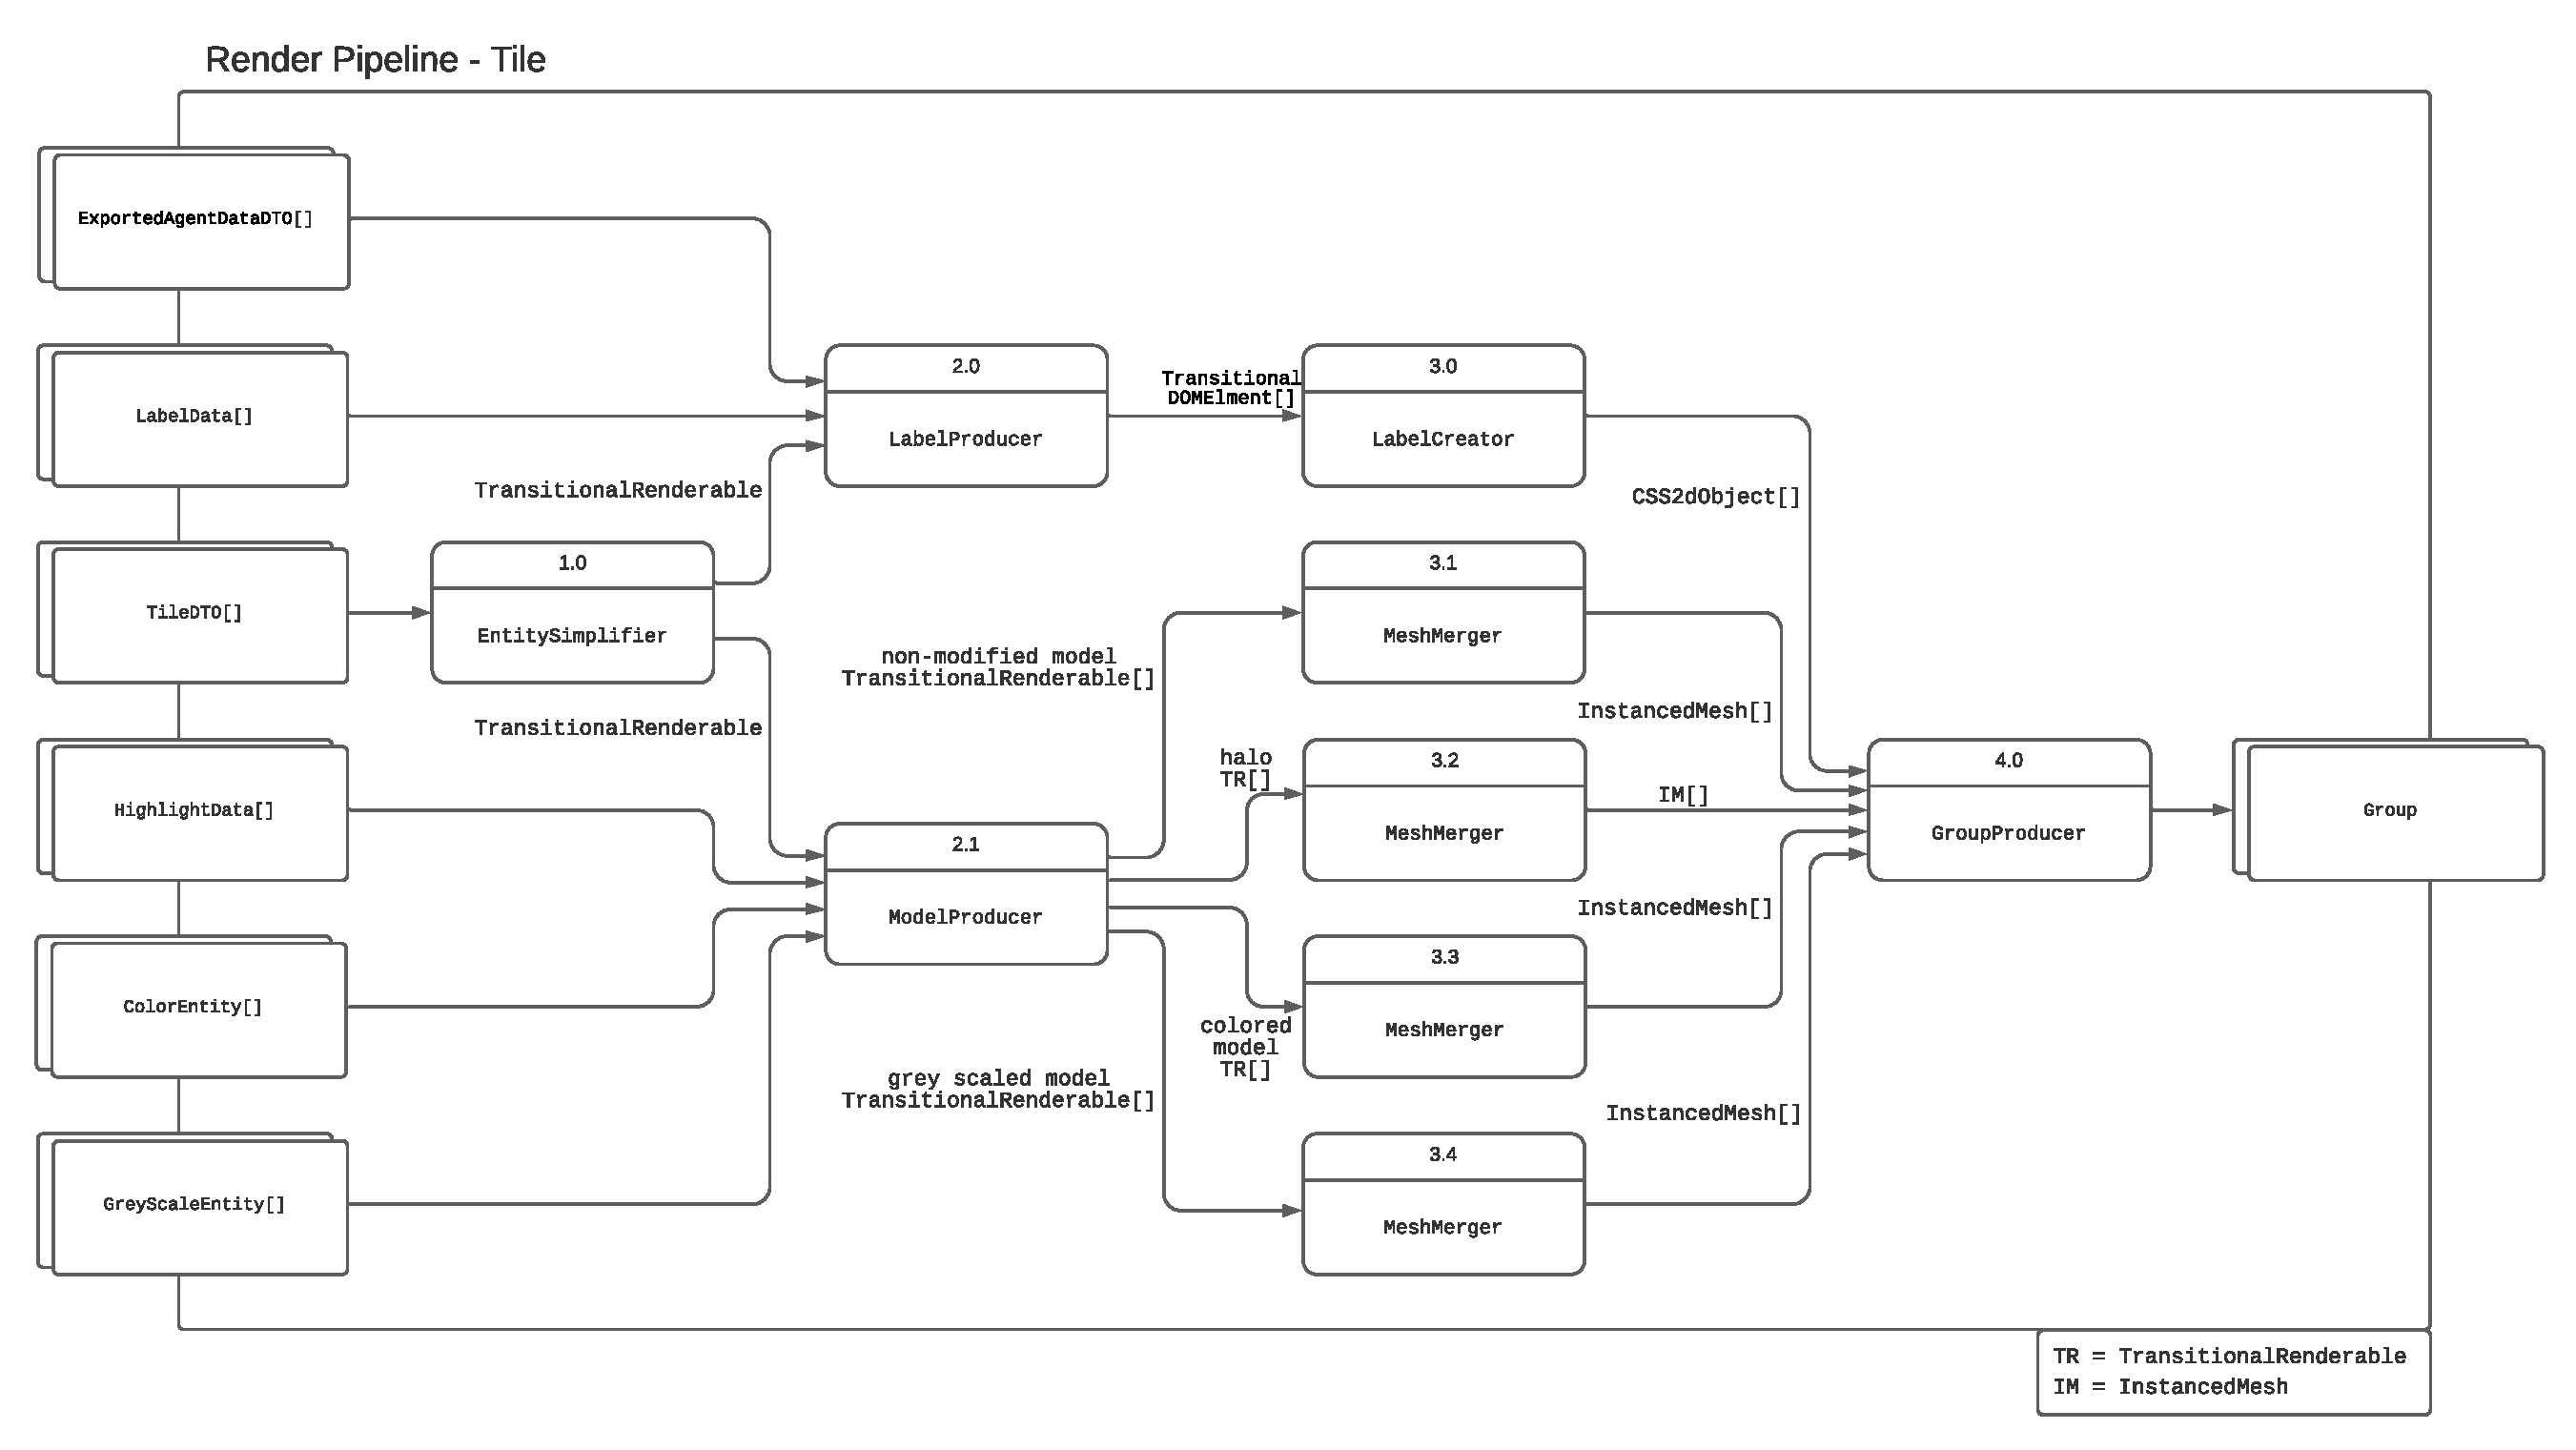
\includegraphics[scale=.65,center]{medien/render-pipeline-dfd.pdf}
    \caption{Render Pipeline: Tile DfD}
    \ownsource
\end{sidewaysfigure}

%\FloatBarrier

Das Diagramm zeigt alle Schritte, die nötig sind, um die Kacheln, die der Handler erzeugt hat bzw. bereitstellt, in solche umzuwandeln, die dem three.js Szenengraph hinzugefügt werden können.
Vom Server bzw. dem Agenten kommen die Entitäten Exported Agent Data DTO und Tile DTO.
Alle weiteren wurden vom Handler auf Grundlage der Nutzerinteraktionen erzeugt.
Beispielweise führt der Klick eines Nutzers zu einer Highlight Data Entität.
Die Grey Scale Entity wird wiederum verwendet, um eine Kachel bei der Platzierung anzudeuten.

Die Datentypen werden im Graphen dann durch den Text an den Kanten angedeutet, dabei wurde aus Lesbarkeitsgründen an einigen Stellen der Datentyp abgekürzt.
Über dem Datentyp wurde, dort wo es nicht eindeutig war, noch der semantische Typ mit angebracht.

Die Umwandlung startet bei der Vereinfachung der Entitäten, wobei aus der Grid Position die eigentlichen Weltkoordinaten errechnet werden.
Aus der Himmelsrichtung-Orientierung wird dann der Quaternion\footnote{\url{https://en.wikipedia.org/wiki/Quaternion}} errechnet.
Diese beiden erzeugen in diesem Schritt auch die 4x4 Matrix, die im weiteren Verlauf für die Positionierung des Modells gebraucht wird.

Besagtes Modell wird ebenfalls in diesem Schritt, durch den beigefügten Tile Type von einem globalen Service angefragt und dem Ausgabewert beigefügt.
Diese Grundlage verwenden dann die Schritte \textit{2.0} und \textit{2.1}.

Schritt \textit{2.0} verwendet dabei die zusätzlichen Eingabedaten, um React mit den entitätstatischen Wrappern und den Agent Data zu versorgen.
Dass der HTML-Wrapper statisch und mit der Entität verknüpft ist, ist wichtig, damit React in der Lage ist, inkrementelle Änderungen anzuwenden und den internen Zustand zu assoziieren, was enorme Ressourcen spart und Interaktivität ermöglicht.

Der Label Producer erzeugt dann ein Ausgabeobjekt, das in einem weiteren Schritt in ein CSS 2D Object umgewandelt wird, das von three.js verwendet werden kann und korrekt in Relation zum Canvas platziert wird.

Schritt \textit{2.1} ist noch einmal bedeutend aufwendiger und sorgt intern dafür, dass alle notwendigen Models und deren Abwandlungen erzeugt werden.
Dafür werden Kopien des Meshes erzeugt und mit neuen Materialien versehen.

Im Anschluss werden all diese Modelle mit ihren Matrizen an die jeweiligen Mesh Merger weiter geleitet.
Hierbei ist es wichtig, dass eine Instanzstabilität herrscht.
Das heißt, dass bei gleicher Eingabe nicht nur die gleiche Ausgabe erzeugt wird, sondern dass auch die Instanzen, die referenziert werden, stabil sind.
So wird bei jeder Tile \textit{34} (eine Gerade), die Grey Scaled werden soll, immer die gleiche 3D-Modell-Referenz zurückgegeben.

Dies und die Aufteilung in mehrere Mesh Merger ist sehr wichtig, damit effizient Instanced Meshes daraus gebildet werden können.
Die jeweiligen Mesh Merger erhalten vollständig getrennte Gruppen von Meshes, die dann intern anhand der Referenz gruppiert werden.
Das Auftrennen in mehrere MeshMerger wirkt wie eine Vorselektierung.
Wenn man sie zusammenführen würde, wäre ihre Laufzeit zwar schlechter, jedoch würde sich an ihrem Verhalten nichts ändern.

Die interne Gruppierung anhand der Modelle wird dann dafür genutzt, um Instanced Meshes\footnote{\url{https://threejs.org/docs/\#api/en/objects/InstancedMesh}} zu erzeugen.
Diese helfen stark dabei, die Darstellungseffizienz zu steigern, indem das eigentliche Modell einmalig (im Hinblick auf die Frames \textbf{und} die Entitäten) an die GPU übertragen wird und im weiteren Verlauf nur noch ein Buffer mit der 4x4 Matrix gefüllt wird, der aktualisiert und pro Frame übertragen werden kann.

Um das ins Verhältnis zu setzten: Das Kachelmodell der Geraden ist 7272 Bytes groß und es handelt sich hierbei um ein einfaches Modell.
Die 4x4 float 32 Matrix ist nur $4*4*32byte=512byte$ groß, somit würden ohne Instanced Meshes $t = n * (7272bytes + 512bytes)$ übertragen werden, wobei n die Anzahl der Geraden repräsentiert.
Mit Instanced Meshes sind es dann nur noch $t = 7272bytes + n * 512bytes$.
Diese Verringerung der Übertragung erlaubt es, mehr Zeit für die eigentliche Darstellung zu nutzen.

Zusätzlich brauchen Operationen wie Mesh-Vereinfachungen nur einmalig angewendet zu werden.
In der Dokumentation von three.js steht diesbezüglich \enquote{Use InstancedMesh if you have to render a large number of objects with the same geometry and material but with different world transformations.}\footnote{\url{https://threejs.org/docs/\#api/en/objects/InstancedMesh}} was genau diesen Fall beschreibt.

In all diesen Schritten werden überall verschiedenste Caches eingesetzt, damit die Referenzstabilität gewährleistet werden kann oder aufwendige Operationen nicht wiederholt werden müssen.

Schlussendlich werden die Ergebnisse in eine Group zusammengefasst und zurückgegeben.

Die hier gezeigten Schritte werden dann noch für Vehicles und Tags wiederholt und dann mit einem abschließenden Schritt zu einer großen Gruppe zusammengefasst, die schlussendlich in den Szenengraphen gehängt wird.

\FloatBarrier


    \subsection{Verteilungssicht}
\label{sec:distribution-view}

Wie bereits im Kapitel \refsec{sec:client-server-arch} beschrieben, soll diese Anwendung als Client Server Anwendung konstruiert werden.
Dabei sind die Artefakte wie in der Abbildung \refimg{fig:client-server-deployment} strukturiert.

\begin{figure}[htb]
    \centering
    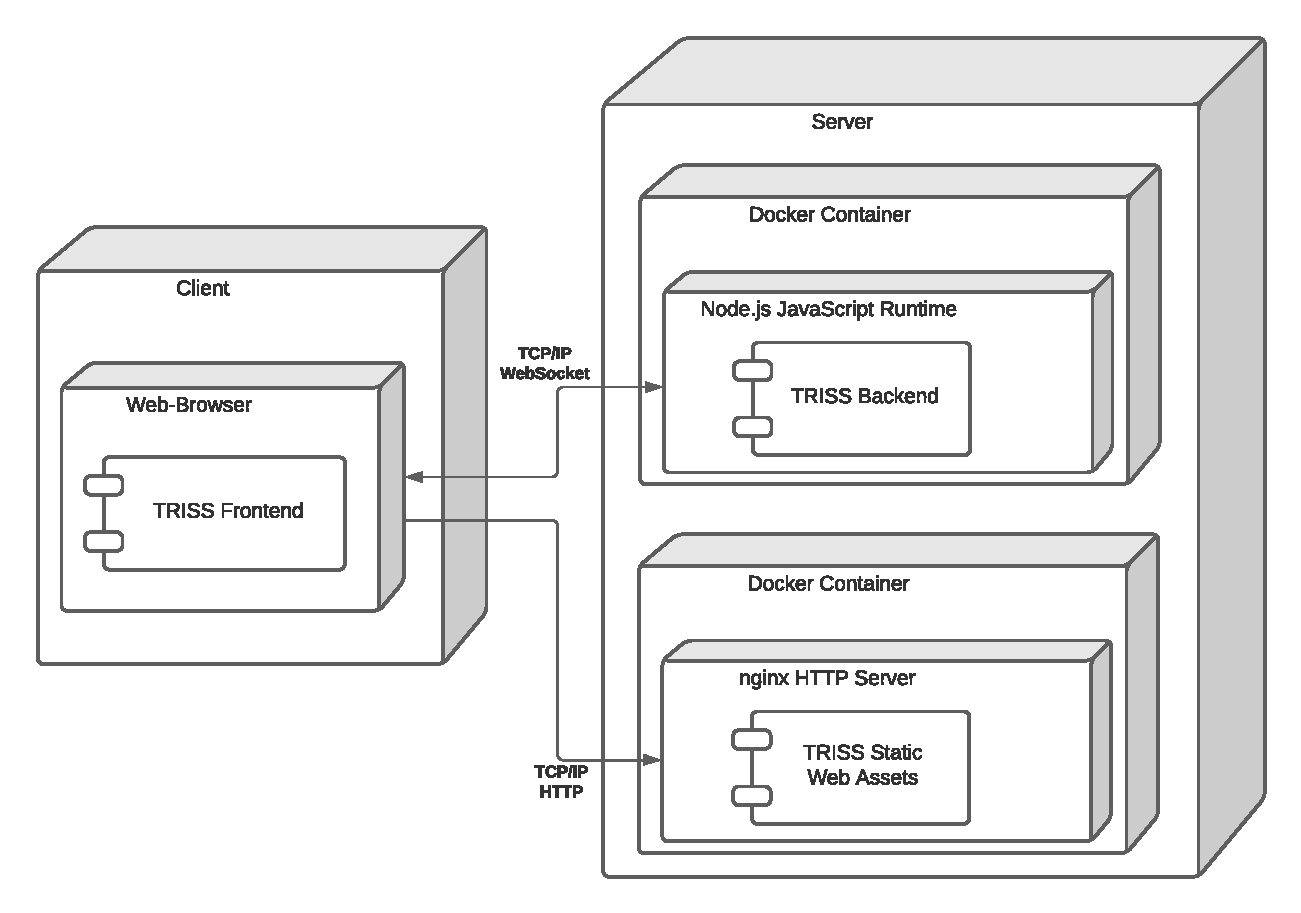
\includegraphics[scale=.65,center]{medien/abstract-client-server.pdf}
    \caption{Client Server Deployment}
    \ownsource
    \label{fig:client-server-deployment}
\end{figure}

\FloatBarrier

Die grundlegende Verteilung zieht dabei bis zu drei physische Systeme in Betracht.
Die drei Systeme würden dann jeweils eine der drei logischen Systeme bzw. deren Laufzeitumgebungen betreiben.

\newcommand{\subsubsubsection}[1]{\paragraph{#1}\mbox{}}

\subsubsection{Artefakt – TRISS Backend}

\subsubsubsection{Rolle}

Das TRISS Backend ist das zentrale System, das den Agenten betreibt sowie die Layouts und den Zustand der Welten verwaltet.

\subsubsubsection{Runtime und äußere Abhängigkeiten}

Bei diesem Artefakt handelt sich um eine JavaScript-Anwendung, die durch eine Node.js v16 Runtime betrieben wird.
Diese Runtime stellt die Standardbibliotheken wie fs, worker\_threads oder http bereit und erlaubt über npm die Verwendung weiterer Bibliotheken.

\subsubsubsection{Erzeugung}

Durch den TypeScript Compiler entsteht eine Sammlung von JavaScript-Dateien, die durch die Einstiegsdateien für den Main Thread und für den Worker eingelesen werden.
Diese werden dann in ein Image verpackt, das als Basis das \textit{node:16}\footnote{\url{https://hub.docker.com/_/node}} Image verwendet.
Als Tag\footnote{\url{https://docs.docker.com/engine/reference/commandline/tag/}} wird \textit{triss-server} genutzt.


\subsubsection{Artefakt – TRISS Frontend}

\subsubsubsection{Rolle}

Das TRISS Frontend hat die gleiche Rolle wie eine typische Webanwendung.
Sie stellt den Server-Zustand dar und erlaubt es dem Nutzer, mit diesem zu interagieren und die Welten zu inspizieren.

\subsubsubsection{Runtime und äußere Abhängigkeiten}

Sie wird durch einen modernen Webbrowser betrieben, der vor allem den Zugriff auf die notwendigen APIs bereitstellt.
So wird hier vor allem auf die OpenGL und die WebSocket API aufgebaut.

\subsubsubsection{Erzeugung}

Das Frontend wird nicht direkt erzeugt, sondern entsteht durch das Beziehen und die darauf folgende Auswertung der index.html.
Diese Komponente repräsentiert hierbei eine konkrete Instanz der Web Assets.
Das Bundle wird, wie auch alle anderen Bestandteile für das Frontend, über HTTP vom Webserver bereits gestellt.

\subsubsection{Artefakt – TRISS Static Web Assets}

\subsubsubsection{Rolle}

Die Static Web Assets repräsentieren die Ressourcen, die für den Betrieb des Frontends benötigt werden.

\subsubsubsection{Runtime und äußere Abhängigkeiten}

Dieses Artefakt wird durch einen nginx Server betrieben bzw. bereitgestellt.
Sein Betrieb benötigt keine weiteren Ressourcen.

\subsubsubsection{Erzeugung}

Gebaut werden die Assets durch Webpack.
Dieses Werkzeug generiert aus den Quelldateien sowie den referenzierten npm-Paketen ein JavaScript-Bundle und erlaubt die Auflösung der Importe innerhalb der Quelldateien.
Zusätzlich beinhalten die Web Assets neben diesem Bundle noch Medien-Dateien, CSS-Spezifikationen und die 3D-Modelle.

Nachdem Webpack dieses Bundle erzeugt hat, wird dieses, ähnlich wie bei dem TRISS Backend Artefakt, durch Docker in ein OCI Image verpackt.
Dabei dient hier das \textit{nginx:1.20}\footnote{\url{https://hub.docker.com/_/nginx}} Image als Basis.

Zusätzlich wird neben den erzeugten Dateien noch die Konfiguration mit in dem Image hinterlegt.

\subsubsection{Deployment}

Es bestehen zwei Wege, um die Anwendung in Betrieb zu nehmen.
Der erste ist, TRISS Backend und TRISS Static Web Assets einzeln aus dem Repository zu beziehen, jeweils zu bauen, die Runtimes zu konfigurieren und zu starten.

Der zweite besteht darin, die beiden Artefakte als OCI Images\footnote{\url{https://opencontainers.org/about/overview/}} zu beziehen und sie dann über eine OCI kompatible Engine zu betreiben.
Dieser zweite Weg ist der vorgesehene, da er einige Vorteile für die Entwicklung und die Inbetriebnahme mit sich bringt.

Ein zentraler Vorteil ist, dass dieses Image, ähnlich zu einer Virtual Machine, self contained ist.
Dieses Image beinhaltet alle Ressourcen, die für die Anwendung gebraucht werden.
Das beginnt bei den Betriebssystem-Schnittstellen und dessen Paketen, zusätzlichen Anwendungen, die installiert sein müssen, über die Runtime, die die Anwendung betreibt, bis hin zu den eigentlichen Dateien, die die Anwendung an sich beinhalten.

Zusätzlich sind sie für die eigentliche Entwicklung vorteilhaft, weil nur die Anforderung zu beachten ist, dass die Anwendung im Kontext eines solchen Containers laufen können muss.
Betrieben wird ein solches Image von einer OCI kompatiblen Engine, diese entkoppelt die Anwendung von dem darunterliegenden Betriebssystem und schirmt sie vollständig voneinander ab, so dass sie sich gegenseitig nicht beeinflussen können.
Somit war es nicht notwendig konkrete Betriebssystem-Versionen auszuwählen, diese zu testen und jeweils Installationsanweisungen zu formulieren.

Im Gegensatz zu einer Virtual Machine ist ein solches Image leichtgewichtiger (benötigt weniger Ressourcen und weniger Speicherplatz) und ist konkret dafür gedacht, eine einzige Anwendung zu kapseln.

Das erlaubt es auch, mit diesem Image anders umzugehen.
So kann dieses mit einem einzigen Kommando aus dem Repository bezogen und dann gestartet werden.
Der Nutzer kann dann beim Start dieses Images noch weitere Konfigurationen vornehmen, wie zum Beispiel Ports umleiten, Geräte freigeben, Hardwarenutzung limitieren, Neustart-Regeln festlegen und Partitionen persistieren.

Für diese Anwendung läuft es also dann darauf hinaus \textit{docker run\linebreak trissapp/triss-server} \textit{docker run trissapp/triss-client} auszuführen.
Näheres dazu im Kapitel \refsec{sec:artefacts}.


    
\subsection{Beispiel Agent – Random Exit Driver}

Der Random Exit Driver (RAD) ist eine Beispiel-Implementation eines Agenten, die im Rahmen dieser Arbeit angefertigt worden ist, um zu demonstrieren, wie man die APIs verwenden kann und wie man dadurch in der Lage ist, Fahrzeuge entlang der Fahrbahnen zu bewegen.

Der Agent ist dafür besonders einfach gehalten, um ihn so gut wie möglich nachvollziehen zu können.
Nicht desto trotz enthält auch er einige aufwendigere Bereiche, die vor allem dabei helfen sollen, ihn auch bei einer größeren Menge von Knoten noch funktional zu halten.

Der eigentliche Umfang ist überschaubar und teilt sich generell in die folgenden zwei Abschnitte.

\subsubsection{Verhaltenslogik}

Der erste ist die eigentliche Logik des Agenten, die in dem Diagramm \refimg{fig:example-agent-sequence} grob umrissen werden soll.

\begin{figure}[htb]
    \centering
    \includegraphics[scale=.65,center]{plant-diagrams/example-agent-sequence.pdf}
    \caption{Ablauf des Beispiel-Agenten}
    \ownsource
    \label{fig:example-agent-sequence}
\end{figure}

\FloatBarrier

Die Schritte \textit{Erzeuge Fahrzeuge} und \textit{Bewege Fahrzeuge} fassen dabei weitere Schritte zusammen.
Sie sind jeweils sehr einfach gehalten.

Der Schritt \textit{Erzeuge Fahrzeuge} läuft im Detail dann folgendermaßen ab.

\begin{figure}[htb]
    \centering
    \includegraphics[scale=.65,center]{plant-diagrams/example-agent-sequence-spawn-vehicles.pdf}
    \caption{Ablauf des Erzeugungsprozesses}
    \ownsource
    \label{fig:example-agent-sequence-spawn-vehicle}
\end{figure}

\FloatBarrier

Begonnen wird damit, alle Spawner-Tags aus der Welt zu filtern.
Diese werden dann im Anschluss sequenziell durchlaufen.
Zu jedem dieser Spawner wurde im Erstellungsschritt des Agenten eine Tabelle mit allen verfügbaren Routen hinterlegt.
Diese wurden dann nach den anliegenden Kacheln, also der ersten Kachel der Route, gruppiert.

Diese Gruppen werden dann durchlaufen und aus jeder wird dann eine zufällige Route verwendet, daher auch der Name, Random Exit Driver.
Unabhängig davon, welche Route gewählt wurde, ist die erste Kachel all dieser Routen die gleiche, damit hätte auch die darauf folgende Kollisionsprüfung das gleiche Ergebnis.

Sollte der Platz noch frei sein, platziert der Agent eine zufällige Fahrzeugklasse und hinterlegt im Agenten, welches Modell sich auf welcher Route mit welchem Ziel befindet.
Dieser Eintrag ist dann der eigentliche Kenntnisstand des Agenten, Fahrzeuge in der Welt ohne diesen Eintrag werden nicht behandelt.

Der Schritt \textit{Bewege Fahrzeuge} baut darauf auf und verwendet vor allem diesen Eintrag im Register.

\begin{figure}[htb]
    \centering
    \includegraphics[scale=.65,center]{plant-diagrams/example-agent-sequence-move-vehicles.pdf}
    \caption{Ablauf des Bewegungsprozesses}
    \ownsource
    \label{fig:example-agent-sequence-move-vehicle}
\end{figure}

\FloatBarrier

Es wird nun sequenziell durch alle Fahrzeuge iteriert und für jedes der Registereintrag geladen.
Der Grund, warum dieser getrennt gespeichert und nicht an dem Fahrzeug Objekt angeheftet wird, ist, dass dem Agenten nicht garantiert wird, dass es noch die gleiche Objektinstanz ist.

Sollte die aktuelle Distanz auf der Route der maximalen Länge der Route entsprechen, wird das Fahrzeug aus der Welt und dem Register entfernt, wenn nicht, wird eine statische Distanz auf die aktuelle Distanz addiert (es wird keine Beschleunigung simuliert) und dann geprüft, ob bei der neuen Position eine Kollision entsteht.

Falls das nicht der Fall sein wird, wird das Fahrzeug an diese Position verschoben.
Die Kollisionsinformation, die für diese Abfrage verwendet wird, wird allerdings nicht direkt aktualisiert.

Das erlaubt es dem Agenten, diesen Abschnitt auf mehrere Realms zu verteilen und die Verschiebung parallel zu errechnen.
Auch wenn dies hier noch nicht genutzt wird, eliminiert es zusätzlich Probleme, die durch eine unterschiedliche Behandlungsreihenfolge entstehen würden.

Schlussendlich wird die Kollisions-Tabelle kumulativ aktualisiert.

\subsubsection{Hilfsstrukturen}

Das oben aufgeführte Verhalten ist so in zwei bzw. drei Methoden in der Agenten-Klasse implementiert.
Jedoch hatte sich bei der Entwicklung und Implementierung gezeigt, dass die hohen Laufzeitkomplexitäten die eigentliche Nutzbarkeit stark beschränken.

So muss bei jeder Bewegung des Fahrzeuges, bei einer naiven Implementation, zu jedem anderen Fahrzeug geprüft werden, ob es kollidieren würde.
Somit besteht hier eine Komplexität von $O(n^2)$.
Bei der Erzeugung der Fahrzeuge besteht das gleiche Problem und zusätzlich wird dies durch die Anzahl der Spawner multipliziert.
Dazu kommt noch die Routenfindung, die bei der naiven Implementation auch bei jedem Frame erneut durchgeführt werden müsste.

Bei dieser Routenfindung wird dann von jedem Spawner zu jedem anderen Spawner versucht, eine Route zu finden, wobei diese jeweils dann als Breitensuche über die Kacheln implementiert ist, welche ebenfalls eine Laufzeit von $O(n^2)$ hat.

In der Realität zeigt sich, dass selbst Szenarien mit vier Spawnern und 30 Kacheln bereits eine hohe Auslastung erzeugen.

Um dem entgegenzuwirken, wurden Caches erstellt, die einfache Ausschlusskriterien verwirklichen und Ergebnisse vorberechnen.
Diese Caches selbst wurden sehr einfach gehalten und sind nur als Beispiele zur Beschleunigung zu verstehen.

Der erste Cache ist der Navigator, der direkt zu Beginn alle möglichen Routen errechnet und diese dann anhand der ersten Kachel gruppiert.
Dieser Cache wird vom Spawner verwendet und braucht nicht aktualisiert zu werden, da dieser Beispiel-Agent keine Veränderungen an den Kacheln vornimmt.

Der Collision-Cache ist der, der von der Bewegungsroutine verwendet wird, um zu überprüfen, ob ein Fahrzeug mit einem anderen kollidiert.
Er verwendet intern ein Zellensystem, das Fahrzeuge all den Zellen zuordnet, in denen sich Teile seiner Geometrie befinden.
Dadurch wird in der Verwendung die eigentliche Menge an Kollisionsberechnungen drastisch reduziert.

Zusätzlich speichert dieser Cache auch ab, was das Ergebnis einer Kollision zwischen den Fahrzeugen \textit{A} und \textit{B} war, und gibt dieses Resultat bei allen erneuten Anfragen zwischen diesen beiden Parametern und auch der Abfrage zwischen \textit{B} und \textit{A} wieder.

Dieser Cache wird im Verlaufe der Simulation ständig aktualisiert, wobei dann der Cache für die Abfrage, bei der \textit{A} beteiligt ist, verworfen wird und die Zellenzuordnung erneut berechnet wird.

Beide Caches erlauben eine Verwendung des Agenten mit einer bedeutend größeren Menge an Fahrzeugen, limitieren jedoch nicht die logische Erweiterung des Verhaltens, sodass Beispielweise die Beachtung von rechts vor links ohne Anpassung dieser möglich wäre.


% 1325 lines 10 files



    \section{Resultatbetrachtung} \label{sec:reflection-main}

Nach der Fertigstellung dieser Anwendung musste diese noch auf ihre Eignung geprüft werden.
Dafür sollten, neben der funktionalen Prüfung, zwei Dinge sichergestellt werden.

Zum einen soll gezeigt werden, wie einfach es ist, Agenten zu implementieren, und welche limitierenden Faktoren dabei auftreten.
Zum anderen soll gemessen werden, welche eigentliche Performance diese Anwendung auf weißt, da diese, wie in Qualitätsziel \textit{QLT\#01} und \textit{QLT\#02} beschrieben, für die eigentliche Verwendung eine große Rolle spielt.


    
\subsection{Einfachheit der Agentenentwicklung}

Ein relevantes Resultat ist, welche Einschränkung diese Anwendung für die Entwicklung des Agenten vorgibt: je nachdem würde das erlauben, bestimmte Arten von Agenten gar nicht erst zu entwickeln oder zu betreiben.
Dies kann sich auch stark auf die Einstiegshürde auswirken.

Das eigentliche Interface, das ein Agent erfüllen muss, ist sehr einfach gehalten.
Es beschränkt sich auf zwei zu implementierende Methoden, wobei \textit{getExportedAgentData} optional ist, insofern es dem Entwickler helfen soll, das Verhalten seines Agenten zu untersuchen.

Die Methode \textit{handleFrame} ist die einzige erforderliche.
Bei ihrem Aufruf werden die \textit{World}, die aktuellen Frame-Nummer und die Frame-Zeiten übergeben und eine World als Antwort erwartet.
Wie genau der Agent diese also erzeugt ist nicht vorgegeben oder eingeschränkt.

Dabei kann dieser Fahrzeuge erzeugen oder entfernen, von einen Ort an einen anderen teleportieren oder sich um seine Achse drehen lassen.
Die eigentliche Veränderung wird nicht überprüft und das aktuelle Layout nicht in Betracht gezogen.
Letzteres kann der Agent durch die Welt nicht nur abtasten, sondern auch verändern.

Für die Verarbeitung stellt der Server Funktionen bereit, um beispielweise die Spuren zu ermitteln, diesen zu folgen oder Distanzen auf einer Strecke zu errechnen.
Zusätzlich dazu implementiert der Random Exit Driver eine Kollisionsberechnung, die für einen neuen Agenten verwendet werden oder als Grundlage für eine andere Implementation dienen kann.

Einschränkend wirkt nur, dass der Agent diskrete Zustände erzeugen muss.
Insofern ist eine sehr offene API geschaffen worden, die die unterschiedlichsten Entwicklungen unterstützen sollte.

Die Sprache JavaScript und das Ökosystem erlauben hier zusätzlich viele Freiheiten.
Das liegt nicht zuletzt daran, dass die Sprache sehr einsteigerfreundlich ist, keine explizite Speicherverwaltung erfordert, keine Parallelität besitzt und viele Programmierparadigmen unterstützt, sondern auch daran, dass das Ökosystem durch npm viele unterschiedliche sehr aktuelle Pakete bereitstellt.
So können via npm sogar beispielweise die Entwicklung und Nutzung von neuronalen Netzen ermöglicht bzw. beschleunigt werden\autocite{tensorflowTut2022}.

Selbst dann wenn die Schnittstelle oder Bibliothek noch nicht als npm Paket verfügbar ist, kann man diese trotzdem via WebAssembly oder Nativen Add-ons nutzen.


    \subsection{Effizienz der Anwendung} \label{sec:application_efficiency}

Für die Überprüfung der Effizienz wurden der Server und der Client auf dem gleichen System betrieben.
Dabei wurde eine leere Welt mit einem Agenten kombiniert, der Fahrzeuge nach einem festen Muster bewegt.

Dieser Agent soll ganz gezielt so wenig wie möglich Zeit benötigen, da der Fokus hier auf den restlichen Komponenten liegt.

Die Messung wurde mit dem Chrome Browser Version 100.0.4896.75 und der Node.js Runtime Version v16.13.1 durchgeführt.
Die Anwendung wurde auf einem Computer mit einer Nvidia GForce 1060 3 GB, einem AMD FX 8320 8-Kern Prozessor und 32 GB RAM betrieben.
Als Betriebssystem diente Windows 10 Version 19044.

Der Agent wurde nun gestartet und für 10 Sekunden betrieben, dabei bewegt dieser abhängig vom aktuellen Frame die Fahrzeuge in einem Wellenmuster.
Vier Komponenten wurden dann gezielt mit Messpunkten versehen.
Diese Komponenten sind die, deren Laufzeit von der Anzahl der Fahrzeuge abhängt.

Diese Komponenten stellen die zentrale Abfolge aus \textit{Rendering} (dem Render-Pipeline- und three.js-Schritt), \textit{Deserializing} (die Frontend seitige Umwandlung von Binärdaten in JavaScript-Objekte), \textit{Serializing} (die Umwandlung von JavaScript-Objekten zu einer Binärrepräsentation im Worker) und schließlich dem \textit{Step} (die Erzeugung eines neuen Frames durch den Agenten) dar, die für jeden Frame durchlaufen werden muss.

\begin{table}[h!]
    \footnotesize{
        \makebox[\textwidth][c]{
            \begin{tabular}{ |r|r|r|r|r|r|r|r|r|  }
                \hline
                \multirow[b]{3}{4em}{Fahrzeuge} & \multicolumn{4}{c|}{Client Realm} & \multicolumn{4}{c|}{Agent Worker Realm} \\
                \cline{2-9}
                & \multicolumn{2}{c|}{Rendering} & \multicolumn{2}{c|}{Deserializing} & \multicolumn{2}{c|}{Serializing} & \multicolumn{2}{c|}{Step} \\
                \cline{2-9}
                & Time    & Rate       & Time    & Rate       & Time    & Rate       & Time   & Rate        \\
                \hline
                256    & 0,63ms  & 1.585,20Hz & 0,21ms  & 4.660,19Hz & 0,47ms  & 2.150,11Hz & 0,03ms & 29.408,88Hz \\ % real 53 hz im frontend, 56Hz im Backend
                512    & 0,75ms  & 1.325,23Hz & 0,39ms  & 2.561,37Hz & 0,82ms  & 1.215,89Hz & 0,04ms & 25.365,15Hz \\ % 52 real, 56 Backend
                1.024  & 0,99ms  & 1.010,10Hz & 0,79ms  & 1.273,21Hz & 1,19ms  & 840,96Hz   & 0,05ms & 20.244,45Hz \\ % 51 real, 56 Backend
                2.048  & 1,38ms  & 726,39Hz   & 1,47ms  & 678,16Hz   & 2,47ms  & 404,14Hz   & 0,21ms & 4.671,12Hz  \\
                4.096  & 2,86ms  & 349,96Hz   & 3,43ms  & 291,16Hz   & 4,56ms  & 219,22Hz   & 0,48ms & 2.103,71Hz  \\ % real 48, 54
                8.192  & 7,97ms  & 125,54Hz   & 9,46ms  & 105,68Hz   & 10,19ms & 98,16Hz    & 0,70ms & 1.435,29Hz  \\ % 36, 50
                16.384 & 14,27ms & 70,09Hz    & 20,51ms & 48,76Hz    & 27,20ms & 36,76Hz    & 0,73ms & 1.377,13Hz  \\ % 20, 28
                32.768 & 31,60ms & 31,65Hz    & 41,25ms & 24,24Hz    & 40,77ms & 24,53Hz    & 1,31ms & 766,04Hz    \\ % 10, 17
                \hline
            \end{tabular}
        }
    }
    \caption{Verarbeitungsgeschwindigkeitsmessung}
    \ownsource
    \label{table:2}
\end{table}

\textit{Time} ist die Zeit für einen Durchlauf der Komponente mit der jeweiligen Menge an Fahrzeugen und \textit{Rate} drückt dann das Inverse, also die mögliche Anzahl an Durchläufen pro Sekunde, aus.

Wie zu erkennen ist, beschränkt im stärksten Maße die (De-)Serialisierung.
Diese benötigt bei 32.768 Fahrzeugen auf beiden Seiten rund 40 ms womit die eigentlich Framerate sowohl bei der Erzeugung als auch bei der Darstellung auf 25Hz beschränkt ist.

Ein zusätzlicher Faktor sind die Datenmengen, die transportiert und dann im Speicher abgelegt werden müssen.
Bei 32.768 Fahrzeugen erreicht der Frame ein Volumen von 1.015.844 Bytes, die durch die Serialisierung erzeugt werden.
Das heißt bei 60 Hz müssten 60,95 MB pro Sekunde übertragen werden, womit mindestens eine Übertragungsrate von 488 MBit pro Sekunde benötigt werden würde.

Diese Datenraten erreicht man nur noch in ausreichend ausgestatteten lokalen Netzwerken, die eine Übertragungsrate von 500 MBit bzw. einem Gigabit zulassen.
Jedoch handelt es sich hierbei schon um eine sehr große Menge an Fahrzeugen.

Bei 4096 Fahrzeugen, was eine realitätsnähere Obergrenze sein sollte, sind das dann nur noch 61 Mbit pro Sekunde und bei 1024 Fahrzeugen 15 Mbit pro Sekunde.
Durch 1024 Fahrzeugen sollten schon viele Szenarien abdecken und einen großen Anteil an Wechselwirkungen erkennen lassen.
Durch die dafür benötigten 15 Mbit Up- bzw. Download ließen sich diese Simulationen dann sowohl über das Internet als auch im lokalen Netzwerk übertragen.

Größere Datenmengen erzeugen allerdings auch Probleme durch ihre Deserialisierung.

Bei 32.768 Fahrzeugen erhöht sich innerhalb 600 ms der allokierte Speicher im Browser, größtenteils durch die Deserialisierung, von 30 MB auf mehr als 130 MB, was dann eine Garbage Collection nach sich zieht.
Dadurch, dass diese den JS Thread blockiert, verringert sich der Anteil der Gesamtzeit, die das Script mit der Berechnung verbringt, auf nur noch etwa drei Viertel der real vergangenen Zeit.

\begin{figure}[htb]
    \centering
    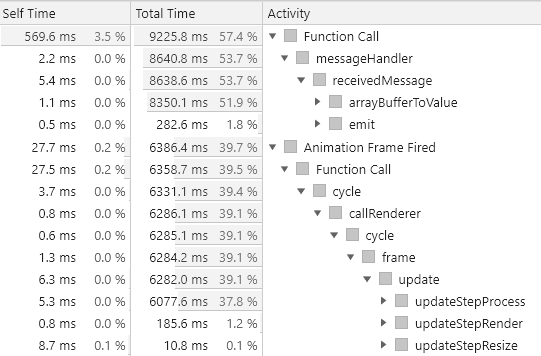
\includegraphics[scale=0.5,center]{medien/triss-perf.png}
    \caption{TRISS Performance Measurements}
    \ownsource
    \label{fig:triss-performance}
\end{figure}

Die eigentliche Pipeline nutzt von der gesamten JavaScript-Zeit etwa 37 \% (28 \% der realen Zeit), der eigentliche Pixel-Erzeugungsprozess durch WebGL ist nicht erfassbar.
Der Deserialize-Schritt braucht in etwa 52 \% (39 \% der realen Zeit) dieser Zeit.

In jedem Fall steht, vor allem im Bereich unter 4096 Fahrzeugen, serverseitig mit 70 \% der Zeit noch ein bedeutender Anteil der Rechenleistung für den Agenten bereit und das selbst dann, wenn man bei diesem einen Worker bleibt.
Die Implementation des Agenten könnte ebenso gut auf mehrere Worker verteilt werden, wodurch dann die restlichen Kerne ausgelastet werden könnten.
Mit 4096 Fahrzeugen sollten sich allerdings schon sehr viele unterschiedliche Szenarien abdecken und simulieren lassen.

Somit wirkt diese Implementation mit dem JavaScript-Ökosystem nicht als \enquote{Flaschenhals} und steht damit selbst bei aufwendigeren Szenarien dem Agenten nicht im Weg.


    \subsection{Erfüllung der funktionalen Anforderungen}

Wie zu erkennen ist, ließen sich die nicht funktionalen Anforderungen ausreichend erfüllen.
Im Folgenden soll nun überprüft werden, ob dies auch auf die funktionalen Anforderungen zutrifft.

Dafür sollen diese hier aufgelistet und dann einzeln auf diese eingegangen werden.
Dabei soll durch Screenshots die tatsächliche Realisierung angedeutet werden.

\subsubsection{FNC\#01 – Definition eines Straßenlayouts}

Die Implementation der Anforderung \refgoal{fnc:define_layout} ist vor allem im Datenmodell zu erkennen, insofern durch dieses das eigentliche Raster repräsentiert worden ist.
Um diese Anforderung zu erfüllen, wurden verschiedenste Kachel-Modelle erworben und mit den jeweiligen Spur Informationen versehen.

Durch das gleichmäßige Raster können, wie vorgesehen, sowohl Agenten als auch Nutzer mit ihm leicht umgehen.
Ein Beispiel dafür, wie ein Agent dieses Raster nutzen kann, ist im vorgefertigten Random Exit Driver beigelegt.
Dieser nutzt das Kachelmodell, um dadurch effiziente Caches für die Wegfindung aufzubauen.
Die zeitlich praktikable Implementation dieses Caches funktionierte hier primär durch diese Limitierung.

Für den Nutzer ist diese Art des Modells ebenfalls einfacher, da das Raster leichter nachzuvollziehen und zugänglicher ist als eine Freiform-Positionierung.
Zusätzlich muss hierfür der Nutzer nicht so geschickt sein und macht dadurch weniger Fehler bei der Definition.
Dies ist auch in der Ausführung für die Anforderung \refsec{sec:check-fnc-3} zu erkennen.

Für die Erstellung eines solchen Layouts wird der Nutzer anfangs vor die Wahl gestellt, ob er ein anderes Layout als Grundlage verwenden möchte.
Er kann dabei aus bereits existierenden Layouts wählen und diese dadurch erweitern bzw. nach Belieben anpassen.
Sollte er das nicht wollen, kann er, wie in Abbildung \refimg{fig:layout-base} zu erkennen, auch mit einem leeren Layout fortfahren.

\begin{figure}[htb]
    \centering
    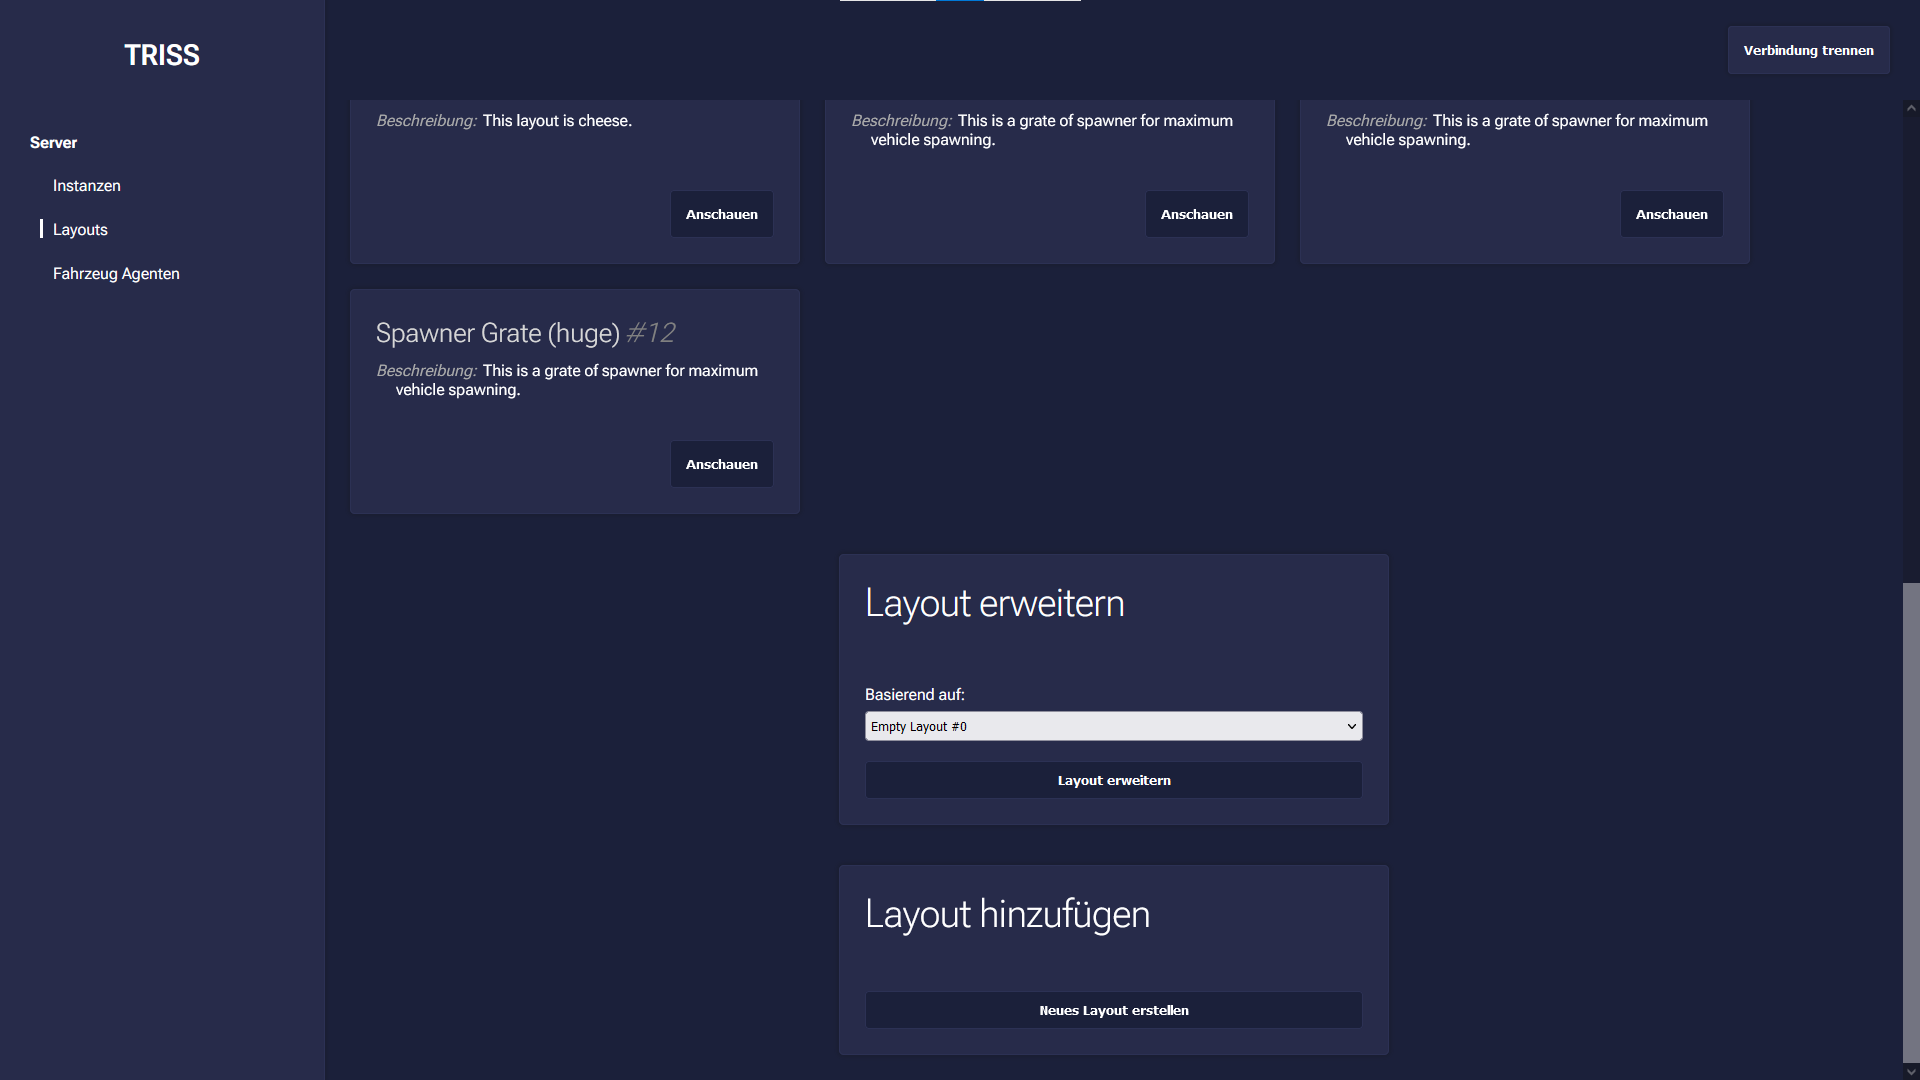
\includegraphics[scale=.25,center]{medien/screenshots/layout-base.png}
    \caption{Layout Grundlage auswählen}
    \ownsource
    \label{fig:layout-base}
\end{figure}

Nach dem Auswählen ist er in der Lage, die Metainformationen zu hinterlegen und, wie in \refgoal{fnc:configure_layout} beschrieben, Kacheln zu platzieren.

\FloatBarrier

\subsubsection{FNC\#02 – Inspektion eines Straßenlayouts}

Diese Anforderung ließ sich mithilfe der bereits genannten Modelle sowie mit der three.js Bibliothek voll umsetzen.
Alle auf dem Server gespeicherten Layouts werden für den Nutzer in einer Liste, wie in \refimg{fig:choose-layout} abgebildet, dargestellt.
In dieser Liste wird für jede Entität der Name, die Identifikationsnummer sowie die Beschreibung angezeigt.

\begin{figure}[htb]
    \centering
    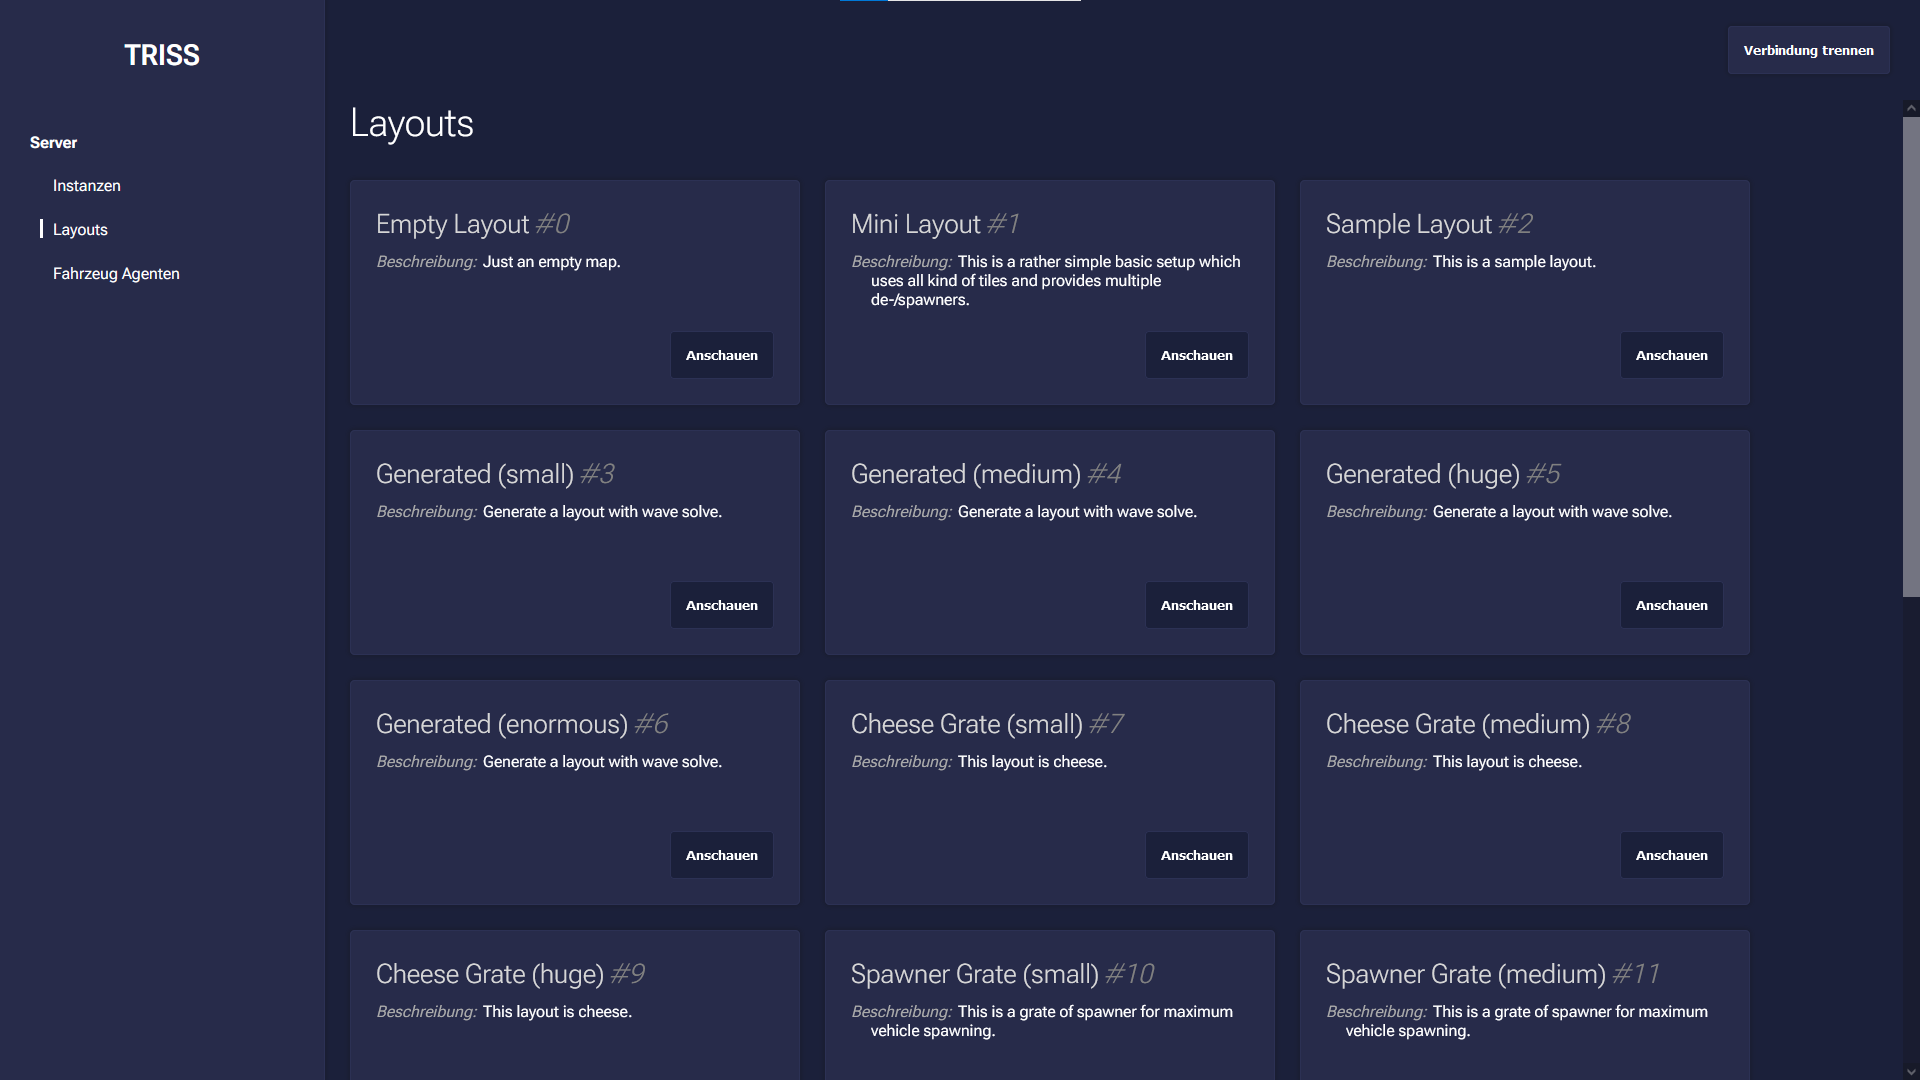
\includegraphics[scale=.25,center]{medien/screenshots/choose-layout.png}
    \caption{Layout auswählen}
    \ownsource
    \label{fig:choose-layout}
\end{figure}

Durch das Drücken auf \textit{Anschauen} wird das Layout für das Betrachten ausgewählt.
Damit dieses dargestellt werden kann, wird dieses zuerst vom Server bezogen und im Anschluss an die Komponente für die Darstellung weitergereicht um dann die Darstellung, wie in \refimg{fig:layout-view} zu sehen, zu erzeugen.

\begin{figure}[htb]
    \centering
    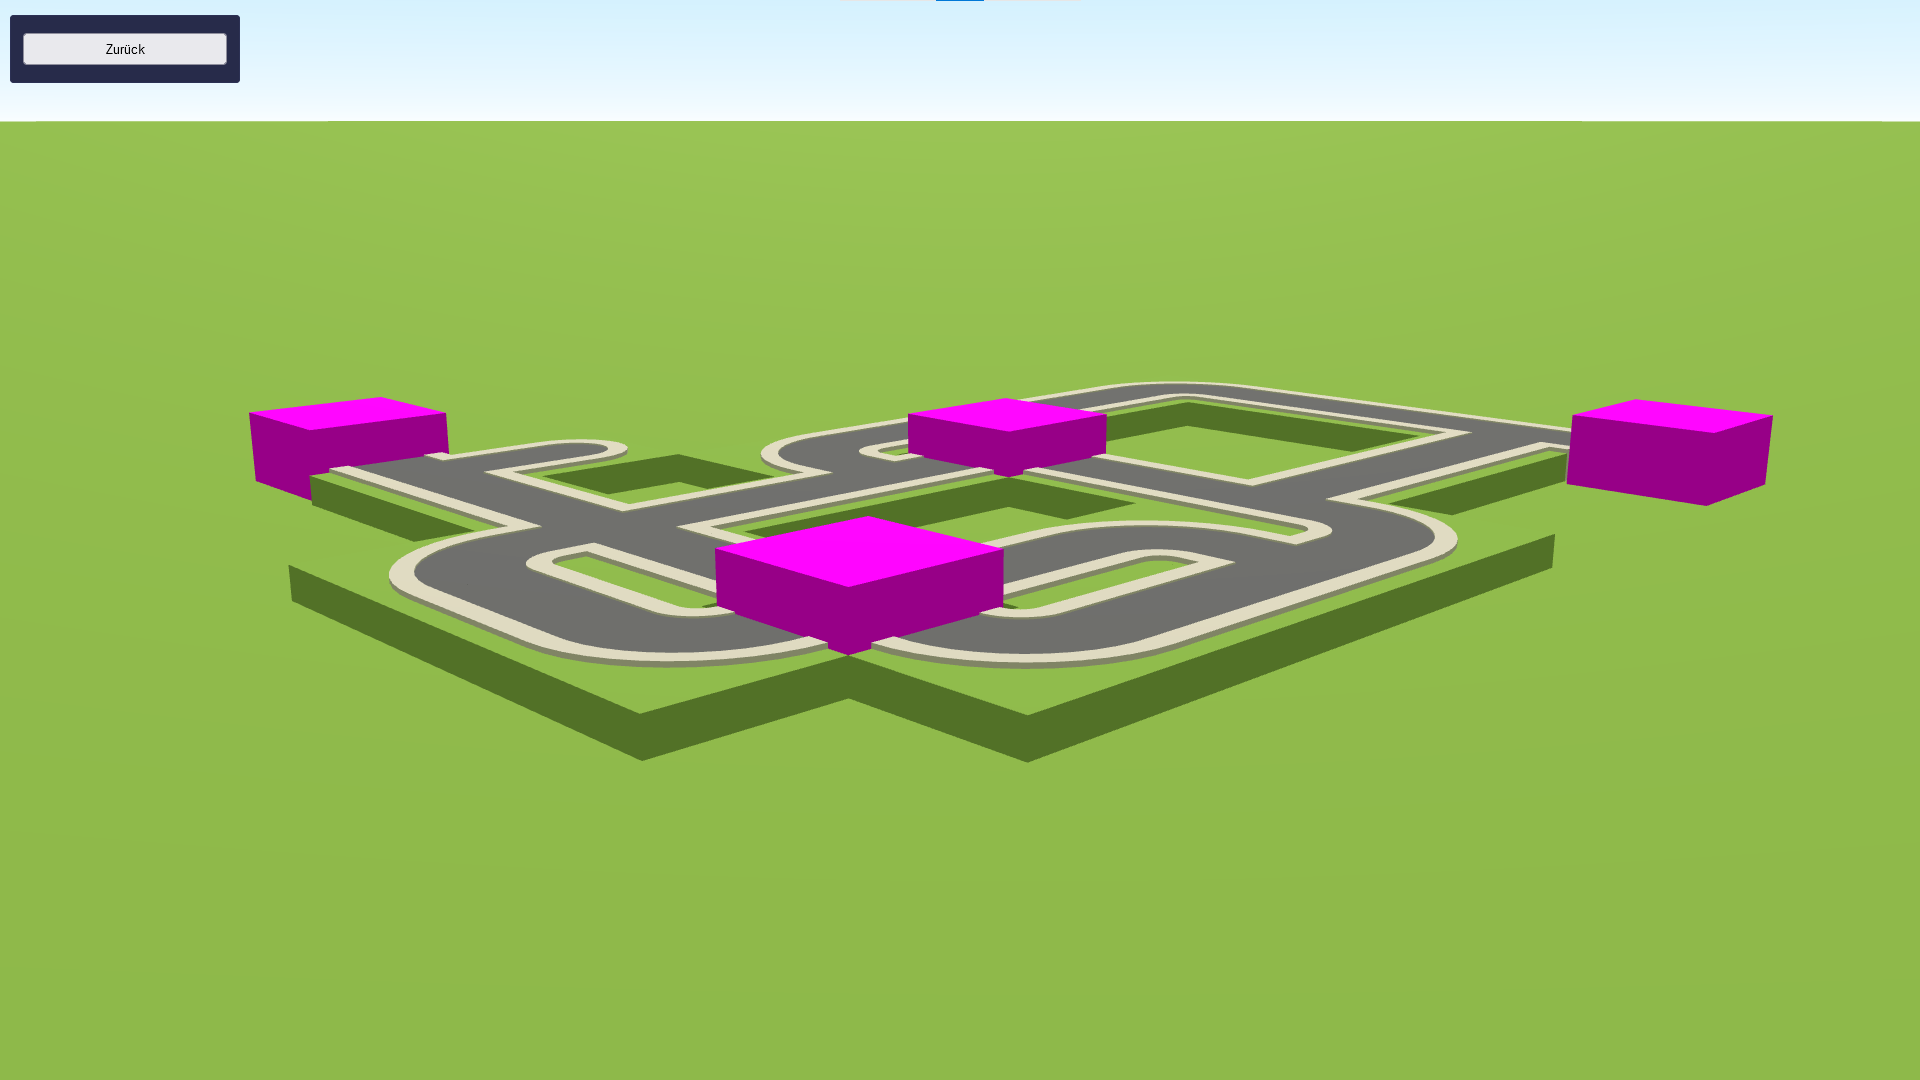
\includegraphics[scale=.25,center]{medien/screenshots/layout-view.png}
    \caption{Layout inspizieren}
    \ownsource
    \label{fig:layout-view}
\end{figure}

In dieser kann man dann via der Maus die Ansicht rotieren und mit dem Mausrad die Kamera herein- und herausbewegen.
Somit lässt sich das Layout frei inspizieren und nachvollziehen.

%\FloatBarrier

\subsubsection{FNC\#03 – Platzierung einer Kachel} \label{sec:check-fnc-3}

Für das Platzieren der Kachel wurde eine ähnliche Ansicht erstellt wie die, die für die Anforderung \refgoal{fnc:inspect_layout} verwendet worden ist.

So kann der Nutzer auch hier mit der Maus die Kamera frei bewegen.
Zusätzlich erhält er weitere UI-Elemente, wie in \refimg{fig:place-ui} abgebildet, durch die er in der Lage ist, Kacheln zu platzieren.

\begin{figure}[htb]
    \centering
    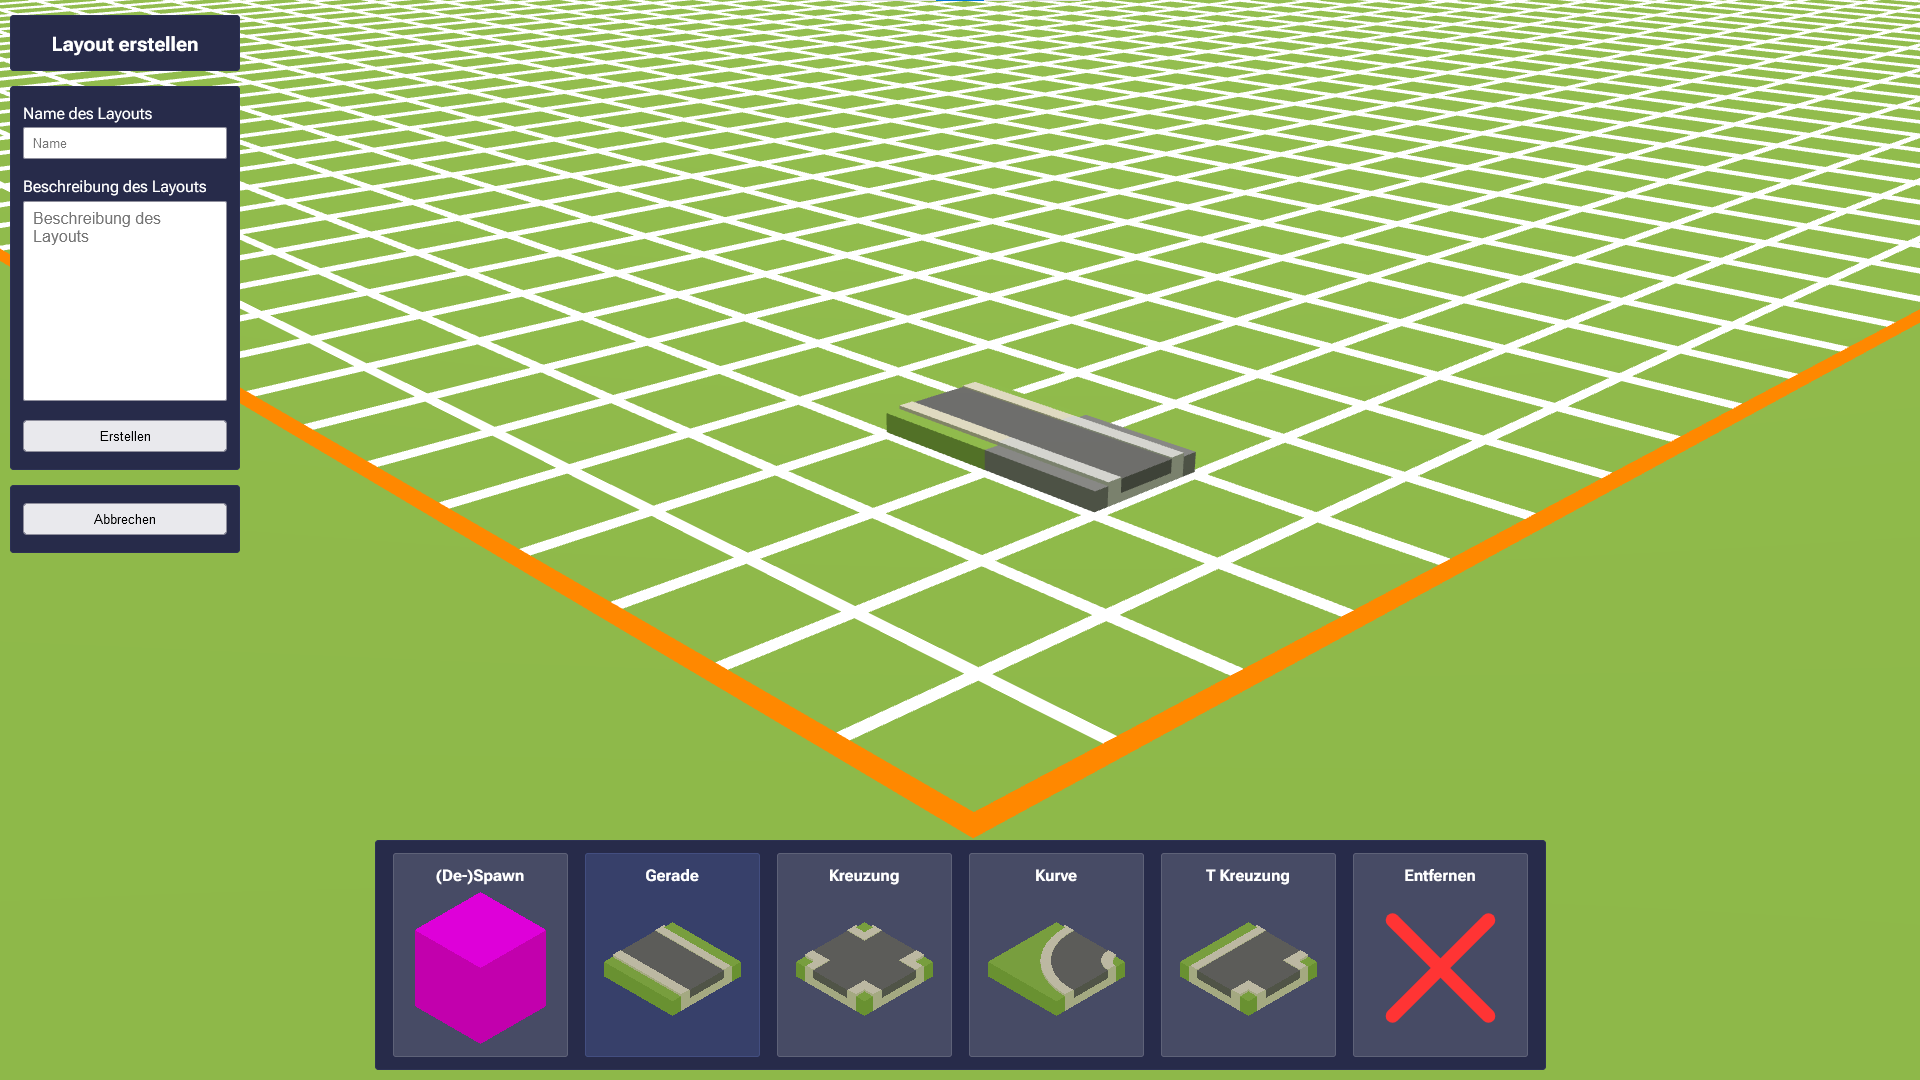
\includegraphics[scale=.25,center]{medien/screenshots/place-ui.png}
    \caption{UI für die Erstellung eines Layouts}
    \ownsource
    \label{fig:place-ui}
\end{figure}

Dabei kann der Nutzer über die Elemente auf der linken Seite die Metadaten für das Layout spezifizieren und mit der Auswahlliste in der unteren Hälfte festlegen, welche Wirkung der Linksklick aktuell hat.

Bei allen Optionen, bis auf die \textit{Entfernen} Funktion, hat der Nutzer beim Bewegen der Maus über das Raster eine schattierte Version der ausgewählten Kachel, die dem Cursor folgt.
Wenn man dann via Linksklick die Kachel platziert, nimmt diese ihre korrekte Farbe/Textur an und verbleibt an dem Ort, an dem sie vorher dargestellt worden ist.

So lassen sich Kacheln auch überschreiben und via den Tasten \enquote{,} und \enquote{.} rotieren.
Durch die letzte Option kann der entfernen Modus aktiviert werden, wodurch bei einem Linksklick die Kachel wieder entfernt wird.

Diese Implementation sollte die komplette Anforderung erfüllen, auch wenn hier nicht alle Kacheln für das Platzieren zur Verfügung gestellt werden.

%\FloatBarrier

\subsubsection{FNC\#04 – Spezifikation eines Agenten}

Die Spezifikation ist aufwendiger zu implementieren gewesen und hat sich im Verlauf der Entwicklung auch zwei Mal grundsätzlich verändert.

Bei der finalen Implementation ist statt den Metafeldern nur noch der Upload vorhanden.
Dieser erwartet nun im Wurzelverzeichnis eine \textit{package.json}, die den Namen und die Beschreibung beinhaltet und dann aus dieser heraus gelesen wird.
Dies soll eine Dopplung von Informationen verhindern und damit Änderungsanomalien vorbeugen.

Die Dateien werden dann in den Workspace geschrieben und via Yarn installiert, das heißt, dass diese nun korrekt externe Abhängigkeiten haben können und damit dem Agenten noch mehr Freiheiten geben, wie dieser intern funktioniert.

Die restliche Spezifikation ist, wie in dem vorangegangenem Evaluationskapitel zu erkennen, so wenig einschränkend wie möglich.

\subsubsection{FNC\#05 – Betrieb einer Simulation}

Diese Anforderung konnte ziemlich genau so implementiert werden, wie es vorgesehen war.
Vor allem auf den Aspekt der Isolation konnte hier eingegangen werden, indem mit Workern ein eigener Kontext geschaffen worden ist und dadurch, selbst wenn dieser viele externe Bibliotheken benötigt, diese nicht direkt für alle geladen werden.

\subsubsection{FNC\#06 – Inspektion einer Simulation}

Die Umsetzung dieser Anforderung war die aufwendigste und vielseitigste.
Das lag vor allem daran, dass sie zusammen mit der nicht funktionalen Anforderung \refgoal{qlt:rendering_efficiency} mehrere Gesichtspunkte hatte, die im Zusammenspiel eine sehr solide Implementation erforderten, um sie zu erfüllen.
Dies ist allerdings, wie auch bereits in dem Abschnitt \refsec{sec:application_efficiency} beschrieben, sowohl im Hinblick auf die Leistungs- als auch auf die Funktionalen-Merkmalen gelungen.

\begin{figure}[htb]
    \centering
    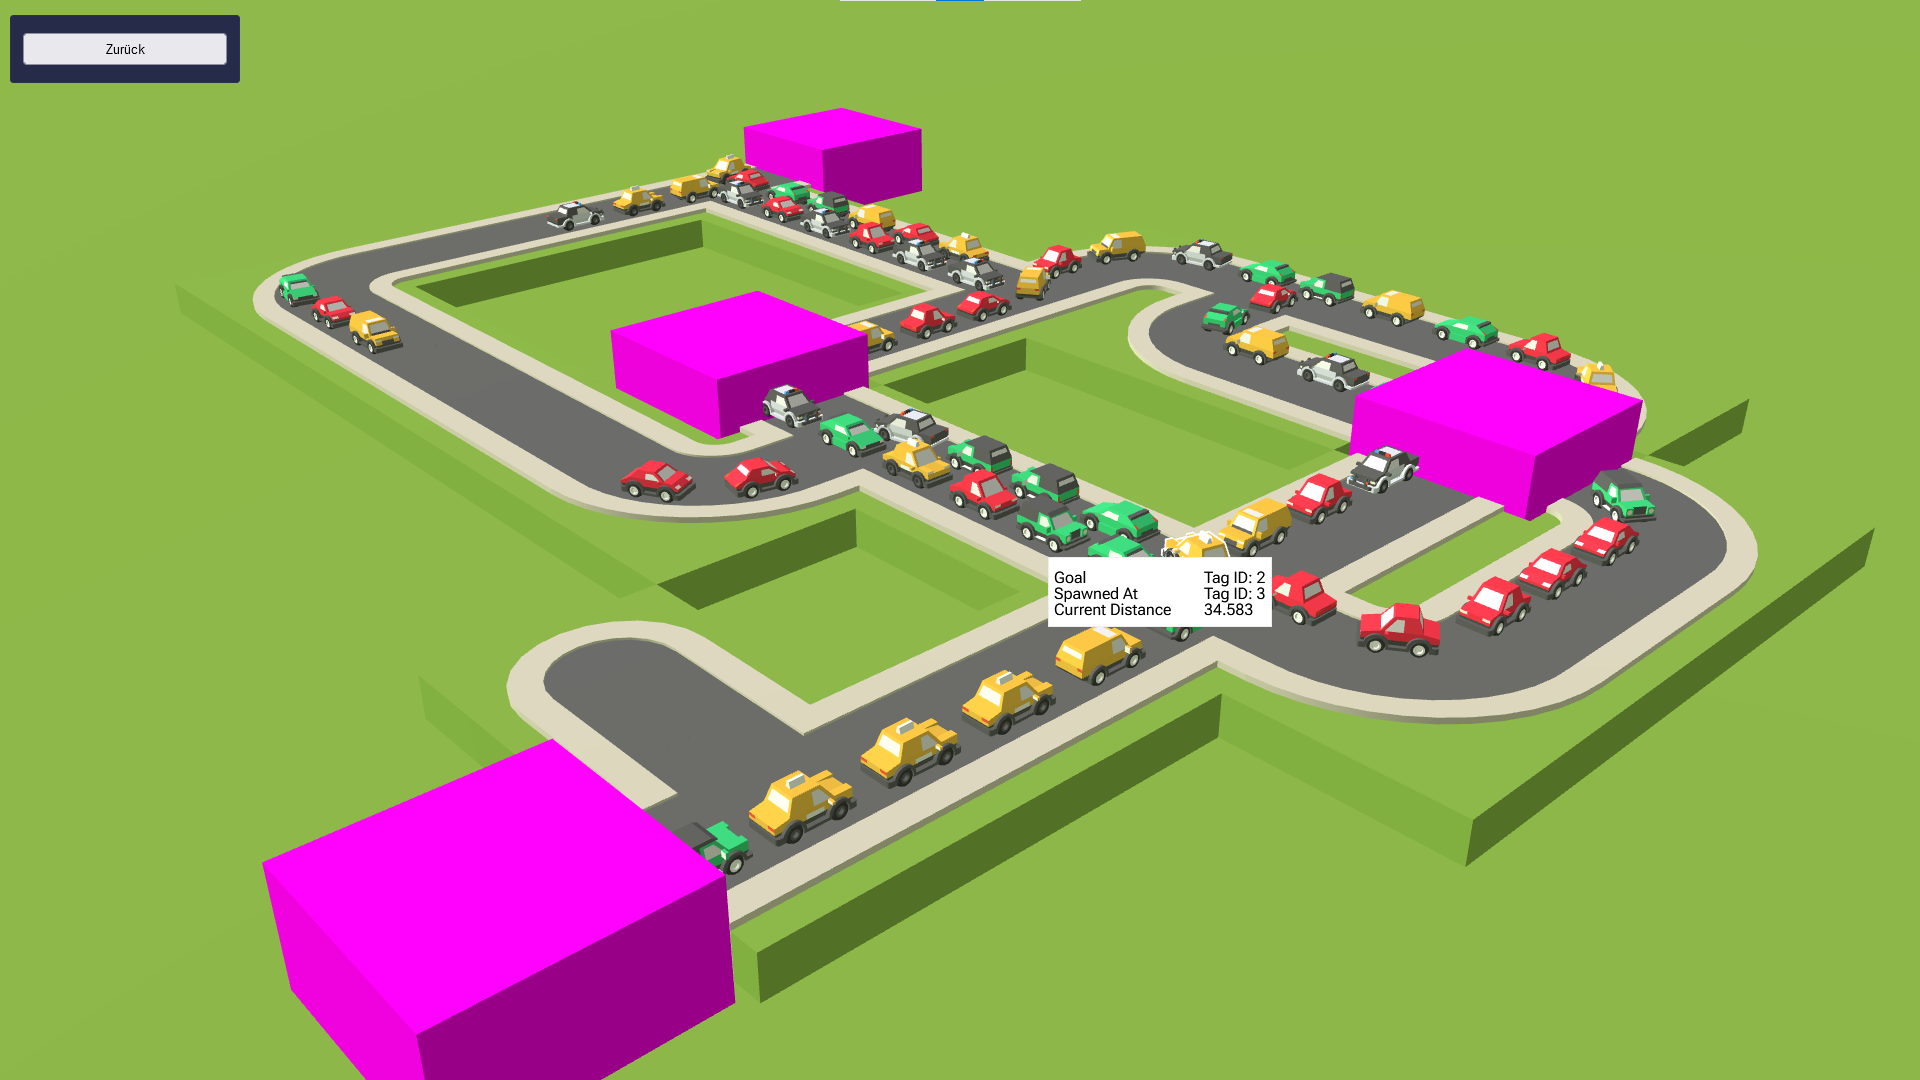
\includegraphics[scale=.25,center]{medien/screenshots/instance-view.png}
    \caption{Darstellung einer Instanz}
    \ownsource
    \label{fig:instance-view}
\end{figure}

Dies gelang vor allem deshalb, weil sich bei der Implementation von dem Node System\footnote{\url{https://docs.blender.org/manual/en/3.2/compositing/introduction.html}} \footnote{\url{
https://docs.blender.org/manual/en/3.2/render/shader_nodes/index.html}} der Blender Suite inspiriert worden lassen ist und dadurch die Implementation so abstrahiert werden konnte, dass sich die einzelnen Komponenten zielführend verbessern ließen.

Zusätzlich lassen sich durch die Export-Schnittstelle des Agenten auch Daten in Echtzeit an dem Fahrzeug anbringen und darstellen (siehe \refimg{fig:instance-view}), wodurch das Nachvollziehen des Verhaltens dieser Instanz noch einfacher wird.

Die gesamte Darstellung ist, wie gewünscht, in Echtzeit mit einer kontinuierlich guten Performance und einer hohen Bildwiederholrate möglich.

Insgesamt war die Implementation dieses Abschnitts die aufwendigste, insofern sie viele Komponenten umfasste und eine sehr solide Implementation voraussetzte.
Jedoch ist es gelungen, auch diese Anforderung wie gewünscht umzusetzen.


    \subsection{Quellcode und Artefakte} \label{sec:artefacts}

Die durch diese Entwicklung entstandenen Quelldateien, die Quelldateien für dieses Dokument, die Scripte zur Erschaffung der Artefakte sowie die vorgebauten Artefakte sind alle online frei zugänglich verfügbar.

Der gesamte Quellcode ist unter der GPL 3.0 Lizenz als Git-Repository auf GitHub verfügbar.
Dabei findet man in dem TRISS-Application Repository\footnote{\url{https://github.com/Feirell/triss-app-frozen}} die Quelldateien für alle Programm-Artefakte, unter dem TRISS-Documententation Repository\footnote{\url{https://github.com/Feirell/triss-doc-frozen}} sind die Quelldateien für dieses Dokument enthalten und im Dockerhub als \enquote{trissapp/triss-server}\footnote{\url{https://hub.docker.com/r/trissapp/triss-server}} das Backend bzw. als \enquote{trissapp/triss-client}\footnote{\url{https://hub.docker.com/r/trissapp/triss-client}} das Frontend.

Im TRISS-Application Repository\footnote{\url{https://github.com/Feirell/triss-app-frozen}} findet man neben dem Quellcode auch eine technische Einführung in das Projekt sowie eine kurze Anleitung für die Entwicklung eines Agenten.

In dieser technischen Einleitung findet man auch eine generelle Einführung in die Quellcode-Struktur und wie diese angepasst werden kann.
Zusätzlich ist dort auch beschrieben, wie sich die Artefakte in Betrieb nehmen lassen.

Darüber hinaus wurden im Kontext der Arbeit einige Artefakte erstellt, die einen generellen unabhängigen Mehrwert hatten und deshalb in das öffentliche npm-Repository ausgelagert worden sind.

Dazu zählen primär die folgenden drei Pakete.

Der \textit{performance-test-runner}\footnote{\url{https://npmjs.org/package/performance-test-runner}} ist ein Paket, das verwendet worden ist, um unterschiedliche Implementationen gegeneinander abzuwägen und somit stringent auf Verbesserungen hinzuarbeiten.

Bei dem Paket \textit{event-emitter-typesafe}\footnote{\url{https://npmjs.org/package/event-emitter-typesafe}} handelt es sich um eine Teil-Implementation des DOM-Standards für EventEmitter\autocite{domSpecEvent2022}, welche hier allerdings Typsicher implementiert worden ist und zusätzlich nicht die Runtime-Implementation benötigt und somit auch für Node.js Anwendung verwendet werden konnte.

Ebenso wurde das wichtige \textit{serialization-generator}\footnote{\url{https://npmjs.org/package/serialization-generator}} Paket ausgelagert.
Dieses ist, wie bereits zu erkennen war, von zentraler Bedeutung, da es die performante Übertragung der Simulationszustände zwischen den Realms erlaubt.
Hinzu kommt, dass darauf Wert gelegt worden ist, die Spezifikation der Datenstrukturen bzw. der (De-)Serialisierer sehr leserlich und intuitiv zu halten.




    \section{Ausblick}

Im Kontext dieser Projektarbeit sollte ein MVP erzeugt werden, der zum einen demonstriert, dass sich die Technologien des JavaScript Ökosystems dafür eignen, aber zum anderen auch, dass die gesamtheitliche Struktur und Architektur die gewünschten Funktionen bereitstellen können.

Jedoch gibt es Dinge, die noch im Rahmen dieses gemeinsamen Nenners liegen, sowohl funktional als auch in Hinblick auf die Verarbeitungseffizienz.

Diese zusätzlichen Punkte könnten im Kontext weiterer Entwicklungen in Betracht gezogen werden.



    \subsection{Funktionale Weiterentwicklungen}

\subsubsection{Generierung von Daten-Graphen}

Ein Beispiel für solch eine funktionale und universell praktische Funktion sind Daten-Graphen, die über den Verlauf der Simulation erzeugt werden und im Vorfeld programmatisch definiert worden sind.
Solch ein Graph könnte beispielweise die Anzahl der Fahrzeuge in jedem Frame darstellen oder die Zeit, die benötigt worden ist, um diesen zu erzeugen.
Dadurch ließe sich nicht nur ein Verlauf innerhalb einer konkreten Simulation erkennen, sondern auch eine Entwicklung im Hinblick auf unterschiedliche Versionen eines Agenten.

Diese Graphen würden dann mit der Instanz definiert werden und ließen sich dann im Anschluss via SVG/JSON exportiert.

\subsubsection{Speichern und Laden von Instanzen}

Ebenso praktisch wäre das Speichern und Laden von Instanzen, was so noch nicht mit eingebaut ist.
Die Herausforderung für das Speichern besteht darin, dass der Agent dann die Anforderung erfüllen muss seinen inneren Zustand exportieren können zu müssen.

Unabhängig davon wäre das praktisch für dies Testen von Langzeitverhalten und dafür, solche Instanzen dann von einem System in ein anderes transportieren zu können.

\subsubsection{Anpassen bzw. Färben von Modellen}

Eine weitere vorteilhafte Funktion wäre, wenn der Agent über die Weltdefinition die Fahrzeugmodelle einfärben könnte.
Das würde dem Agenten erlauben dadurch gewisse Eigenschaften des Fahrzeuges sehr einfach und offensichtlich zu repräsentieren.

Beispielweise könnte der Agent das nutzen, um Fahrzeuge je nach dem Fahrerprofil einzufärben, beispielweise könnte Rot dann einen \enquote{Drängler} und Blau einen \enquote{Sonntagsfahrer} darstellen.

\subsubsection{Konfigurierbare Straßen, Fahrspuren und Kreuzungen}

Frei konfigurierbare Straßen würde der Simulation bedeutende Modellfeinheit geben, vor allem im Hinblick auf die Situationen, in denen man den Agenten testen könnte.

So ist es aktuell nicht ohne Weiteres möglich, Überholvorgänge durch eine parallele Fahrbahn durchzuführen, da keine Kachel existiert, die solch eine Fahrbahn vordefiniert bereitstellen würde.
Zusätzlich wäre die Möglichkeit, Straßen nicht nur nach einem Kachelmuster setzten zu können, vorteilhaft, um andere Konstellationen für den Agenten zu schaffen.

Hinzu kommt, dass durch ein feiner definierbares Straßennetz auch die Möglichkeit entsteht, mit einem entsprechend komplexen Agenten Rückschlüsse auf den realen Straßenverkehr zu ziehen.

\subsubsection{Local Computation} \label{sec:fnc-impr-local-computation}

Ein großer praktischer Nutzen würde dadurch entstehen, wenn man bei dem Anlegen einer Instanz definieren könnte, wo diese betrieben werden soll.
So könnte man definieren, dass diese direkt im Browser in einem eigenen Worker die Frames errechnet.

Dies würde die Latenz drastisch verringern und erlauben, diese Anwendung ausschließlich mit einem statischen HTTP-Server und einem Webbrowser zu betreiben.
Dieser letzte Punkt ist insofern besonders hilfreich, als eine zentrale Instanz, wie beispielweise GitHub Pages, die Assets und Bundles bereitstellt und der Nutzer die eigentliche Rechenleistung für die Berechnung der Frames und die Darstellung dieser.

Somit könnte man diese kostengünstig darüber anbieten, ohne die eigentliche Rechenleistung mit in Betracht ziehen zu müssen, und der Nutzer kann ohne Installation oder Server die Anwendung ausprobieren und verwenden.


    \subsection{Verarbeitungsgeschwindigkeits-Verbesserungen}

Zusätzlich zu den beschriebenen funktionalen Verbesserungen bestehen auch Möglichkeiten die Performance der Anwendung weiter zu verbessern.

Einen kleinen Ausschnitt möglicher Weiterentwicklungen soll im Folgenden gegeben werden.

\subsubsection{Frame Caching}

Wie in der \refsec{sec:reflection-main} angedeutet, ist ein größeres Problem die Übertragungslatenzen, die die Bildwiederholrate negativ beeinflussen kann.
Diesem könnte entgegengewirkt werden, indem die Zwischenstationen, also der Simulation Instance Realtime Handler, der Individual WebSocket Handler und der Server Connector, mehrere Frames vorhalten und diese dadurch regelmäßiger übertragen bzw. bereitstellen könnten.

Die Herausforderung dabei ist jedoch, dass dieses Zwischenspeichern in Balance mit dem Speichervolumen und der Verzögerung durch diese gehalten werden muss.
Zusätzlich erhöht sich die Komplexität durch die unterschiedlichen Verarbeitungsgeschwindigkeiten der beteiligten Rechensysteme.

Wenn zum Beispiel Client A die Zustände mit 30 Hz darstellen kann, Client B mit 60 Hz und der Agent sie mit 45 Hz produziert, dann ist es hier nicht trivial, diese Caches zu implementieren, sodass sie tatsächlich unterstützen und nicht die Darstellung behindern.

Hinzu kommt, dass dann die neu angefragte Exported Agent Data nicht mehr direkt im nächsten Frame bereitgestellt werden könnte, sondern einige Frames Latenz hätten, insofern die neuen Informationen erst einmal durch alle Caches traversieren müsste.

\subsubsection{(De-)Serialisierung implizieren}

Ein großer Vorteil würde sich dadurch ergeben, wenn die (De-)Serialisierung nicht mehr explizit in einem Schritt durchgeführt werden würde, sondern das System und die Agenten direkt auf der Binärrepräsentation arbeiten würden und dadurch keine volle (De-)Serialisierung mehr benötigt wird.

Dies hätte allerdings einen enormen Änderungsaufwand für diese Anwendung bedeutet, deshalb wurde dies hier nicht mehr in Betracht gezogen.

Zentral wäre dabei, die 25 \% der Zeit im Client für die Garbage Collection zu reduzieren und den diskreten Schritt der Deserialisierung und Objekterstellung auszusparen.

Gerade letztere überwiegt den eigentlichen Darstellungsaufwand bei Weitem und würde somit viel Zeit für die Darstellung bzw. die Erzeugung freimachen.

Idealerweise würde der übertragene Frame vom Agenten direkt in den GPU Buffer geschrieben werden und dann durch einen entsprechenden Shader in die notwendige Darstellung umgeformt werden.

\subsubsection{Frame Skipping}

Wie sich im Kapitel \refsec{sec:reflection-main} erkennen ließ, ist die Serialisierung ein beschränkender Faktor.
Die bereits beschriebenen Überlegungen könnten diesen drastisch verringern, jedoch sind sie alle sehr aufwendig in der Implementation.

Einfacher wäre es da das System so zu erweitern, dass die Darstellung, Erzeugung und (De-)Serialiserung im Gleichgewicht gehalten wird, in dem Frames zwar errechnet werden, jedoch nicht Serialisiert und Übertragen werden.

Diese Anpassung ist aber ähnlich wie das Caching nicht vollständig trivial, wenn mehrere Consumer und Fluktuationen in der Latenz und Übertragungsgeschwindigkeit mit in Betracht gezogen werden.
Sie besitz allerdings ein bedeutend besseres Aufwand/Resultat Verhältnis als es beispielweise das Implizieren oder Cachen hat.



    \newpage

\section{Fazit}

Insgesamt ist dieses Projekt ein Erfolg.
Es ist gelungen, eine Test-Implementation einer Simulations-Plattform für die Echtzeitdarstellung von Simulationszuständen eines Agenten im Kontext der Verkehrsdomäne zu erschaffen.

Abschließend lässt sich sagen, dass die initiale Fragestellung, ob sich solch eine Agenten-Simulationsplattform mit dem JavaScript Ökosystem realisieren lässt, mit \enquote{Ja} beantwortet werden kann.

Die angestrebte Plattform ließ sich nicht nur im Hinblick auf die nicht funktionalen Anforderungen mit diesen Technologien realisieren, sondern konnte darüber hinaus auch die angestrebte hohe Performance erreichen, die selbst die Implementation und Auswertung von mittelgroßen Agenten mithilfe einer Echtzeit-3D-Darstellung erlaubt.

Es muss allerdings auch festgehalten werden, dass es noch viele Wege gäbe, die Anwendung zu erweitern und zu verbessern.
Vor allem durch den Punkt \refsec{sec:fnc-impr-local-computation} ließe sich die Verwendung bedeutend weiter vereinfachen, sodass noch mehr Menschen von ihr profitieren könnten.

Insgesamt ließ sich jedoch eine sehr solide Plattform erschaffen, die bereits jetzt einen relevanten Mehrwert bietet und auch ohne weitere Anpassungen für unterschiedliche Anwender und andere interessierte Entwickler als Beispiel-Implementation nützlich sein kann.



    \newpage

%    \section{Abbildungsverzeichnis}

    \listoffigures


%    \section{Tabellenverzeichnis}

    \listoftables


%    \section{Literaturverzeichnis}

    \printbibliography[title=Literaturverzeichnis]

\end{document}
